\documentclass[12pt,spanish,Letterpaper,openany]{book}
\usepackage{lmodern}
\usepackage{setspace}
\setstretch{1.0}
\usepackage{amssymb,amsmath}
\usepackage{ifxetex,ifluatex}
\usepackage{fixltx2e} % provides \textsubscript
\ifnum 0\ifxetex 1\fi\ifluatex 1\fi=0 % if pdftex
  \usepackage[T1]{fontenc}
  \usepackage[utf8]{inputenc}
\else % if luatex or xelatex
  \ifxetex
    \usepackage{mathspec}
  \else
    \usepackage{fontspec}
  \fi
  \defaultfontfeatures{Ligatures=TeX,Scale=MatchLowercase}
    \setmainfont[Scale=0.93, HyphenChar=None]{Open Sans}
    \setsansfont[]{Open Sans}
    \setmonofont[Mapping=tex-ansi]{Open Sans}
\fi
% use upquote if available, for straight quotes in verbatim environments
\IfFileExists{upquote.sty}{\usepackage{upquote}}{}
% use microtype if available
\IfFileExists{microtype.sty}{%
\usepackage{microtype}
\UseMicrotypeSet[protrusion]{basicmath} % disable protrusion for tt fonts
}{}
\usepackage[left=10mm,right=10mm,top=11mm,bottom=20mm]{geometry}
\usepackage{hyperref}
\hypersetup{unicode=true,
            pdftitle={Decimocuarta Edición - ECYS},
            pdfauthor={Escuela de Ingeniería en Ciencias y Sistemas.},
            pdfborder={0 0 0},
            breaklinks=true}
\urlstyle{same}  % don't use monospace font for urls
\ifnum 0\ifxetex 1\fi\ifluatex 1\fi=0 % if pdftex
  \usepackage[shorthands=off,main=spanish]{babel}
\else
  \usepackage{polyglossia}
  \setmainlanguage[]{spanish}
\fi
\usepackage{natbib}
\bibliographystyle{apalike}
\usepackage{longtable,booktabs}
\usepackage{graphicx,grffile}
\makeatletter
\def\maxwidth{\ifdim\Gin@nat@width>\linewidth\linewidth\else\Gin@nat@width\fi}
\def\maxheight{\ifdim\Gin@nat@height>\textheight\textheight\else\Gin@nat@height\fi}
\makeatother
% Scale images if necessary, so that they will not overflow the page
% margins by default, and it is still possible to overwrite the defaults
% using explicit options in \includegraphics[width, height, ...]{}
\setkeys{Gin}{width=\maxwidth,height=\maxheight,keepaspectratio}
\IfFileExists{parskip.sty}{%
\usepackage{parskip}
}{% else
\setlength{\parindent}{0pt}
\setlength{\parskip}{6pt plus 2pt minus 1pt}
}
\setlength{\emergencystretch}{3em}  % prevent overfull lines
\providecommand{\tightlist}{%
  \setlength{\itemsep}{0pt}\setlength{\parskip}{0pt}}
\setcounter{secnumdepth}{5}

%%% Use protect on footnotes to avoid problems with footnotes in titles
\let\rmarkdownfootnote\footnote%
\def\footnote{\protect\rmarkdownfootnote}


  \title{Decimocuarta Edición - ECYS}
    \author{Escuela de Ingeniería en Ciencias y Sistemas.}
      \date{2019-08-01}

%%%%%%%%%%%%%%%%%%%%%%%%%%%%%%%%%%%%%%%%%%%%%%%INIT PREAMBLE%%%%%%%%%%%%%%%%%%%%%%%%%%%%%%%%%%%%%%%%%%%%%%%


%% Opcion que renueva los comandos para el cambio de seccion, el comando por defecto para cada cambio de
%%% seccion genera una pagina en limpio, por lo tanto se renueva el comando definiendo que no se
%%% realice ese cambio, dado que no es funcionan para la edicion de la revista.
%%% Se define para la seccion frontmatter (portada, editorial y contenido) la numeracion de la pagina 
%%% en formato arabico, para la mainmatter (seccion principal - capitulos) la numeracion en numeracion romana (numeros
%%% enteros), y para seccion backmatter ningun tipo de numeracion.
\makeatletter
\renewcommand\mainmatter{\clearpage\@mainmattertrue\pagenumbering{arabic}}
\renewcommand\frontmatter{\clearpage\@mainmatterfalse\pagenumbering{roman}}
\renewcommand\backmatter{\clearpage\@mainmatterfalse}
\makeatother



%% Paquete para el manejo de titulos de capitulos y secciones
\usepackage[explicit,pagestyles]{titlesec}
%% Paquete para uso de urls
\usepackage{url}
%% Paquete utilizado para establecer doble columna en la redaccion de articulos
\usepackage{multicol}
%% Paquete para parametro H, ejemplo: \begin{Figure}[H]
\usepackage{float}
%% Paquete para Enmarcado de Biografia Estudiante, ejemplo: \begin{tcolorbox}...
\usepackage{tcolorbox}
%% Paquete para cargar portada y contraportada, ejemplo: 
\includepdf{01-componentsPDF/cover.pdf}
%% Manual: http://mirrors.ucr.ac.cr/CTAN/macros/latex/contrib/pdfpages/pdfpages.pdf
\usepackage{pdfpages}
%% Paquete para cargar paginas de disenio, ejemplo: \AddEverypageHook{%
\usepackage[contents={},opacity=1,scale=1.5,color=blue!90]{background}
%% Paquete para usar instruccion \ifthenelse
\usepackage{ifthen}
%% Paquete para la definicion de footers y headers
\usepackage{fancyhdr}
%% Paquete complemento para definir tamanio de texto al setear footer y headers
\usepackage{varwidth}
%% Paquete para uso de region sombreada utilizada en titulos de la revista
\usepackage{framed}
%% Paquete utilizado para redefinir tabulacion de vinietas
\usepackage{enumitem}

%% Opcion que define el cambio de linea colocando '-', a las urls demasiado grandes
\def\UrlBreaks{\do\/\do-}

%% Definicion de Comando que acepta un valor numerico y agrega un cero a la izquierda
%%% en el caso que el numero sea menor a 10, se ocupa para la numeracion de las 
%%% paginas iniciales
\newcommand\twodigits[1]{%
   \ifnum#1<10 0#1\else #1\fi
}

%% Instruccion que define a las imagenes la posibilidad de tener un link (interno o
%%% externo activo; se utiliza para enlazar las imagenes a los capitulos definidos
%%% en la hoja del contenido
\ifxetex
  \usepackage{letltxmacro}
  \setlength{\XeTeXLinkMargin}{1pt}
  \LetLtxMacro\SavedIncludeGraphics\includegraphics
  \def\includegraphics#1#{% #1 catches optional stuff (star/opt. arg.)
    \IncludeGraphicsAux{#1}%
  }%
  \newcommand*{\IncludeGraphicsAux}[2]{%
    \XeTeXLinkBox{%
      \SavedIncludeGraphics#1{#2}%
    }%
  }%
\fi

%%%%%%%%%%%%%%%%%%%%%%%INIT Definicion de Numeracion de Paginas%%%%%%%%%%%%%%%%%%%%

%% Seteo de Numero de Pagina, con 2 digitos (01-99) y numeros en negritas %
\newcommand{\etiquetaNumberPage}{%
  %% Manual comando \fontspec: http://mirrors.ucr.ac.cr/CTAN/macros/latex/contrib/fontspec/fontspec.pdf %
  %% \fontspec{(font name)}[(font features)] %
  %%% Es uno de los comandos ad hoc más adecuados para probar y cargar fuentes de forma única. %
  \fontspec{%
    %% Nombre de Fuente Instalada en la carpeta Fonts de Windows "C:\Windows\Fonts" %
    Helvetica Neue LT W1G%
  }[%
    %% SizeFeatures={Size=(X)} %%
    %%% opcion que define diferentes caracteristias para diferentes tamanios de fuente; %
    %%% se utiliza un tamanio (x=numero) con la caracteristica "Size". %
    %
    %% Tamanio de Fuente: 17 %
            SizeFeatures={Size=32},%
    %% Color=(color) %
    %%% Utiliza especificaciones del font para establecer el color del texto.
    %
    %% Color del Texto: Blanco
            Color=white,%
    %% WordSpace={x} %
    %%% toma un factor de escala para escalar el valor predeterminado de espacio entre palabras
    %
    %% Valor para espacio entre palabras: 0 - estrecho %
            %WordSpace=0.0,%
    %% LetterSpace={x}%
    %%% termino dado a sumar (o restar) una pequenia cantidad de espacio horizontal entre caracteres %
    %%% adyacentes; toma un argumento numérico; es un factor aditivo normalizado (no un factor de % 
    %%% escala); Se define como un porcentaje del tamaño de fuente. %
    %
    %% valor de espaciado entre letras: -11.8 - muy estrecho%
            %LetterSpace=-2.5%
  ]%
  %% Commando \twodigits{numero} %
  %%%  devuelve numero en formato de 2 digitos (01-99) %
  \twodigits{%
    %% comando \thepage %
    %%% indica el numero de pagina %
    \thepage%
  }%
}
%%%%%%%%%%%%%%%%%%%%%%%END Definicion de Numeracion de Paginas%%%%%%%%%%%%%%%%%%%%%%%

%%%%%%%%%%%%%%%%%%%%%%%INIT Definicion de Etiquetas de Revista%%%%%%%%%%%%%%%%%%%%%%%

%% Seteo Etiqueta Ciencias, Sistemas y Tecnologia, vinculada con el enlace
%% de la Escuela de Ingenieria en Ciencias y Sistemas
\newcommand{\etiquetaCienciasSistemasTecnologia}{%
  %% Manual comando \fontspec: http://mirrors.ucr.ac.cr/CTAN/macros/latex/contrib/fontspec/fontspec.pdf %
  %% \fontspec{(font name)}[(font features)] %
  %%% Es uno de los comandos ad hoc más adecuados para probar y cargar fuentes de forma única. %
  \fontspec{%
    %% Nombre de Fuente Instalada en la carpeta Fonts de Windows "C:\Windows\Fonts" %
    OCR A Extended%
  }[%
    %% SizeFeatures={Size=(X)} %%
    %%% opcion que define diferentes caracteristias para diferentes tamanios de fuente; %
    %%% se utiliza un tamanio (x=numero) con la caracteristica "Size". %
    %
    %% Tamanio de Fuente: 12 %
            SizeFeatures={Size=12},%
    %% Color=(color) %
    %%% Utiliza especificaciones del font para establecer el color del texto.
    %
    %% Color del Texto: Blanco
            Color=white,%
    %% WordSpace={x} %
    %%% toma un factor de escala para escalar el valor predeterminado de espacio entre palabras
    %
    %% Valor para espacio entre palabras: 0 - estrecho %
            %WordSpace=0.8,%
    %% LetterSpace={x}%
    %%% termino dado a sumar (o restar) una pequenia cantidad de espacio horizontal entre caracteres %
    %%% adyacentes; toma un argumento numérico; es un factor aditivo normalizado (no un factor de % 
    %%% escala); Se define como un porcentaje del tamaño de fuente. %
    %
    %% valor de espaciado entre letras: -4.5 - estrecho%
            LetterSpace=-4.5%
  ]%
  %% \href{(url)}{(description)} %
  \href{}{}%
}

%% Seteo Etiqueta Facultad de Ingenieria, vinculada con el enlace
%% de la pagina de ingenieria
\newcommand{\etiquetaFacultadDeIngenieria}{%
  %% Manual comando \fontspec: http://mirrors.ucr.ac.cr/CTAN/macros/latex/contrib/fontspec/fontspec.pdf %
  %% \fontspec{(font name)}[(font features)] %
  %%% Es uno de los comandos ad hoc más adecuados para probar y cargar fuentes de forma única. %
  \fontspec{%
    %% Nombre de Fuente Instalada en la carpeta Fonts de Windows "C:\Windows\Fonts" %
    OCR A Extended%
  }[%
    %% SizeFeatures={Size=(X)} %%
    %%% opcion que define diferentes caracteristias para diferentes tamanios de fuente; %
    %%% se utiliza un tamanio (x=numero) con la caracteristica "Size". %
    %
    %% Tamanio de Fuente: 17 %
            SizeFeatures={Size=12},%
    %% Color=(color) %
    %%% Utiliza especificaciones del font para establecer el color del texto.
    %
    %% Color del Texto: Blanco
            Color=white,%
    %% WordSpace={x} %
    %%% toma un factor de escala para escalar el valor predeterminado de espacio entre palabras
    %
    %% Valor para espacio entre palabras: 0 - estrecho %
            %WordSpace=0.0,%
    %% LetterSpace={x}%
    %%% termino dado a sumar (o restar) una pequenia cantidad de espacio horizontal entre caracteres %
    %%% adyacentes; toma un argumento numérico; es un factor aditivo normalizado (no un factor de % 
    %%% escala); Se define como un porcentaje del tamaño de fuente. %
    %
    %% valor de espaciado entre letras: -11.8 - muy estrecho%
            LetterSpace=-4.5%
  ]%
  %% \href{(url)}{(description)} %
  \href{}{}%
}
%%%%%%%%%%%%%%%%%%%%%%%END Definicion de Etiquetas de Revista%%%%%%%%%%%%%%%%%%%%%%%

%%%%%%%%%%%%%%%%%INIT Aplicando Estilos de Numeros de Pagina y Etiquetas de Revista%%%%%%%%%%%%%%%%%


%% Seteo de Numero de Pagina en la parte derecha, para paginas pares (Even)
\newcommand{\nodeNumberPageEast}{%
  %% Manual comando \node: http://mirrors.ucr.ac.cr/CTAN/graphics/pgf/base/doc/pgfmanual.pdf %
  \node[%
    %% /tikz/anchor=(anchor) %
    %%% Specifies an anchor of the node; %
    %
    %% anclaje abajo izquierda %
        anchor=south west,% 
    %% /tikz/text=(color) %
    %%% Sets the color to be used for text labels; %
    %
    %% color de texto blanco %
        text=black,%
    %% /tikz/execute at begin node=(code) %
    %%% Esta opcion hace que (code) se ejecute al principio de un nodo
        execute at begin node={\begin{varwidth}{\textheight}}, %
    %% /tikz/execute at end node=(code) %
    %%% Esta opcion instala (code) que se ejecutará al final del nodo
        execute at end node={\end{varwidth}}%
  ]%
  %
  %% Current Page Node – Absolute Positioning %
  %% There is a special node called current page that can be used to access the current page. %
  %
  %% ubicacion de pagina abajo derecha %
  at ([xshift=-21mm,yshift=1.7mm] current page.south east)% 
  {\etiquetaNumberPage};%
}

%% Seteo de Numero de Pagina en la parte izquierda, para paginas impares (Odd)
\newcommand{\nodeNumberPageWest}{%
  %% Manual comando \node: http://mirrors.ucr.ac.cr/CTAN/graphics/pgf/base/doc/pgfmanual.pdf %
  \node[%
    %% /tikz/anchor=(anchor) %
    %%% Specifies an anchor of the node; %
    %
    %% anclaje abajo izquierda %
        anchor=south west,% 
    %% /tikz/text=(color) %
    %%% Sets the color to be used for text labels; %
    %
    %% color de texto blanco %
        text=black,%
    %% /tikz/execute at begin node=(code) %
    %%% Esta opcion hace que (code) se ejecute al principio de un nodo
        execute at begin node={\begin{varwidth}{\textheight}}, %
    %% /tikz/execute at end node=(code) %
    %%% Esta opcion instala (code) que se ejecutará al final del nodo
        execute at end node={\end{varwidth}}%
  ]%
  %
  %% Current Page Node – Absolute Positioning %
  %% There is a special node called current page that can be used to access the current page. %
  %
  %% ubicacion de pagina abajo izquierda %
  at ([xshift=9mm,yshift=1.7mm] current page.south west)%
  {\etiquetaNumberPage};%
}

%% Comando que establece la posicion horizontal de la Etiqueta Ciencias, Sistemas y Tecnologia %
%% Por medio del comando \node%
\newcommand{\nodeHorizontalPositionCienciasSistemasTecnologia}{%
  %% Manual comando \node: http://mirrors.ucr.ac.cr/CTAN/graphics/pgf/base/doc/pgfmanual.pdf %
  \node[%
    %% /tikz/text=(color) %
    %%% Sets the color to be used for text labels; %
    %
    %% color de texto white %
    text=white, %
    %% /tikz/execute at begin node=(code) %
    %%% Esta opcion hace que (code) se ejecute al principio de un nodo
    execute at begin node={\begin{varwidth}{\textheight}}, %
    %% /tikz/execute at end node=(code) %
    %%% Esta opcion instala (code) que se ejecutará al final del nodo
    execute at end node={\end{varwidth}}%
  ]%
  %
  %% Current Page Node – Absolute Positioning %
  %% There is a special node called current page that can be used to access the current page. %
  %
  %% ubicacion de pagina abajo derecha %
  at ([xshift=-67.50mm,yshift=5mm]current page.south east)%
  {\etiquetaCienciasSistemasTecnologia};%
}
%% Comando que establece la posicion horizontal de la Etiqueta Facultad de Ingenieria %
%% Por medio del comando \node%
\newcommand{\nodeHorizontalPositionFacultadDeIngenieria}{%
  %% Manual comando \node: http://mirrors.ucr.ac.cr/CTAN/graphics/pgf/base/doc/pgfmanual.pdf %
  \node[%
    %% /tikz/text=(color) %
    %%% Sets the color to be used for text labels; %
    %
    %% color de texto white %
    text=white, %
    %% /tikz/execute at begin node=(code) %
    %%% Esta opcion hace que (code) se ejecute al principio de un nodo
    execute at begin node={\begin{varwidth}{\textheight}}, %
    %% /tikz/execute at end node=(code) %
    %%% Esta opcion instala (code) que se ejecutará al final del nodo
    execute at end node={\end{varwidth}}%
  ]%
  %
  %% Current Page Node – Absolute Positioning %
  %% There is a special node called current page that can be used to access the current page. %
  %
  %% ubicacion de pagina abajo izquierda %
  at ([xshift=66.5mm,yshift=5mm]current page.south west)
  {\etiquetaFacultadDeIngenieria};%
}

%% Aplicando segundo estilo de numeracion y etiquetas
%%% Numeracion parte inferior derecha e izquierda 
%%%% numeros impares = izquierda: Footer Odd
%%%% numeros pares = derecha: Footer Even
%%%
%%% Etiquetas parte derecha e izquierda
%%%% etiqueta Facultad de Ing. = izquierda: Footer Odd
%%%% etiqueta Ciencias Sistemas. = Derecha: Footer Even
%%%
%% Comando con nombre "fancyplainstyle", que identifica el
%%% primer estilo a representar en la revista.
\newcommand{\fancyplainstyleTwo}{
  %% Comando que limpia cualquier personalizacion antes realizada
  %%% para el borrado completo no agregar ningun parametro "{}"
  \fancyhf{}
  %% Definiendo etiqueta horizontal Ciencias Sistemas
  %% Definiendo numero de pagina par
  %%% \fancyfoot[places]{field}
  \fancyfoot[E]{
    %% Comando que se define para establecer posicion absoluta de
    %%% etiqueda de acuerdo a las posiciones defindas en la declaracion
    %%% del comando \nodeHorizontalPosition...
    \begin{tikzpicture}[overlay, remember picture]%
      \nodeNumberPageEast
      \nodeHorizontalPositionCienciasSistemasTecnologia
    \end{tikzpicture}
  }
  %% Definiendo etiqueta horizontal Facultad de Ing.
  %% Definiendo numero de pagina impar
  %%% \fancyfoot[places]{field}
  \fancyfoot[O]{
    %% Comando que se define para establecer posicion absoluta de
    %%% etiqueda de acuerdo a las posiciones defindas en la declaracion
    %%% del comando \nodeHorizontalPosition...
    \begin{tikzpicture}[overlay, remember picture]%
      \nodeNumberPageWest
      \nodeHorizontalPositionFacultadDeIngenieria
    \end{tikzpicture}
  }
}

%% Declarando comando que establece el primer tipo de estilo a todas las paginas,
%%% asi como tambien a las paginas donde se define el titulo del articulo,
%%% dado que el disenio es diferente al resto de las paginas.
\newcommand{\setPageStyleTwo}{%
  %% Definiendo el estilo a todas las paginas
  \pagestyle{fancy}{\fancyplainstyleTwo}
  %% Definiendo el mismo estilo a paginas que tiene el encabezado de titulo
  \fancypagestyle{plain}{\fancyplainstyleTwo}
}

%% Borrando estilos de paginas que forman parte del frontmatter (editorial y
%%% contenido), dado que dichas paginas tienen una estructura unica
\fancypagestyle{plain}{%
  %% Comando que limpia cualquier personalizacion antes realizada
  %%% para el borrado completo no agregar ningun parametro "{}"
  \fancyhf{}%
}

%% Estableciendo tamanio de encabezado debido a warning mostrado al generar
%%% documento PDF, se establecio la longiutd de 15pt, por solicitud en contenido
%%% del mensaje mostrado en dicho warning.
\setlength{\headheight}{15pt}

%% El segmento de encabezado y pie de pagina, por default cuentan con una linea
%%% que divide los segmentos con el contenido del documento, por disenio de revista
%%% las lineas no son requeridas, por lo tanto se define el grosor de la linea con
%%% valor 0 (cero).
\renewcommand{\headrulewidth}{0pt}
\renewcommand{\footrulewidth}{0pt}

%%%%%%%%%%%%%%%%%%END Aplicando Estilos de Numeros de Pagina y Etiquetas de Revista%%%%%%%%%%%%%%%%%

%%%%%%%%%%%%%%INIT Definicion Region sombreada para titulo y datos de author de articulo%%%%%%%%%%%%%%
\definecolor{fondo}{HTML}{BFBFBF}
\definecolor{fondotitulo}{HTML}{0870B7}
\colorlet{shadecolor}{fondotitulo}
%%%%%%%%%%%%%%END Definicion Region sombreada para titulo y datos de author de articulo%%%%%%%%%%%%%%

%%%%%%%%%%%%%%INIT Dehabilitando Titulo y Autor por Default%%%%%%%%%%%%%%
\AtBeginDocument{\let\maketitle\relax}
%%%%%%%%%%%%%%END Dehabilitando Titulo y Autor por Default%%%%%%%%%%%%%%

%%%%%%%%%%%%%%INIT Propiedades de Parrafos, tabulaciones, vinietas, etc.%%%%%%%%%%%%%%

%% Cambiando longitud (setlength) de sangria de parrafos (\parindent)
%%% 1em es equivalente al espacio de una 'M' de acuerdo al tipo y tamanio de fuente.
\setlength{\parindent}{1em}
%% Cambiando longitud (setlist) de venietas (itemsize)
%%% 1em es equivalente al espacio de una 'M' de acuerdo al tipo y tamanio de fuente.
\setlist[itemize]{labelindent = \parindent, leftmargin=*}

%% Redefiniendo longitud minima de fraccion de texto ocupado en una pagina de texto
%%% valor por defecto 0.2
\renewcommand{\textfraction}{0.05}
%% Redefiniendo longitud maxima de fraccion de una pagina de texto ocupada por objetos
%%% flotantes en la parte superior, valor por defecto 0.7
\renewcommand{\topfraction}{0.8}
%% Redefiniendo longitud maxima de fraccion de una pagina de texto ocupada por objetos
%%% flotantes en la parte inferior, valor por defecto 0.3
\renewcommand{\bottomfraction}{0.8}
%% Redefiniendo longitud minima de fraccion de una pagina de texto ocupada por objetos
%%% flotantes que puede ser usada por los mismo, valor por defecto 0.5
\renewcommand{\floatpagefraction}{0.75}

%% Comando que establece el uso de espacio normal despues del signo '.'
\frenchspacing
%% La configuracion influye en la rutina de salto de parrafo en si misma: los cambios en 
%% \tolerance en realidad afectan a que saltos de linea se eligen. Los valores mas altos 
%% permiten que se acepten lineas peores (lo que generalmente significa: con espacios entre 
%% palabras estirados), con el valor que 10000indica un "modo de panico" donde cualquier cosa 
%% es aceptable. Normalmente, cuanto mas bajo sea el valor, mejor se vera el parrafo, pero corre 
%% el riesgo de reducir tanto la lista de posibles saltos que terminara con lineas demasiado llenas.
\tolerance=5000
%% quita la restriccion para igualar el contenido de la pagina (justificacion vertical)
\raggedbottom
%%%%%%%%%%%%%%END Propiedades de Parrafos, tabulaciones, vinietas, etc.%%%%%%%%%%%%%%

%%%%%%%%%%%%%%INIT Propiedades MultiColumnas%%%%%%%%%%%%%%
%% que contiene el valor de \pretolerance dentro de un entorno multicols 
\multicoltolerance=3000 
%% quita la restriccion para igualar el contenido en columnas (justificacion vertical)
\raggedcolumns
%% Espacio entre columnas esta controlado por el parámetro \setlength{\columnsep}
\setlength{\columnsep}{2em}
%We want a rule between columns.
%\setlength\columnseprule{.4pt}

%Tambien queremos asegurarnos de que un nuevo entorno multicols 
%encuentre suficiente espacio en la parte inferior de la página.
\setlength\premulticols{6\baselineskip}

%Al equilibrar columnas, ignoramos las soluciones que son 
%demasiado malas. Además, si la última columna es demasiado mala, 
%la tipeamos sin estirar.
\setcounter{columnbadness}{7000}
\setcounter{finalcolumnbadness}{7000}
%%%%%%%%%%%%%%END Propiedades MultiColumnas%%%%%%%%%%%%%%

\newenvironment{photobiography3}[1]%
{%
\begin{tcolorbox}[colback=fondo, colframe=fondo, width=95.19mm, boxsep=-2mm, arc=0mm]
\begin{minipage}{93.19mm}%
	\hspace{1mm}%
	\begin{minipage}{22.49mm}
	  \vspace{1mm}%
		\includegraphics[width=22.49mm, height=31.96mm]{#1}%
		\vspace{1mm}%
	\end{minipage}%
	\hspace{2.4mm}%
	\begin{minipage}{66.80mm}\begin{flushleft}\small%
}%
{%
	\end{flushleft}\end{minipage}%
	%\hspace{0.5mm}%
\end{minipage}%
\end{tcolorbox}
}

\newenvironment{photobiography4}%
{%
\begin{tcolorbox}[colback=fondo, colframe=fondo, width=92.19mm, boxsep=-2mm, arc=0mm]
\begin{minipage}{90.19mm}%
	\hspace{1mm}%
	\hspace{2.19mm}%
	\begin{minipage}{89.00mm}\begin{flushleft}\small%
	\vspace{3mm}%
}%
{%
  \vspace{3mm}%
	\end{flushleft}\end{minipage}%
	%\hspace{0.5mm}%
\end{minipage}%
\end{tcolorbox}
}




\newenvironment{boldenv}
  {\bfseries}% \begin{boldenv}
  {}% \end{boldenv}
  
\newenvironment{normalsizeenv}
  {\normalsize}% \begin{normalsizeenv}
  {}% \end{normalsizeenv}
  
\newenvironment{smalltextenv}
  {\begin{center}\kern-1em\color{fondotitulo}\small}% \begin{smalltextenv}
  {\end{center}}% \end{smalltextenv}
  
\newenvironment{centerimageenv}
  {\noindent \begin{center}}% \begin{centerimageenv}
  {\end{center}}% \end{centerimageenv}
  
\newenvironment{hypertargetimageenv}[1]
{\hypertarget{#1}{}% \begin{hypertargetimageenv}
{}}% \end{hypertargetimageenv}

\newcommand{\spacetext}{\vspace{8.1mm}}
\newcommand{\minimalspacetext}{\vspace{1mm}}
\newcommand{\spaceelevenmilis}{\vspace{11mm}}
\newcommand{\spacetenmilis}{\vspace{10mm}}
\newcommand{\spaceninemilis}{\vspace{9mm}}
\newcommand{\spaceeightmilis}{\vspace{8mm}}
\newcommand{\spacesevenmilis}{\vspace{7mm}}
\newcommand{\spacesixmilis}{\vspace{6mm}}
\newcommand{\spacefivemilis}{\vspace{5mm}}
\newcommand{\spacefourmilis}{\vspace{4mm}}
\newcommand{\spacethreemilis}{\vspace{3mm}}
\newcommand{\spacetwomilis}{\vspace{2mm}}
\newcommand{\spaceonemilis}{\vspace{1mm}}
\newcommand{\spaceinitialeditorialcontenido}{\vspace{11.1mm}}
\newcommand{\spaceinitialcontenido}{\vspace{0mm}}

%%%%%%%%%%%%%%%%%%%%%%%%%%%%%%%%%%%%%%INIT contenido%%%%%%%%%%%%%%%%%%%%%%%%%%%%%%%%%%%%%%

%%%%%%%%%%%%%%%%%%%%%%%%%%%%%%%%%INIT Imagenes contenido%%%%%%%%%%%%%%%%%%%%%%%%%%%%%%%%%
\newcommand{\imagecontenidoparteone}{%
  \spacefourmilis%
  \begin{center}%
    \begin{minipage}[t][65mm][t]{\textwidth}%
        \hspace{10mm}%
        \begin{minipage}[c]{70.00mm}%
}
\newcommand{\imagecontenidopartetwo}{%
        \end{minipage}%
        \hspace{4mm}%
        \begin{minipage}[c]{42.7mm}%
}
\newcommand{\imagecontenidopartethree}{%
        \end{minipage}%
        \hspace{4mm}%
        \begin{minipage}[c]{53.3mm}%
}
\newcommand{\imagecontenidopartefour}{%
          \vspace{2mm}%
}
\newcommand{\imagecontenidopartefive}{%
      \end{minipage}%
    \end{minipage}%
  \end{center}%
}
%%%%%%%%%%%%%%%%%%%%%%%%%%%%%%%%%%END Imagenes contenido%%%%%%%%%%%%%%%%%%%%%%%%%%%%%%%%%

%%%%%%%%%%%%%%%%%%%%%%%%%%%%%%%%%INIT Linea contenido%%%%%%%%%%%%%%%%%%%%%%%%%%%%%%%%%
\newenvironment{segmentocontenido}
{%
\begin{flushleft}%
  \begin{tcolorbox}[colback=white, colframe=white, width=\textwidth, boxsep=-2mm, arc=0mm]%
    \begin{minipage}{\textwidth}%
}% \begin
{%
    \end{minipage}%
  \end{tcolorbox}%
\end{flushleft}%
}% \end

\newenvironment{panelnumeropaginatitulo}
{%
\begin{minipage}[c]{83.00mm}%
}% \begin
{%
\end{minipage}%
}% \end

\newenvironment{panelnumeropagina}
{%
\begin{minipage}[c]{13.00mm}%
  \fontspec{Helvetica Neue LT W1G}[SizeFeatures={Size=42},Color=fondotitulo]\bfseries%
}% \begin
{%
\end{minipage}%
}% \end

\newenvironment{paneltitulo}
{%
\hspace{3mm}%
\begin{minipage}[c]{68.00mm}%
  \fontspec{Helvetica Neue LT W1G}[SizeFeatures={Size=14},Color=black,LetterSpace=-4.5]\bfseries%
}% \begin
{%
  \end{minipage}%
}% \end

\newcommand{\lineacontenidoparteone}{%
\spacetwomilis%
\begin{segmentocontenido}%
  \hspace{7mm}%
  \begin{panelnumeropaginatitulo}%
    \begin{panelnumeropagina}%
}
\newcommand{\lineacontenidopartetwo}{%
    \end{panelnumeropagina}%
    \begin{paneltitulo}%
}
\newcommand{\lineacontenidopartethree}{%
    \end{paneltitulo}%
  \end{panelnumeropaginatitulo}%
  \hspace{8mm}%
  \begin{panelnumeropaginatitulo}%
    \begin{panelnumeropagina}%
}
\newcommand{\lineacontenidopartefour}{%
    \end{panelnumeropagina}%
    \begin{paneltitulo}%
}
\newcommand{\lineacontenidopartefive}{%
    \end{paneltitulo}%
  \end{panelnumeropaginatitulo}%
\end{segmentocontenido}%
}
%%%%%%%%%%%%%%%%%%%%%%%%%%%%%%%%%%END Linea contenido%%%%%%%%%%%%%%%%%%%%%%%%%%%%%%%%%
%%%%%%%%%%%%%%%%%%%%%%%%%%%%%%%%%%%%%%END contenido%%%%%%%%%%%%%%%%%%%%%%%%%%%%%%%%%%%%%%

%%%%%%%%%%%%%%%%%%%%%%%%%INIT Formato de Titulo%%%%%%%%%%%%%%%%%%%%%%%%%
\newcommand{\formatchapter}{\normalfont\color{white}\begin {shaded*}\bfseries}
\newcommand{\labelchapter}{\empty}
\newcommand{\sepchapter}{-25pt}
\newcommand{\beforecodechapter}{\filcenter\LARGE}
\newcommand{\beforecodechapterparttwo}{\end{shaded*}}

\newcommand{\noformatchapter}{\normalfont\bfseries}
\newcommand{\nolabelchapter}{\labelchapter}
\newcommand{\nosepchapter}{0pt}
\newcommand{\nobeforecodechapter}{\Huge}

\newcommand{\formatsection}{\fontspec{Open Sans Condensed}[SizeFeatures={Size=16},Color=black,LetterSpace=-1.5]}
\newcommand{\labelsection}{\empty}
\newcommand{\sepsection}{0.0em}
\newcommand{\beforecodesection}{\bfseries\selectfont}

\newcommand{\leftchapter}{0pt}
\newcommand{\beforesepchapter}{-22pt}
\newcommand{\afterchapter}{-25pt}
%%%%%%%%%%%%%%%%%%%%%%%%%%END Formato de Titulo%%%%%%%%%%%%%%%%%%%%%%%%%

%%%%%%%%%%%%%%%%%%%%%%%%%%%%%%%%%%%%%%%%%%%%%%%END PREAMBLE%%%%%%%%%%%%%%%%%%%%%%%%%%%%%%%%%%%%%%%%%%%%%%%

\let\BeginKnitrBlock\begin \let\EndKnitrBlock\end
\begin{document}
\maketitle

%%%%%%%%%%%%%%%%%%%%%%%%%%%%%%%%%%%%%%%%%%%%%%%INIT FRONTCOVER%%%%%%%%%%%%%%%%%%%%%%%%%%%%%%%%%%%%%%%%%%%%%%%

%% Archivo que agrega la portada (cover) a revista al iniciar el contenido y
%%% define el disenio de la revista

%% Manual: http://mirrors.ucr.ac.cr/CTAN/macros/latex/contrib/pdfpages/pdfpages.pdf
%
%% \includepdf[(key=val)]{(filename)}
%%% Inserta páginas de un documento PDF externo.
%
%% Comando que agrega la contraportada (archivo con extension .pdf) al iniciar
%%% el contenido de la revista

\includepdf{01-componentsPDF/cover.pdf}

%% Comando que define la estructura general para establecer el disenio de pagina 
%% Acepta como parametro, el path relativo de la imagen [1].
\newcommand{\setBackgroundImage}[1]{%
  %% Comando que establece los valores para establecer el fondo (background)
  \backgroundsetup{%
    %% scale=(x) donde x: cualquier valor positivo %
    %%% cambia el factor de escala que se aplicará al material de fondo %
    %
    % Seteo de scala = 1, normal %
    scale=1,%
    %% opacity=(x) donde x: cualquier valor entre 0 y 1 %
    %%% cambia el nivel de transparencia para el material de fondo %
    %%% valores: de 0 (transparencia total) hasta 1 (sin transparencia) %
    %
    % Seteo de opacidad = 1, sin transparencia (fondo original)
    opacity=1,%
    %% angle=(x) donde x: cualquier valor entre -360 y 360%
    %%% especifica el angulo para el material de fondo que se utilizará en el documento. %
    %%% Los angulos se miden en sentido antihorario %
    %
    % Seteo de angulo: 0, fondo en posicion original (angulo 0) %
    angle=0,%
    %% contents=(content) donde content: Text, images, etc%
    %%% opción le permite al usuario especificar el material que se utilizará %
    %%% en el documento. Este material puede ser bastante arbitrario: texto de %
    %%% longitud arbitraria, imágenes incluidas mediante el comando estándar %
    %%% \includegraphics del paquete graphicx, o gráficos creados con el paquete %
    %%% PGF/TikZ, por ejemplo. %
    %
    %% Imagen de fondo que abarca todo el ancho y todo el largo de la pagina %
    contents={%
      %% \includegraphics[(key val list)]{(file)} %
      %%% Comando que agrega (incluye) graficos de acuerdo a un archivo de entrada %
      %
      %% se utiliza el parametro definido en el comando %
      %%% \newcommand{\setBackgroundImage}[1] (#1) para establecer el nombre del %
      %%% archivo a incluir. %
      \includegraphics[%
        %% opcion que define el ancho que tendra la imagen, utilizando el comando %
        %%% \paperwidth, se establece que se ocupara todo el tamanio de dicha pagina %
        width=\paperwidth,%
        %% opcion que define el largo que tendra la imagen, utilizando el comando %
        %%% \paperheight, se establece que se ocupara todo el tamanio de dicha pagina %
        height=\paperheight%
      ]{%
        #1%
      }%
    }%
  }%
}

%% Manual: http://mirrors.ucr.ac.cr/CTAN/macros/latex/contrib/background/background.pdf
%% Comando \AddEverypageHook{(background)[...(background)]}
%%% Comando que agrega 1 o varios backgrounds, dependiendo del disenio de la revista
%%% mediante condiciones.
%
%% El disenio de la revista cuenta con lo siguiente:
%%%% - Fondo personalizado para pagina de editorial
%%%% - Fondo personalizado para pagina de contenido
%%%% - Fondo personalizado (pagina impar y par) para articulos redactados por estudiantes
%%%% - Fondo personalizado (pagina impar y par) para articulos redactados por egresados
%%%% - Fondo personalizado (pagina impar y par) para articulos informativos DTT
\AddEverypageHook{%
%
%% Editorial y Contenido, son capitulos que no son numerados en la revista, dado que son %
%%% parte de la estructura del documento: frontmatter (parte frontal de la revista). %
%%% Por lo tanto son capitulos que tienen valor 0 (cero), en su numero de capitulo. %
%
% \ifthenelse{(boolean function)}{(then clause)}{(else clause)} %
%% Instruccion que comprueba los capitulos que forman parte de frontmatter %
%%% Condicion: numero de capitulo < 1, o igual a cero dado que no existen valores negativos %
\ifthenelse{\thechapter<1}%
{%
  %% Condicion pagina = 1, entonces colocar disenio de pagina editorial %
  \ifnum \value{page}=1 \setBackgroundImage{01-componentsPDF/editorial.jpg} \fi%
  %% Condicion pagina = 2, entonces colocar disenio de pagina contenido %
  \ifnum \value{page}=2 \setBackgroundImage{01-componentsPDF/contenido.jpg} \fi%
}{}% se definen condiciones independientes, por lo tanto la condicion else no tiene implementacion %
%
%
%% Los capitulos informativos (DTT) serian los capitulo 1 al capitulo 12 %
%
% \ifthenelse{(boolean function)}{(then clause)}{(else clause)} %
%% Condicion: numero de capitulo > 0 Y  pagina < 35, que serian capitulos 1 al 12; %
%%% y el numero 31 indica el numero de pagina donde se encuentra la contraportada, %
%%% sin esta condicion la contraporta tendría el disenio en continuidad %
%%% de los capitulos de la revista %
\ifthenelse{\thechapter>0\AND\value{page}<39}%
{%
  %% Condicion que comprueba cuando una pagina es impar (isodd) %
	\ifthenelse{\isodd{\value{page}}}%
		%% Condicion verdadera (esimpar), %
	  %%% entonces colocar disenio de pagina impar  %
		{\setBackgroundImage{01-componentsPDF/impar.png}}%
		%% Condicion false (no es impar, por lo tanto es par), %
		%%% entonces colocar disenio de pagina impar  %
		{\setBackgroundImage{01-componentsPDF/par.png}}%
}{}% se definen condiciones independientes, por lo tanto la condicion else no tiene implementacion %
%
%
%% Comando que forma parte del comando \AddEverypageHook{\bg@material}
\BgMaterial}

%%%%%%%%%%%%%%%%%%%%%%%%%%%%%%%%%%%%%%%%%%%%%%%END FRONTCOVER%%%%%%%%%%%%%%%%%%%%%%%%%%%%%%%%%%%%%%%%%%%%%%%

%%%%%%%%%%%ContenidoTOC%%%%%%%%%%%
%%{
%%\setcounter{tocdepth}{0}
%\tableofcontents
%}
%%%%%%%%%%%%ContenidoTOC%%%%%%%%%%%
\frontmatter

\titleformat{\chapter}[display]{\noformatchapter}{\nolabelchapter}{\nosepchapter}{\nobeforecodechapter}

\hypertarget{editorial}{%
\chapter*{Editorial}\label{editorial}}
\addcontentsline{toc}{chapter}{Editorial}

\spaceinitialeditorialcontenido

Las áreas de desarrollo software son hoy en día una de las áreas mejor remuneradas a nivel global, pero también es una de las más demandantes respecto a la constante actualización. Una de las principales ventajas de ésta es la movilidad que brinda a sus profesionales, los cuales hoy por hoy deben responder a una tendencia globalizada de la demanda del mercado.

Eso hace necesario tomar en cuenta varios conceptos tales como multi plataforma, multi servicios, integración, multi dispositivos, etc. Pues deberá buscar la compatibilidad entre los distintos desarrollos. Toda esta lógica hace cambiar su paradigma de formación el cual deberá ir orientado a la formación de profesionales globales los cuales respondan a un entorno globalizado, independientemente de su localidad. Ello significa que podrá brindar servicios e integrar equipos indistintamente de su ubicación geográfica, lo cual brinda una ventana de oportunidades de crecimiento y desarrollo.

Pero también se deberá tomar en cuenta que esto implica el desarrollo de otra serie de competencias y habilidades de comunicación, las cuales posibiliten formar parte de ese entorno global, el cual si bien es cierto abre una serie de opciones, también será más demandante respecto a la competencia existente en el medio.
Es así como este es el reto del profesional global, el cual tiene cada vez menos limitados sus límites y cada vez mayores retos.

\spacetwomilis
\spacetwomilis
\spacetwomilis

\begin {flushright}

\textbf{MSa. Ing. Carlos G. Alonzo}\\
Director de Escuela de Ingeniería en Ciencias y Sistemas -- USAC

\end {flushright}

\hypertarget{contenido}{%
\chapter*{Contenido}\label{contenido}}
\addcontentsline{toc}{chapter}{Contenido}

\spaceinitialcontenido

\lineacontenidoparteone

\protect\hyperlink{article01}{01}

\lineacontenidopartetwo

\protect\hyperlink{article01}{Introduciendo Firebase}

\lineacontenidopartethree

\protect\hyperlink{article08}{21}

\lineacontenidopartefour

\protect\hyperlink{article08}{El conocimiento no se destruye se transforma}

\lineacontenidopartefive

\lineacontenidoparteone

\protect\hyperlink{article02}{04}

\lineacontenidopartetwo

\protect\hyperlink{article02}{Edge Computing}

\lineacontenidopartethree

\protect\hyperlink{article09}{23}

\lineacontenidopartefour

\protect\hyperlink{article09}{Moderación de contenido, aplicación práctica de funciones hash}

\lineacontenidopartefive

\lineacontenidoparteone

\protect\hyperlink{article03}{07}

\lineacontenidopartetwo

\protect\hyperlink{article03}{Flutter: el presente de las aplicaciones móviles}

\lineacontenidopartethree

\protect\hyperlink{article10}{26}

\lineacontenidopartefour

\protect\hyperlink{article10}{UI/UX - El diseño dentro del software}

\lineacontenidopartefive

\lineacontenidoparteone

\protect\hyperlink{article04}{10}

\lineacontenidopartetwo

\protect\hyperlink{article04}{Optimización de sitios web con Google Analytics}

\lineacontenidopartethree

\protect\hyperlink{article11}{28}

\lineacontenidopartefour

\protect\hyperlink{article11}{Blockchains, un futuro cercano}

\lineacontenidopartefive

\lineacontenidoparteone

\protect\hyperlink{article05}{14}

\lineacontenidopartetwo

\protect\hyperlink{article05}{Computación paralela a través de CUDA}

\lineacontenidopartethree

\protect\hyperlink{article12}{31}

\lineacontenidopartefour

\protect\hyperlink{article12}{Big Data en el mundo del deporte}

\lineacontenidopartefive

\lineacontenidoparteone

\protect\hyperlink{article06}{16}

\lineacontenidopartetwo

\protect\hyperlink{article06}{El poder de la inteligencia artificial}

\lineacontenidopartethree

\protect\hyperlink{article13}{33}

\lineacontenidopartefour

\protect\hyperlink{article13}{Desafíos y oportunidades del Cloud Computing en Guatemala}

\lineacontenidopartefive

\lineacontenidoparteone

\protect\hyperlink{article07}{18}

\lineacontenidopartetwo

\protect\hyperlink{article07}{Voto electrónico}

\lineacontenidopartethree

\protect\hyperlink{article14}{36}

\lineacontenidopartefour

\protect\hyperlink{article14}{Es hora de regular el contenido de internet}

\lineacontenidopartefive

\mainmatter

\setPageStyleTwo

\titleformat{\chapter}[display]{\formatchapter}{\labelchapter}{\sepchapter}{\beforecodechapter#1\beforecodechapterparttwo}

\titlespacing*{\chapter} {\leftchapter}{\beforesepchapter}{\afterchapter}

\titleformat{\section}[block]{\formatsection}{\labelsection}{\sepsection}{\beforecodesection#1}

\hypertarget{article01}{%
\chapter{Introduciendo Firebase}\label{article01}}

\begin {multicols}{2}

\BeginKnitrBlock{photobiography3}{media/e1401/image2.jpeg}
\textbf{Luis Noé Martínez Rivera}\\
luis56009@gmail.com

\medskip

Estudiante de Ingeniería en Ciencias y Sistemas - USAC\\

\medskip

Palabras Clave: Tecnología, desarrollo, gestión, herramientas, servicios.
\EndKnitrBlock{photobiography3}

\hypertarget{conociendo-firebase}{%
\section{Conociendo Firebase}\label{conociendo-firebase}}

Te has preguntado alguna vez ¿Cuantas herramien-
tas existen afuera que facilitan tu trabajo como desarrollador de software, que además poseen gran documentación para guiarte y son fáciles de utilizar? De las mejores respuestas que puedes obtener no podría faltar Firebase de Google. Pero ¿Qué es Firebase? No solo es una herramienta, es un conjunto de ellas que están orientadas a la creación o desarrollo de aplicaciones, todo esto bajo la calidad y experiencia de Google, que hará de este proceso más eficiente y que te enfoques más en tu idea. Todo esto suena muy bien, así que conozcamos a más detalle los servicios más destacados que podríamos utilizar ``como se representa en la imagen 1''.

\begin {centerimageenv}

\href{https://cdn-images-1.medium.com/max/1400/1*t3Eh571oT4I37kOCWD6tuQ.png}{
\includegraphics[width=0.45\textwidth,height=\textheight]{media/e1401/image3.jpeg}}

\end {centerimageenv}

\begin {smalltextenv}

Imagen 1 - \textbf{Fuente:} \emph{\href{https://cdn-images-1.medium.com/max/1400/1*t3Eh571oT4I37kOCWD6tuQ.png}{Firebase Google}}

\end {smalltextenv}

Uno de los principales servicios y por el cual es más conocido Firebase es su \textbf{base de datos Realtime}, con este servicio podrás almacenar cualquier cantidad de datos que requiera tu aplicación, es importante mencionarte que se almacenan con un formato Json (nombre: valor). Estas bases de datos podrán manejar reglas de acceso y de tipo de manejo de datos, ya sea solo de lectura o escritura o ambas. Siendo Firebase un conjunto de servicios en la nube, este maneja bases de datos NoSql, sin embargo Google le da el nombre de ``Bases de Datos Realtime'' para poder hacerlo más amistoso y darte la idea que los datos van y vienen sin que el flujo se detenga. Siguiendo con el tema de almacenamiento encontramos a \textbf{Storage}. Acá se nos brinda espacio para poder almacenar archivos, tanto de administración como de usuarios. Estos archivos siguiendo reglas de bases que podemos configurar. Es importante notar la diferencia entre almacenamiento de archivos y datos, uno alberga datos que mediante un estudio se convertirán en información, mientras que el otro, archivos digitales (imágenes, documentos, entre otros).

Firebase también es muy conocido por brindar pequeñas soluciones de código a cualquier tipo de proyecto con el fin de volverlo más eficiente y amigable. Acá encontramos el manejo de \textbf{Autenticación} por ejemplo. Este servicio nos facilita el manejo del acceso de nuestros usuarios a la aplicación que estemos desarrollando. Simplifica el inicio de sesión y nos brinda la opción de poder ingresar con proveedores destacados, por ejemplo Google, Facebook, Twitter, GitHub, o Teléfono. De seguro has podido observar esto en otros programas y te has preguntado ¿Cómo se realiza esta funcionalidad? Ahora ya conoces uno de los lugares donde lo puedes encontrar. ``Ver imagen 2''.

\begin {centerimageenv}

\href{https://firebase.google.com/docs/auth/images/auth-providers.png}{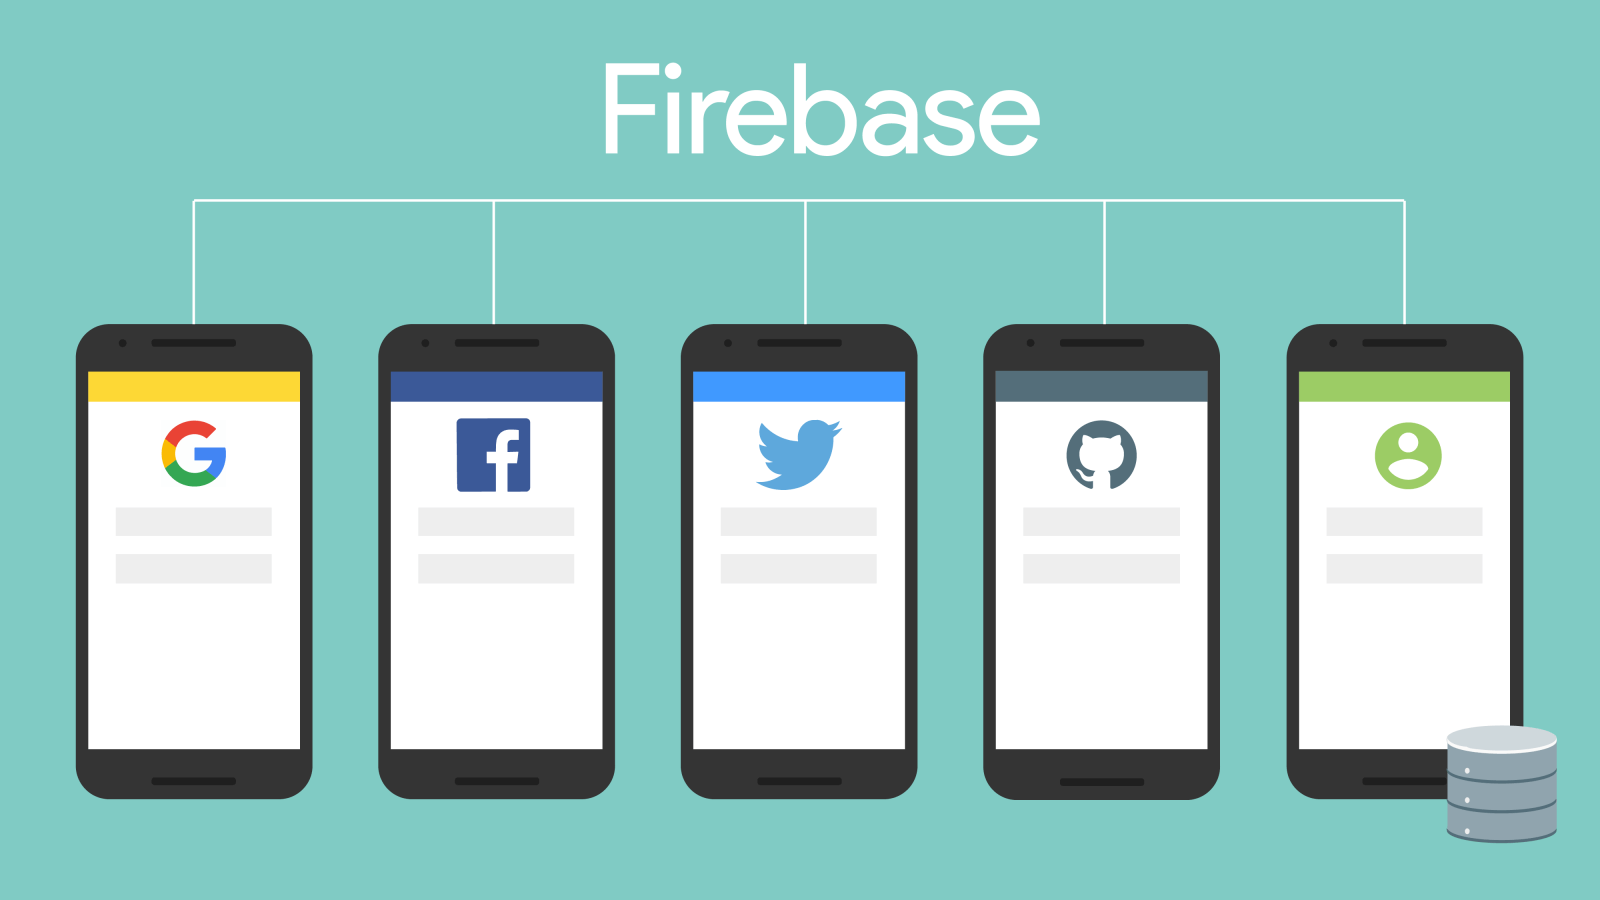
\includegraphics[width=0.45\textwidth,height=\textheight]{media/e1401/image4.png}}

\end {centerimageenv}

\begin {smalltextenv}

Imagen 2 - \textbf{Fuente:} \emph{\href{https://firebase.google.com/docs/auth/images/auth-providers.png}{Firebase Google}}

\end {smalltextenv}

Otro gran ejemplo es \textbf{Admob}, este es uno de los más utilizados por las aplicaciones gratuitas de la red, nos permite colocar publicidad de manera amigable con el fin de mantener un ingreso capaz de financiar el desarrollo para programadores o aplicaciones principiantes. Dependiendo de la región donde se utilice tu aplicación Firebase manejara junto con Google los Analytics necesarios para tus usuarios.

Ahora que has manejado funcionalidades para ti como desarrollador, te presentamos otros tipos de servicios que harán que la experiencia de usuario sea exitosa y amigable, lo cual atrae a más clientes potenciales. Uno de los más grandes problemas al desarrollar es el manejo de \textbf{Notificaciones}, no por su complejidad, sino porque con cada lenguaje debemos encontrar las herramientas específicas para mostrar de manera amigable mensajes que les brinden advertencias a los usuarios. Con Firebase esto deja de ser un problema como tal y pasa a ser un paso simple, podremos gestionar notificaciones con simples parámetros y Firebase se encargara del resto. Otro gran problema que se presenta con los usuarios es la interfaz ¿Cómo manejar de manera eficiente como se le presenta nuestra aplicación a los usuarios desde cualquier dispositivo? Con \textbf{Enlaces dinámicos} de Firebase nuestra aplicación se adaptaría a cada dispositivo, esto lo podemos gestionar mientras el desarrollo de nuestro programa se encuentra en marcha. Todo esto claro con la dirección y guía de Firebase, esto de manera estandarizada.

\hypertarget{muxe1s-que-una-herramienta-un-ambiente}{%
\section{Más que una herramienta, un ambiente}\label{muxe1s-que-una-herramienta-un-ambiente}}

Aunque Firebase sea más conocido como un conjunto de herramientas para desarrolladores también nos ofrece el servicio de \textbf{Hosting,} un ambiente de trabajo. Tal y como su nombre nos lo indica este servicio nos permite colocar nuestra aplicación bajo el cargo de Firebase y funcionalidades Cloud. Esto en una plataforma que nos ofrece seguridad, protocolos, alta escalabilidad y alta disponibilidad, todo lo que nos ofrecería otro servicio de la nube para montar nuestro programa. No está de más mencionar que cualquier tipo de software puede ser adquirir este servicio, ¡No existen limitantes! Ya sea que tu aplicación esté realizada con JavasScript, Python, aplicaciones de IOS, Android, entre otros, el SDK de Firebase siempre estará disponible. Otra gran ventaja de utilizar este servicio es la facilidad de desarrollar sitios estáticos o sitios prefabricados, es tan simple como instalar la herramienta de Firebase CLI, configurar tu proyecto dependiendo de tus necesidades e implementarlo. Tres simples pasos para soluciones eficientes.

Todo esto también incluye la replicación del resguardo de tu información y aplicación alrededor del mundo ``ver imagen 3'', dándole una latencia y consistencia de conexión de buena calidad desde cualquier punto.

\begin {centerimageenv}

\href{https://medium.com/evenbit/gateway-to-firebase-hosting-dda81e83fcfa}{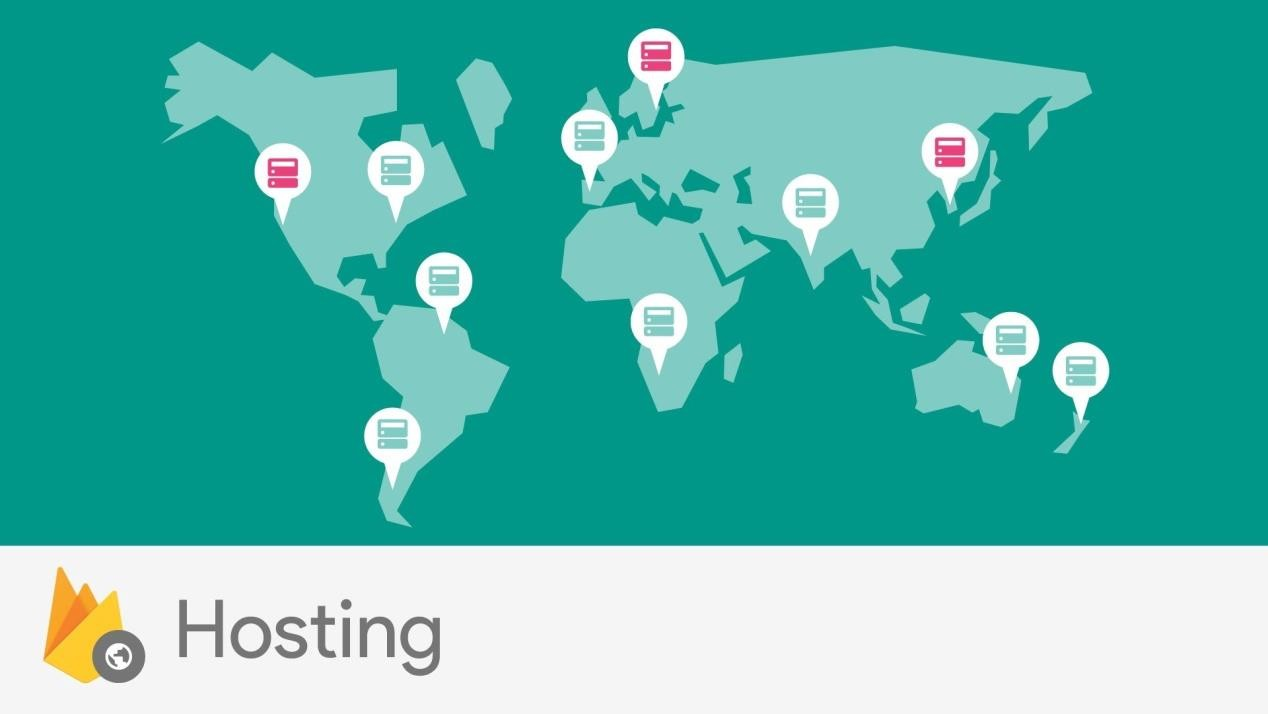
\includegraphics{media/e1401/image5.jpeg}}

\end {centerimageenv}

\begin {smalltextenv}

Imagen 3 - \textbf{Fuente:} \emph{\href{https://medium.com/evenbit/gateway-to-firebase-hosting-dda81e83fcfa}{Firebase Google}}

\end {smalltextenv}

\hypertarget{como-testimonio-personal}{%
\section{Como testimonio personal}\label{como-testimonio-personal}}

Todos estos servicios y más al alcance de cualquier desarrollador en el planeta no pueden ser del todo gratuitos ¿verdad? Déjame decirte que algunos si lo son y dependerán de la magnitud del uso de los mismos. Firebase nos dejará experimentar y vivir la experiencia de utilizar muchas de sus herramientas de manera gratuita, solo deberemos formar parte de la familia de Google y listo. Dentro de Firebase podremos encontrar todo tipo de guías junto con tutoriales, todo lo necesario para que empieces a trabajar y desarrollar tus ideas.

Para animarte aún más a probar esta grandiosa herramienta déjame contarte que en menos de un mes se logró construir un proyecto de IOT con hardware y software desde cero que incluía una base de datos NoSql, donde se almacenaba datos de manera masiva, software desarrollado en python, Arduino y Android, un circuito encapsulado y amigable que brindaba el control de tanques de almacenamiento de agua potable. Un proyecto totalmente viable sin invertir un solo dólar, gracias a los servicios que nos proporcionó Firebase. Así que no lo pienses más y únete a la comunidad y se parte del futuro de desarrollo de aplicaciones.

\hypertarget{conclusiones}{%
\section{Conclusiones:}\label{conclusiones}}

\begin{itemize}
\item
  Firebase es un conjunto de herramientas que ayudan a desarrollar soluciones de alta calidad y eficiencia bajo los estándares y responsabilidad de Google.
\item
  Los servicios de Firebase están guiados para que cualquier persona con conocimientos básicos de desarrollo de software pueda realizar infinidad de proyectos tecnológicos.
\item
  Al ser servicios de Google estos nos brindan soporte, mantenimiento y guía de calidad en cualquier momento, así que los protocolos y aplicaciones agregadas que se utilicen serán de total confianza y totalmente eficientes.
\end{itemize}

\hypertarget{referencias-bibliograficas}{%
\section{Referencias bibliográficas:}\label{referencias-bibliograficas}}

\begin{itemize}
\item
  \href{https://firebase.google.com}{Firebase google. Una plataforma integral para desarrollo de dispositivos móviles} (04/2019)
\item
  \href{https://firebase.google.com/docs/guides/}{Firebase Google. Guía de Firebase} (04/2019)
\item
  \href{https://medium.com/evenbit/gateway-to-firebase-hosting-dda81e83fcfa}{Dennis Alund (02/2017) Gateway to Firebase: Hosting} (04/2019)
\item
  \href{https://openwebinars.net/blog/que-es-firebase-de-google/}{Miguh Ruiz (08/2017) ¿Qué es Firebase de Google?} (04/2019)
\end{itemize}

\end {multicols}

\begin {centerimageenv}


\includegraphics[width=0.9\textwidth,height=\textheight]{media/e14publi/04.png}

\end {centerimageenv}

\begin {centerimageenv}


\includegraphics[width=0.9\textwidth,height=\textheight]{media/e14publi/20.jpg}

\end {centerimageenv}

\begin {centerimageenv}


\includegraphics[width=0.9\textwidth,height=\textheight]{media/e14publi/21.jpg}

\end {centerimageenv}

\titleformat{\chapter}[display]{\formatchapter}{\labelchapter}{\sepchapter}{\beforecodechapter#1\beforecodechapterparttwo}

\titlespacing*{\chapter} {\leftchapter}{\beforesepchapter}{\afterchapter}

\titleformat{\section}[block]{\formatsection}{\labelsection}{\sepsection}{\beforecodesection#1}

\hypertarget{article02}{%
\chapter{Edge Computing}\label{article02}}

\begin {multicols}{2}

\BeginKnitrBlock{photobiography3}{media/e1402/image2.jpeg}
\textbf{Esteban David Alvarez Bor}\\
\href{mailto:davix93a@gmail.com}{\nolinkurl{davix93a@gmail.com}}

\medskip

Estudiante de Ingeniería en Ciencias y Sistemas - USAC

\medskip

Palabras Clave: Cloud Computing, Edge Computing, AWS, Cloud, IoT, Latencia.
\EndKnitrBlock{photobiography3}

Edge Computing es un concepto relativamente nuevo, surge a partir del concepto de Cloud Computing, en el cual se intenta acercar el almacenamiento y procesamiento a la fuente de los datos, para no enviar toda la data a un servidor remoto en la nube o a un sistema centralizado que procese la misma. Esto representa un cambio en la arquitectura provista por los sistemas tradicionales de Internet de las cosas, que utilizan Cloud Computing con la finalidad de proveer a sistemas la capacidad de procesamiento de datos, casi en tiempo real, mejorando así el nivel de respuesta de aquellos sistemas que su información es de suma importancia, como dispositivos médicos, industriales y muy recientemente en vehículos autónomos.

IEEE define Internet de las cosas como \emph{``Un campo de aplicación que integra campos tecnológicos y sociales''} . La firma de análisis Gartner nos proporciona una definición más extensa de la que podemos extraer "\emph{IoT es una red dedicada de objetos físicos con tecnología integrada que mide y comunica la interacción entre factores internos y externos"} , además dentro de esta definición nos menciona un factor muy importante, como la data capturada permite a las compañías aprender el comportamiento y uso de sus sistemas, permitiéndoles tomar una serie de acciones preventivas o mejorar sus procesos de negocios.

Si consideramos un sistema de Internet de las Cosas, desarrollado actualmente bajo el concepto de Cloud Computing, el cual Amazon Web Services define como ``\emph{La entrega a pedido de poder de cómputo, almacenamiento, aplicaciones y recursos de TI a través de una plataforma en la nube en internet con precios basados en el consumo.}'', hay dos factores clave que debemos considerar al momento de evaluar el grado de importancia como lo son la velocidad de procesamiento y el tiempo de respuesta. Aunque hay sistemas que se acoplan perfectamente a un entorno en la nube como en el caso de sistemas de domótica, hay otros como en el caso de sistemas de Internet de las Cosas del sector médico, bancario e industrial, que requieren de un grado superior de procesamiento y respuesta debido a la sensibilidad de la información que maneja, y factores como la conexión a internet, el lugar en donde se despliega el servidor, puede influir en los factores mencionados anteriormente.

Para estos sistemas especiales, en los cuales la velocidad de procesamiento y respuesta son esenciales e indispensables, surge el concepto de Edge Computing o Cómputo en el borde, en el cual, su premisa es acercar tanto como sea posible el almacenamiento y procesamiento de la data al dispositivo que la genera, con el propósito de eliminar la latencia en estos procesos. Este concepto toma fuerza cuando analizamos la cantidad masiva de datos generada por un dispositivo de Internet de las Cosas, y el tiempo considerable que a esta le toma al ser enviada y analizada a través de la red, cuando decisiones como detener una línea de ensamblaje, reactivar una planta eléctrica o incluso diagnosticar mediante un monitor biométrico en el cual milisegundos pueden ser valiosos.

\begin {centerimageenv}

\href{https://www.cisco.com/c/en/us/solutions/internet-of-things/edge-computing-architecture/_jcr_content/Grid/article_bc26/layout-article/full_c27d/Full/text_floating_image_/image.img.png/1531803020568.png}{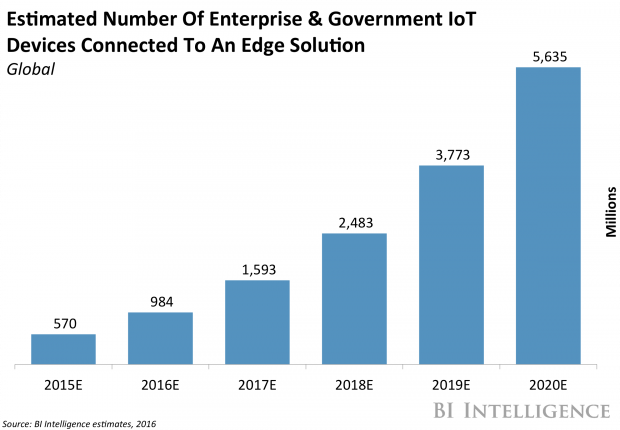
\includegraphics[width=0.45\textwidth,height=\textheight]{media/e1402/image3.png}}

\end {centerimageenv}

\begin {smalltextenv}

Imagen 1 - \textbf{Fuente:} \emph{\href{https://www.cisco.com/c/en/us/solutions/internet-of-things/edge-computing-architecture/_jcr_content/Grid/article_bc26/layout-article/full_c27d/Full/text_floating_image_/image.img.png/1531803020568.png}{BI Intelligence}}

\end {smalltextenv}

Un estudio realizado por BI Intelligence pronosticó un estimado de 5.635 mil millones de dispositivos conectados bajo el modelo de Edge Computing para el año 2020 tanto en sectores del gobierno como de la industria.

Para poder entender mejor el concepto de Edge Computing, se creó el concepto de Fog Computing o Cómputo en la niebla, donde podemos hacer la analogía con una nube física, en la cual la niebla es la parte exterior o borde de ella. Mas formalmente se define como ``\emph{Una infraestructura de computo descentralizada en la cual tanto la data, cómputo, almacenamiento y aplicaciones están localizadas en un lugar intermedio de la fuente de datos y la nube.}''. Este concepto define el estándar de como Edge Computing debe trabajar para facilitar las operaciones del modelo.

\begin {centerimageenv}

\href{https://cdn.ttgtmedia.com/rms/onlineImages/edgecomputing.jpg}{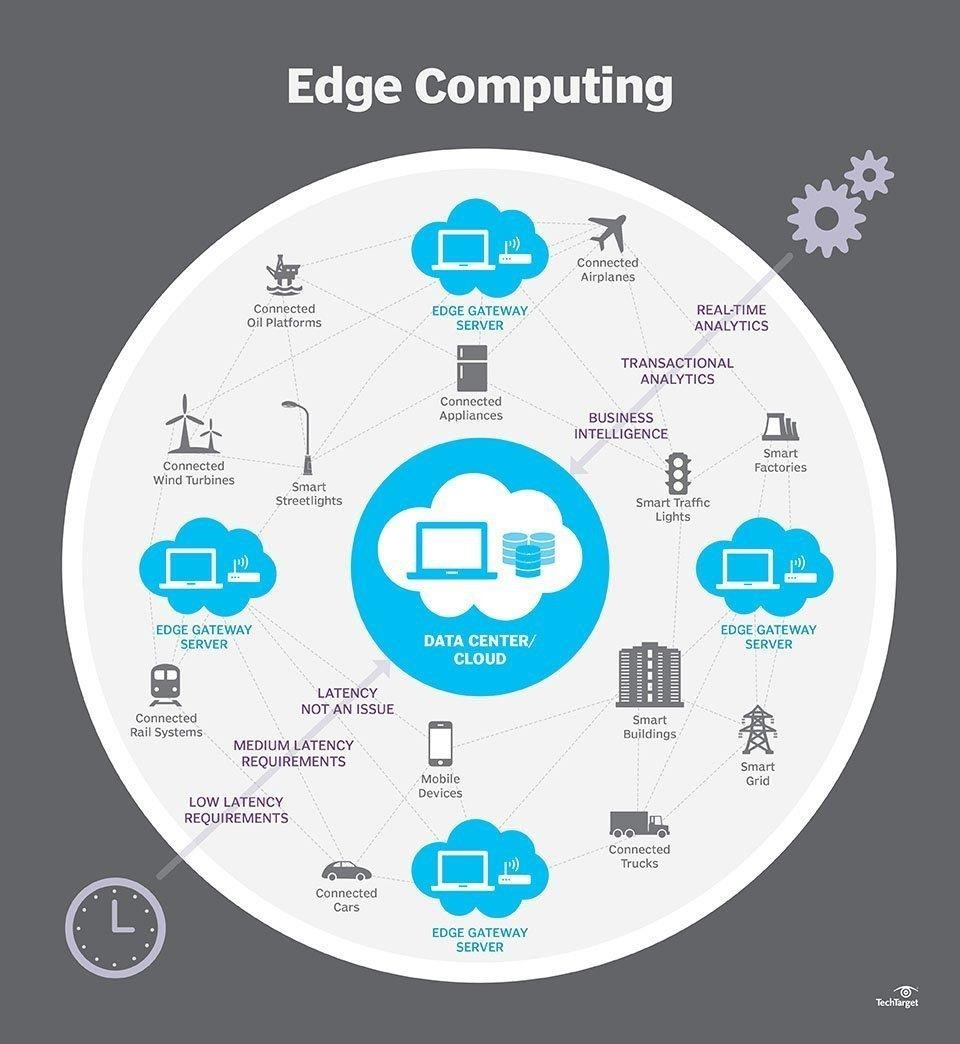
\includegraphics[width=0.45\textwidth,height=\textheight]{media/e1402/image4.jpeg}}

\end {centerimageenv}

\begin {smalltextenv}

Imagen 2 - \textbf{Fuente:} \emph{\href{https://cdn.ttgtmedia.com/rms/onlineImages/edgecomputing.jpg}{TechTarget}}

\end {smalltextenv}

En la actualidad, el ejemplo más acertado del uso de Edge Computing es en los sistemas utilizados por los vehículos autónomos. Estos vehículos, cuentan con un amplio conjunto de sensores los cuales recolectan grandes cantidades de información como velocidad, distancia, ruta, detección de objetos entre otros.

Un artículo escrito por Kathy Winter, para Intel Newsroom, indica que se estima una cantidad de cuatro terabytes de datos recolectados por un vehículo autónomo en un solo día. Estos datos recolectados requieren de un rápido procesamiento y respuesta debido a que se espera una conducción lo más óptima y segura posible. Aquí entra Edge Computing agilizando el procesamiento de los datos generando resultados en tiempo real para un sistema complejo.

\begin {centerimageenv}

\href{https://simplecore.intel.com/newsroom/wp-content/uploads/sites/11/2017/04/Autonomous-Vheicle-Data-1000x500.jpg}{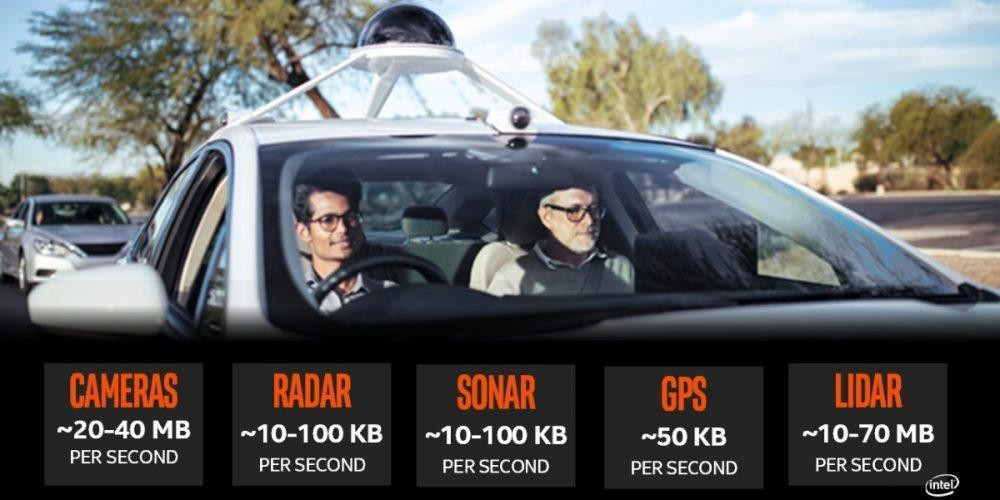
\includegraphics[width=0.45\textwidth,height=\textheight]{media/e1402/image5.jpeg}}

\end {centerimageenv}

\begin {smalltextenv}

Imagen 3 - \textbf{Fuente:} \emph{\href{https://simplecore.intel.com/newsroom/wp-content/uploads/sites/11/2017/04/Autonomous-Vheicle-Data-1000x500.jpg}{Intel}}

\end {smalltextenv}

Plataformas de Cloud Computing han desarrollado servicios capaces de dar solución a la problemática de latencia en despliegues totalmente en la nube, Amazon Web Services proporciona un servicio llamado Lambda@Edge, el cual tiene la finalidad de acercar la ejecución de código al usuario, mejorando el rendimiento y reduciendo la latencia, sin la necesidad de administrar infraestructura en distintas partes del mundo. IoT Greengrass es otro servicio proporcionado por AWS permitiendo una interacción a nivel local en función de los datos generados y el uso de la nube para tareas administrativas, análisis y almacenamiento duradero.

\hypertarget{conclusiones-1}{%
\section{Conclusiones:}\label{conclusiones-1}}

\begin{itemize}
\item
  Edge Computing busca reducir la latencia acercando el procesamiento de los datos lo más cerca del lugar de donde se originan.
\item
  Fog Computing define el estándar de como Edge Computing debería trabajar.
\item
  El uso de Edge Computing depende de las características de nuestro sistema, la velocidad de procesamiento y velocidad de respuesta requerida para satisfacer las necesidades de este.
\item
  Sistemas de información vital o de suma importancia son los principales en acoplarse al modelo de Edge Computing.
\end{itemize}

\hypertarget{referencias-bibliograficas-1}{%
\section{Referencias bibliográficas:}\label{referencias-bibliograficas-1}}

\begin{itemize}
\item
  \href{https://iot.ieee.org/images/files/pdf/IEEE_IoT_Towards_Definition_Internet_of_Th\%20\%5B\%20ings_Revision1_27MAY15.pdf}{IEEE. (2015). towards a definition of the Internet of Things (IoT). 28/03/19, de IEEE}
\item
  \href{https://www.gartner.com/imagesrv/books/iot/iotEbook_digital.pdf\%5B}{Gartner. (2017). Leading the IoT. 28/03/19, de Gartner}
\item
  \href{\%5Bhttps://docs.aws.amazon.com/es_es/aws-technical-content/latest/aws-\%20overview/what-is-cloud-computing.html}{Amazon Web Services. (2019). What it Cloud Computing? 28/03/19, de AWS}
\item
  \href{https://internetofthingsagenda.techtarget.com/definition/fog-computing-fogging}{Margaret Rouse. (2019). Fog computing. 28/03/19, de IoT Agenda, TechTarget fogging})
\item
  \href{https://aws.amazon.com/es/lambda/edge/\%5B}{Amazon Web Services. (2019). Lambda@Edge. 28/03/19, de AWS}
\item
  \href{\%5Bhttps://aws.amazon.com/es/greengrass/}{Amazon Web Services. (2019). AWS IoT Greengrass. 28/03/19, de AWS}
\item
  \href{https://www.cisco.com/c/en/us/solutions/enterprise-networks/edge-\%20\%5Bcomputing.html}{David Linthicum. Edge computing vs.~fog computing: Definitions and enterprise uses. 28/03/19, de Cisco}
\item
  \href{https://www.cisco.com/c/en/us/solutions/internet-of-things/edge-computing-architecture.html}{Lauren Horwitz. Connected devices push business to the edge (edge computing architecture that is). 28/03/19, de Cisco}
\item
  \href{https://newsroom.intel.com/editorials/self-driving-cars-big-meaning-behind-one-number-4-terabytes/}{Kathy Winter. (2017). for self-driving cars, there's big meaning behind one big number: 4 terabytes. 28/03/19, de Intel Newsroom}
\end{itemize}

\end {multicols}

\begin {centerimageenv}


\includegraphics[width=1\textwidth,height=\textheight]{media/e14publi/03.jpg}

\end {centerimageenv}

\begin {centerimageenv}

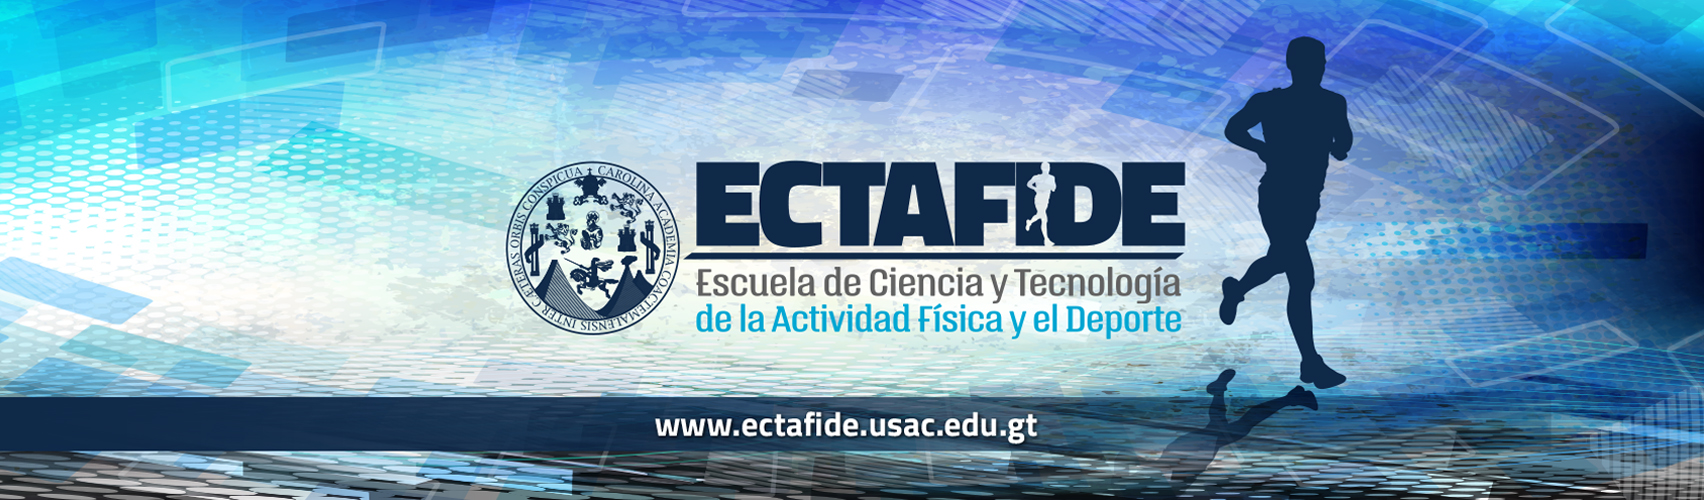
\includegraphics[width=1\textwidth,height=\textheight]{media/e14publi/05.jpg}

\end {centerimageenv}

\begin {centerimageenv}


\includegraphics[width=1\textwidth,height=\textheight]{media/e14publi/06.jpg}

\end {centerimageenv}

\titleformat{\chapter}[display]{\formatchapter}{\labelchapter}{\sepchapter}{\beforecodechapter#1\beforecodechapterparttwo}

\titlespacing*{\chapter} {\leftchapter}{\beforesepchapter}{\afterchapter}

\titleformat{\section}[block]{\formatsection}{\labelsection}{\sepsection}{\beforecodesection#1}

\hypertarget{article03}{%
\chapter{Flutter: el presente de las aplicaciones móviles}\label{article03}}

\begin {multicols}{2}

\BeginKnitrBlock{photobiography3}{media/e1403/image1.jpeg}
*Fabio César De Paz Vásquez**\\
\href{mailto:fabiodepazv@gmail.com}{\nolinkurl{fabiodepazv@gmail.com}}

\medskip

Estudiante de Ingeniería en Ciencias y Sistemas - USAC

\medskip

Palabras Clave: Desarrollo de aplicaciones híbridas, Dart, Flutter, Google.
\EndKnitrBlock{photobiography3}

En el contexto de aplicaciones móviles, tomar una decisión sobre qué grupo de herramientas utilizar para crear aplicaciones nuevas, es una decisión bastante compleja, ya que, al existir distintos sistemas operativos, se requiere que las aplicaciones puedan ejecutarse de manera correcta en cualquiera de estas. Como consecuencia a esto, algunas personas tienden a inclinarse por implementar sus nuevos proyectos utilizando lo que se conoce como aplicaciones móviles híbridas. Para poder explicar y adentrarse en esta pequeña parte del universo del desarrollo, es necesario presentar contexto respecto a esto.

\begin {centerimageenv}

\href{https://upload.wikimedia.org/wikipedia/commons/0/0e/Fotos_produzidas_pelo_Senado_\%2830554309793\%29.jpg}{
\includegraphics[width=0.45\textwidth,height=\textheight]{media/e1403/image3.jpeg}}

\end {centerimageenv}

\begin {smalltextenv}

Imagen 1 - \textbf{Fuente:} \emph{\href{https://upload.wikimedia.org/wikipedia/commons/0/0e/Fotos_produzidas_pelo_Senado_\%2830554309793\%29.jpg}{Wikipedia, User: Senado Federal}}

\end {smalltextenv}

Para el desarrollo móvil, se cuenta con tres distintas alternativas a elegir, como se describen a continuación:

\begin{itemize}
\item
  \textbf{Desarrollo nativo:} A manera de simplificar su descripción, puede describirse como aquellas aplicaciones que son desarrolladas utilizando específicamente el lenguaje de la plataforma donde se ejecutan, por ejemplo: JAVA para Android o Swift para iOS. Esto podría complicar la situación de poder publicar la misma aplicación en distintas plataformas, ya que estas son excluyentes con los otros lenguajes nativos, lo que trae consigo el hecho de tener que realizar doble trabajo si se quisiera desarrollar para varias plataformas de manera nativa. Entonces, ¿por qué razones desarrollar de manera nativa?

  \begin{itemize}
  \item
    Permiten mejorar el performance de la aplicación.
  \item
    El look \& feel que se logra generar es óptimo y su fluidez es evidente.
  \item
    Es posible acceder a todos los componentes del dispositivo, como los sensores y actuadores.
  \end{itemize}
\item
  Estas razones parecen ser convincentes para que los desarrolladores opten por esta alternativa, pero si se quiere realizar implementaciones de manera masiva e invirtiendo menos recursos, esta termina siendo una opción compleja y costosa, debido a esto han surgido las siguientes formas de implementación.
\item
  \textbf{Desarrollo híbrido:} Se trata de aplicaciones que se desarrollan implementando estándares de aplicaciones web, mediante HTML, CSS y JavaScript, que finalmente es renderizado en el teléfono mediante el uso de un framework específico (como lo puede ser PhoneGap, Ionic o Cordova). Esta parece ser una opción bastante viable, ya que realizando un único desarrollo es posible visualizar y ejecutar las aplicaciones tanto en ambientes web, como Android y iOS. Recientemente, este método es utilizado por muchas empresas y programadores a nivel mundial, ya que se ahorran el tiempo de desarrollo y reducen la complejidad del código, simplificándolo a una misma sintaxis y compilación. Estos frameworks ofrecen a los desarrolladores el acceso a funcionalidades nativas a través de ellos, pero como muchas cosas en el mundo, existen sus limitantes. Esto no quiere decir que sea de mala calidad, sino que de cierta forma no tienen acceso a todos los componentes del teléfono y además la fluidez visual no será la misma, debido a la existencia de una capa intermedia que se encarga de renderizar las vistas.
\item
  \textbf{Desarrollo generado o bridged:} Se trata del desarrollo a través de distintos frameworks que ofrecen su sintaxis y características para escribir el código, pero finalmente estas se encargan de traducir estas instrucciones hacia instrucciones del lenguaje nativo de la plataforma sobre la cual se ejecutan.
\end{itemize}

Teniendo esto en mente, es posible adentrarse un poco en lo que es Flutter\textsuperscript{2}. Se trata de un framework de desarrollo de aplicaciones móviles creado por Google, teniendo su primer reléase al público en general en mayo de 2017, pero, presentando su primer reléase estable el 22 de febrero de 2019. Flutter se encuentra optimizado para crear aplicaciones tanto Android, como iOS y de manera novedosa, incluyen el sistema operativo en desarrollo propio de Google, Google Fuchsia.

\begin {centerimageenv}

\href{https://flutter.io/images/flutter-mark-square-100.png}{
\includegraphics[width=0.45\textwidth,height=\textheight]{media/e1403/image4.png}}

\end {centerimageenv}

\begin {smalltextenv}

Imagen 2 - \textbf{Fuente:} \emph{\href{https://flutter.io/images/flutter-mark-square-100.png}{Flutter}}

\end {smalltextenv}

Una de las características ofrecidas por Flutter, es que como código fuente utiliza el lenguaje Dart, que es un lenguaje de propósito general, también creado por Google y que se utiliza para construir aplicaciones en distintas plataformas, como web, de servidores, de escritorio e incluso aplicaciones móviles. Dentro de sus atributos es posible mencionar que se trata de un lenguaje orientado a objetos, que utiliza definición por clases, cuenta con su propio Garbage Collector y su sintaxis es similar al lenguaje C. Para describir de mejor manera Flutter, es necesario describir sus componentes:

\begin{itemize}
\item
  \textbf{Flutter engine:} Es el core de Flutter, se encuentra desarrollado en C++ y proporciona soporte bastante amplio a bajo nivel del dispositivo, lo que permite el acceso al hardware del dispositivo. Se vincula de manera directa con los SDK de Android y de iOS.
\item
  \textbf{Foundation library:} Son componentes escritos en Dart, que pone a disposición de los programadores, para que puedan reutilizarlo, se trata de clases y funciones básicas que son requeridas para ejecutar Flutter, un ejemplo de esto serían las APIs utilizadas para hacer llamadas a su engine.
\item
  \textbf{Widgets:} El desarrollo de la interfaz de Flutter se basa en widgets. Cada componente visual que se puede apreciar es un widget. Dentro de las ventajas de Flutter, está en que es posible combinar distintos widgets con el objetivo de generar nuevas combinaciones, tal como las indique o requiera el programador. Dentro de los widgets se ofrece de manera original, los diseños visuales de Material Design (usado por Android) y de Cupertino (diseños usados por iOS).
\end{itemize}

Una vez descrito qué es Flutter y cómo es su arquitectura principal, el lector podría pensar: ¿por qué usar Flutter? ¿Por qué no simplemente utilizar algún otro framework de renderización web?\textsuperscript{1}. Pues existen muchas respuestas a estas preguntas, tales como el soporte de la comunidad, el auge de este nuevo framework, lo cual se puede notar en su alta demanda\textsuperscript{3} mediante la \textbf{imagen 3}. Otro motivo, es el respaldo que ofrece Google, una empresa de gran trayectoria y actualización constante, quienes además brindan soporte técnico, implementación de nuevas características, y la frecuente reparación de posibles bugs. Todo esto suena bien, pero va un poco por encima de lo que es en realidad la ventaja principal de Flutter, por lo que se requiere una especificación más técnica: Flutter no utiliza un render de tipo web, en cambio, utiliza un canvas optimizado, en el que renderiza sus propios widgets con llamadas al sistema a bajo nivel, esto mediante la utilización de Dart.

Esto permite tener acceso a la mayor cantidad de hardware del dispositivo (sensores, cámaras, actuadores), teniendo una renderización visual casi natural que es compatible con los sistemas operativos antes mencionados. Todas estas características dejan a Flutter como un fuerte candidato a considerar, sin mencionar que ya está siendo implementado por Google, Google ADs, Tencent, y el gigante de ventas mundiales Alibaba, quien recientemente implementó Flutter para su aplicación móvil, y que cuenta con más de 50 millones de descargas.

\begin {centerimageenv}

\href{https://1.bp.blogspot.com/-dAf9QhjGWiU/W6AvC4RRDoI/AAAAAAAAGC8/-LxXBV8saNA4smHV5shyRhkfqUHpWDq_wCLcBGAs/s1600/pasted\%2Bimage\%2B0\%2B\%252813\%2529image4.png}{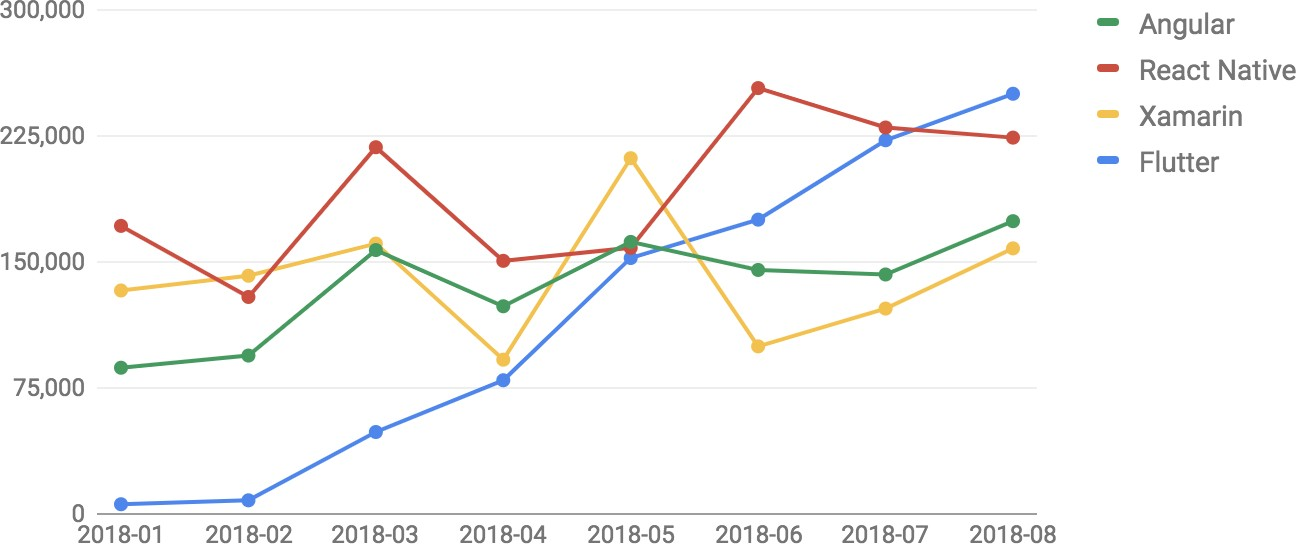
\includegraphics[width=0.45\textwidth,height=\textheight]{media/e1403/image5.jpeg}}

\end {centerimageenv}

\begin {smalltextenv}

Imagen 3 - \textbf{Fuente:} \emph{\href{https://1.bp.blogspot.com/-dAf9QhjGWiU/W6AvC4RRDoI/AAAAAAAAGC8/-LxXBV8saNA4smHV5shyRhkfqUHpWDq_wCLcBGAs/s1600/pasted\%2Bimage\%2B0\%2B\%252813\%2529image4.png}{Google}}

\end {smalltextenv}

\hypertarget{conclusiones-2}{%
\section{Conclusiones:}\label{conclusiones-2}}

\begin{itemize}
\item
  El hecho de decidir entre qué tipo de implementación realizar, ya sea nativa, híbrida o generada, es una decisión importante que deben tomar los desarrolladores y encargados de sistemas, debiendo evaluar sus características ofrecidas y las necesidades que deben cubrir.
\item
  Flutter es un framework de desarrollo potente, de gran auge que permite a los programadores, simplificar el tiempo y complejidad del proceso de escritura de código.
\item
  La forma de generar aplicaciones a través de Flutter es lo más similar a una aplicación nativa, guardando los accesos a hardware y la fluidez de las interfaces gráficas, permitiendo además la generación de aplicaciones multiplataforma en un único código fuente.
\end{itemize}

\hypertarget{referencias-bibliograficas-2}{%
\section{Referencias bibliográficas:}\label{referencias-bibliograficas-2}}

\begin{itemize}
\item
  \href{https://www.northware.mx/desarrollo-de-aplicaciones-moviles-hibridas/}{Guillermo Martínez. Desarrollo de aplicaciones móviles híbridas ¿Me conviene?}(12/09/2017)
\item
  \href{https://medium.com/asos-techblog/flutter-vs-react-native-for-ios-android-app-development-c41b4e038db9}{Marco Bellinaso. Flutter: the good, the bad and the ugly} (23/11/2018)
\item
  \href{https://developers.googleblog.com/2018/09/flutter-release-preview-2-pixel-perfect.html}{Flutter Team. Flutter Release Preview 2: Pixel-Perfect on iOS} (19/09/2019)
\end{itemize}

\end {multicols}

\begin {centerimageenv}


\includegraphics[width=1\textwidth,height=\textheight]{media/e14publi/07.jpg}

\end {centerimageenv}

\begin {centerimageenv}

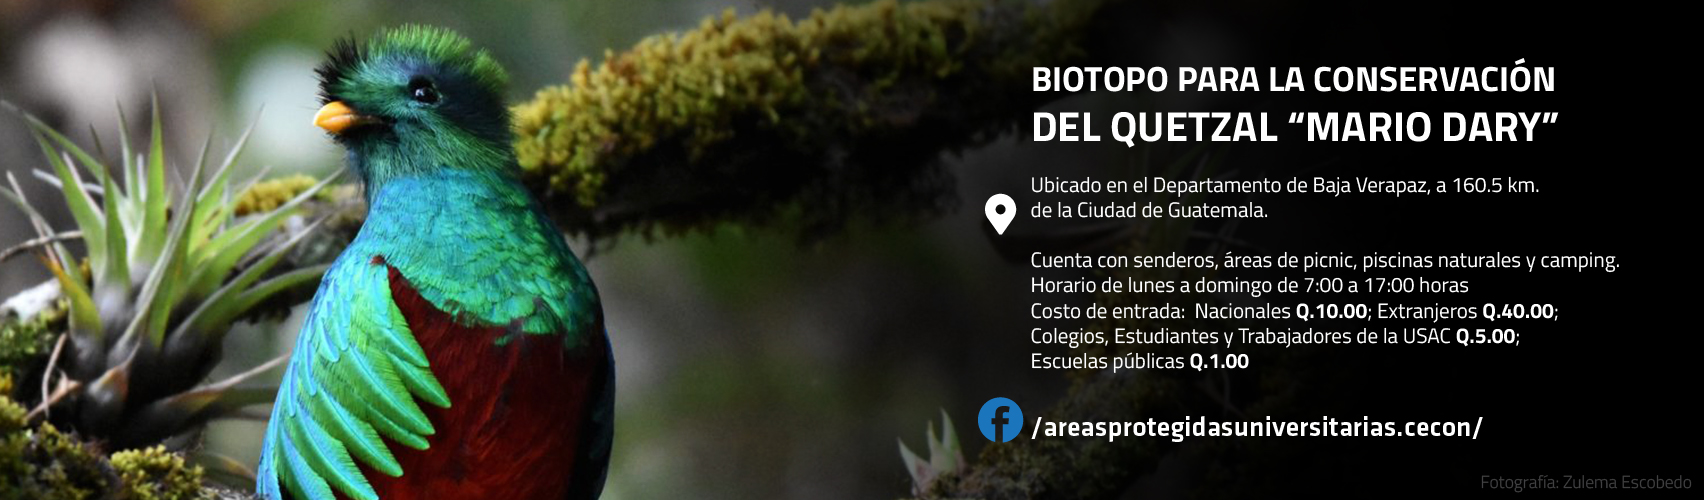
\includegraphics[width=1\textwidth,height=\textheight]{media/e14publi/08.jpg}

\end {centerimageenv}

\titleformat{\chapter}[display]{\formatchapter}{\labelchapter}{\sepchapter}{\beforecodechapter#1\beforecodechapterparttwo}

\titlespacing*{\chapter} {\leftchapter}{\beforesepchapter}{\afterchapter}

\titleformat{\section}[block]{\formatsection}{\labelsection}{\sepsection}{\beforecodesection#1}

\hypertarget{article04}{%
\chapter{Computación paralela a través de CUDA}\label{article04}}

\begin {multicols}{2}

\BeginKnitrBlock{photobiography3}{media/e1404/image1.jpeg}
\textbf{Erick Roberto Tejaxún Xicón}\\
\href{mailto:erickteja@gmail.com}{\nolinkurl{erickteja@gmail.com}}

\medskip

Estudiante de Ingeniería en Ciencias y Sistemas - USAC\\

\medskip

Palabras Clave: CUDA, Kernel, Paralelismo, Multicore, Instrucción, GPU.
\EndKnitrBlock{photobiography3}

\hypertarget{computaciuxf3n-paralela}{%
\section{Computación paralela}\label{computaciuxf3n-paralela}}

La computación paralela hace referencia a la capacidad de poder realizar varias tareas al mismo tiempo. Esto aplicado a las ciencias de la computación se ha estado trabajando desde hace muchos años, casi al mismo tiempo que el inicio de la computación moderna.

Pero, ¿para qué aplicar computación paralela? La computación paralela tiene como objetivo acelerar una aplicación, es decir, reducir el tiempo de procesamiento. Por lo cual el motivo que ha traído consigo la búsqueda de un estándar para el uso de computación paralela ha sido ese, de tener problemas que requieren gran cantidad de capacidad y tiempo de cómputo. Por ejemplo, un problema de simulación de colisiones de partículas, utilizando un algoritmo secuencial y usando un solo procesador podría llevar años en su finalización.

En un principio, cuando se contaba con una computadora con un único procesador, el paralelis-
mo se aplicó creando una red de computadoras dentro de las cuales se pudiera trabajar en un mismo problema. Es decir, cada computadora conectada a esta red, tendría la tarea de trabajar sobre una porción del problema. Minimizando así el tiempo de computación para la solución del problema. Esto se sigue aplicando hoy en día y podemos encontrar sitios especializados en este tema, que llevan el recuento y el listado de las supercomputadoras más potentes del mundo como top500.org.

\begin {centerimageenv}

\href{https://www.top500.org/lists/2018/11/}{
\includegraphics[width=0.45\textwidth,height=\textheight]{media/e1404/image3.jpeg}}

\end {centerimageenv}

\begin {smalltextenv}

Imagen 1 - \textbf{Fuente:} \emph{\href{https://www.top500.org/lists/2018/11/}{Top500.org}}

\end {smalltextenv}

Como vemos en la ilustración anterior tomada de la página Top500.org, las supercomputadoras en la actualidad cuentan con millones de núcleos que pueden trabajar en conjunto y generar un throughput en el orden de miles de Teraflops por segundo. Cabe mencionar que estas supercomputa-
doras están en centros de investigación en países del primer mundo.

A través del tiempo, la computación paralela ha sido un tema estudiado de sobremanera ya que tiene muchas aplicaciones en cualquier ámbito. Quizá en algún futuro se pueda contar en nuestra escuela con un curso sobre el tema como el que se cuenta ya en la Escuela de Ciencias Físicas y Matemáticas el cual tiene un enfoque científico donde se tratan de resolver problemas de sistemas dinámicos, corridas de método Montecarlo entre otros.

Se han diseñado diferentes arquitecturas de memoria para la computación paralela. Esto debido a que el principio de esta es que se debe de trabajar sobre un mismo conjunto de datos que conforman todo el problema en sí. Entre estas arquitecturas tenemos la arquitectura de acceso uniforme a memoria (UMA por sus siglas en inglés), arquitectura de acceso no uniforme a memoria (NUMA por sus siglas en inglés).

Dentro del paralelismo a nivel de datos existen cuatro técnicas básicas las cuales son: única instrucción, múltiple datos (SIMD siglas en inglés). Múltiple instrucciones, múltiple datos (MIMD), única instrucción, un dato (SISD) y múltiple instrucción, un dato (MISD). La más utilizada es la de única instrucción, múltiples datos.

\hypertarget{quuxe9-es-cuda}{%
\section{¿Qué es CUDA?}\label{quuxe9-es-cuda}}

CUDA (Arquitectura unificada de dispositivos de cómputo) es una arquitectura de procesamiento en paralelo creada por la empresa especializada en tarjetas gráficas Nvidia, en la que se trata de aprovechar la capacidad y potencia de sus GPU (Unidad de procesamiento gráfico) como una alternativa al procesamiento en CPU's tradicionales.

CUDA es una tecnología basada tanto en hardware como en software. En hardware al hacer que la arquitectura de sus tarjetas gráficas estén preparadas para poder explotar el paralelismo al contar con varios conjuntos de procesadores que reciben una misma instrucción para un vasto conjunto de datos. Entre ellas encontramos las arquitecturas Maxwell, Pascal entre otras.

En cuanto a software, CUDA provee una plataforma en forma de librerías y compiladores para que se puedan escribir programas que aprovechen el hardware de las GPUs dándole total control al desarrollador.

\hypertarget{por-quuxe9-cuda}{%
\section{¿Por qué CUDA?}\label{por-quuxe9-cuda}}

Existen diferentes arquitecturas de computación paralela. Estás tienen su máximos exponentes en especificaciones y estándares tan potentes y utilizados como OpenMP\textsuperscript{2} o bien MPI los cuales en la actualidad son los que suelen ser utilizados en la mayoría de centros de investigación.

Lo que trata de hacer CUDA es desviarse de lo que buscan los procesadores tradicionales como los de la serie Xenon de Intel, en donde sus núcleos son muchísimo más rápidos que un núcleo de una GPU estándar (hasta 4.5 Ghz vs 1096 -- 1020 Mhz) en vez de enfocarse en la rapidez de los núcleos, se enfoca en la cantidad de estos núcleos. Así, en vez de tener 24 o 36 núcleos a una velocidad de 4.5Ghz, una GPU cuenta con 640, 1020 y hasta 1280 núcleo (en las tarjetas de video serie titán) con una frecuencia de reloj de 1078Mhz.

Esto permite aprovechar la técnica SIMD de simple instrucción para múltiple data. Por esa razón, CUDA se acopla demasiado bien para aplicar computación paralela y así maximizar el rendimiento de las aplicaciones.

Cabe mencionar que CUDA es transparente al sistema operativo, es decir que CUDA ofrece soporte para sistemas operativos Windows, GNU/Linux y para sistemas operativos MacOs. Su rendimiento no depende del sistema operativo en sí, si no en las condiciones de trabajo que se encuentre la máquina o clúster sobre el cual se hará funcionar la aplicación.

\hypertarget{paralelizando-una-aplicaciuxf3n-a-travuxe9s-de-cuda}{%
\section{Paralelizar una aplicación a través de CUDA}\label{paralelizando-una-aplicaciuxf3n-a-travuxe9s-de-cuda}}

Para comprobar, analizar y determinar el mejoramiento real de usar computación paralela en un problema real (hay que tener en cuenta que no todos los problemas se pueden paralelizar ya que por lo general son inherentemente secuenciales) se utilizarán una aplicación llamada ScanSky, desarrollada y escrita por la Dra. Ana Moretón Fernández, el Dr.~Javier Fresno y el Dr.~Arturo González-Escribano del grupo de investigación Trasgo\textsuperscript{3}, de la escuela superior de ingeniería informática de la Universidad de Valladolid, España, como parte de la práctica número tres del curso de computación paralela.

Esta aplicación recibe como entrada un archivo que consiste en números separados por un salto de línea tal y como se muestra en la siguiente imagen. Estos números representan el color de cada uno de los píxeles de una imagen. El objetivo de esta aplicación es determinar con precisión el número de cuerpos celestes presentes en dicha imagen.

\begin {centerimageenv}

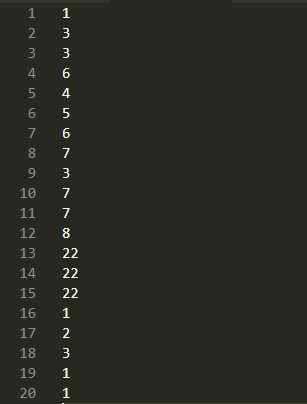
\includegraphics[width=0.27\textwidth,height=\textheight]{media/e1404/image7.jpg}

\end {centerimageenv}

\begin {smalltextenv}

Imagen 2 - \textbf{Fuente:} \emph{Elaboración propia.}

\end {smalltextenv}

\begin {centerimageenv}

\href{https://spaceplace.nasa.gov/galaxy}{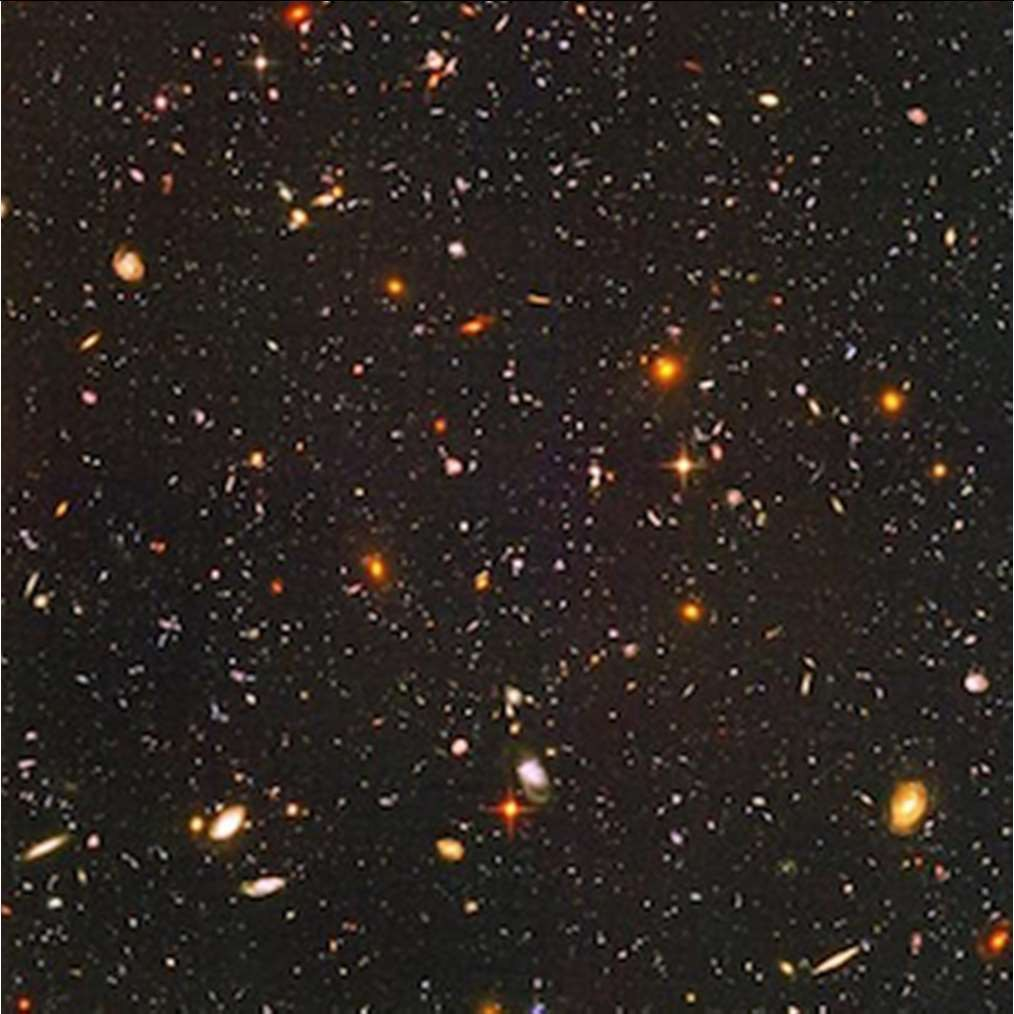
\includegraphics[width=0.45\textwidth,height=\textheight]{media/e1404/image4.jpeg}}

\end {centerimageenv}

\begin {smalltextenv}

Imagen 3 - \textbf{Fuente:} \emph{\href{https://spaceplace.nasa.gov/galaxy}{Nasa}}

\end {smalltextenv}

\begin {centerimageenv}

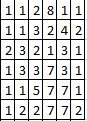
\includegraphics[width=0.25\textwidth,height=\textheight]{media/e1404/image5.jpeg}

\end {centerimageenv}

\begin {smalltextenv}

Imagen 4 - \textbf{Fuente:} \emph{Elaboración propia.}

\end {smalltextenv}

El programa determina el número de cuerpos celestes compara un pixel con los pixeles de sus alrededores para determinar si se trata o no del mismo cuerpo celeste, comenzando de izquierda a derecha y de arriba hacia abajo, es decir empezando con la coordenada (0,0) hasta llegar a la coordenada (n,n) .

El código del programa secuencial, escrito en lenguaje de programación C, se puede encontrar en github \textsuperscript{3}, subido con los permisos pertinentes de los autores. Y este cuenta con el programa secuencial que cuenta los planetas en el archivo de entrada, apoyado con unas librerías desarrolladas por el mismo grupo de investigación que permite obtener el tiempo exacto de ejecución y otra librería que permite conectarse hacia el sistema Tablón \textsuperscript{5} que permitía correr el sistema dentro del clúster de la escuela superior de ingeniería informática.

Para esta prueba, vamos a comparar los tiempos de ejecución en diferentes condiciones obedeciendo las siguientes especificaciones:

\begin {centerimageenv}

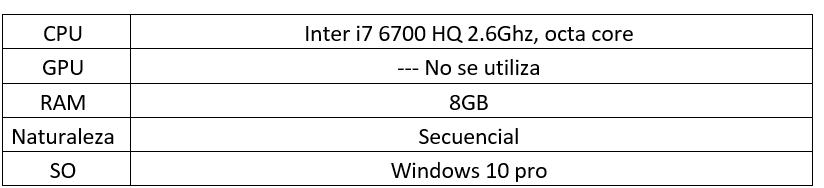
\includegraphics[width=0.45\textwidth,height=\textheight]{media/e1404/resultado1.PNG}

\end {centerimageenv}

\begin {smalltextenv}

Imagen 5 - \textbf{Fuente:} \emph{Especificaciones corrida secuencial de ScanSky - Elaboración propia.}

\end {smalltextenv}

\begin {centerimageenv}

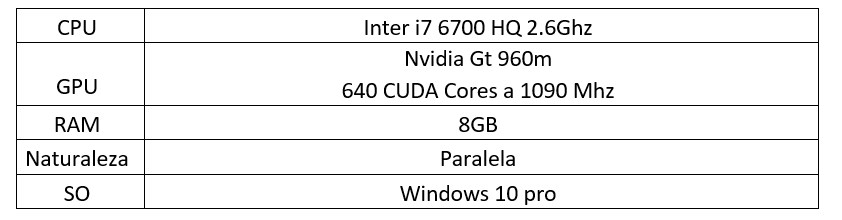
\includegraphics[width=0.45\textwidth,height=\textheight]{media/e1404/resultado2.PNG}

\end {centerimageenv}

\begin {smalltextenv}

Imagen 6 - \textbf{Fuente:} \emph{Especificaciones corrida paralela de ScanSky a través de CUDA - Elaboración propia.}

\end {smalltextenv}

\begin {centerimageenv}

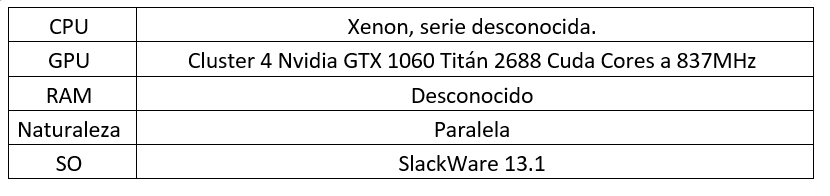
\includegraphics[width=0.45\textwidth,height=\textheight]{media/e1404/resultado3.PNG}

\end {centerimageenv}

\begin {smalltextenv}

Imagen 7 - \textbf{Fuente:} \emph{Especificaciones corrida paralela ScanSky a través de CUDA. Sistema Tablón, UVa - Elaboración propia.}

\end {smalltextenv}

Para estas corridas de prueba se utilizaron 3 tipos de cargas de datos como se indica a continuación:

\begin {centerimageenv}

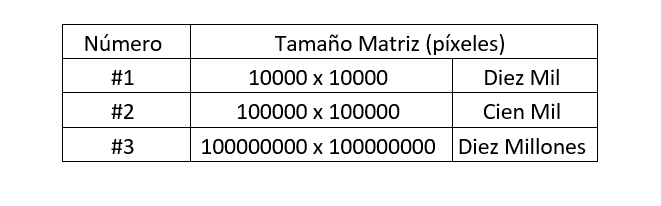
\includegraphics[width=0.45\textwidth,height=\textheight]{media/e1404/resultado4.PNG}

\end {centerimageenv}

\begin {smalltextenv}

Imagen 8 - \textbf{Fuente:} \emph{Set de datos para pruebas con el programa ScanSky - Elaboración propia.}

\end {smalltextenv}

\hypertarget{resultados}{%
\section{Resultados}\label{resultados}}

\begin {centerimageenv}

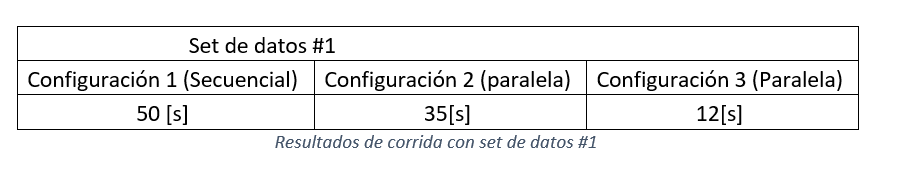
\includegraphics[width=0.45\textwidth,height=\textheight]{media/e1404/resultado5.PNG}

\end {centerimageenv}

\begin {smalltextenv}

Imagen 9 - \textbf{Fuente:} \emph{Elaboración propia.}

\end {smalltextenv}

\begin {centerimageenv}

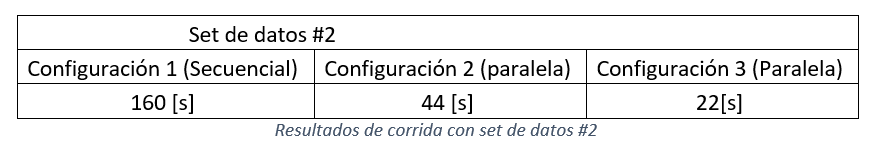
\includegraphics[width=0.45\textwidth,height=\textheight]{media/e1404/resultado6.PNG}

\end {centerimageenv}

\begin {smalltextenv}

Imagen 10 - \textbf{Fuente:} \emph{Elaboración propia.}

\end {smalltextenv}

\begin {centerimageenv}

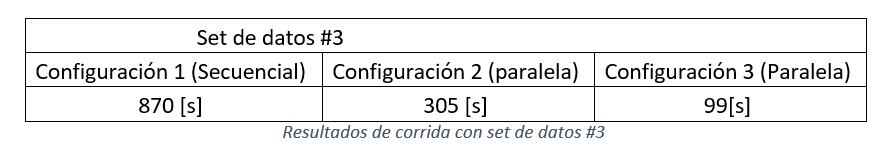
\includegraphics[width=0.45\textwidth,height=\textheight]{media/e1404/resultado7.PNG}

\end {centerimageenv}

\begin {smalltextenv}

Imagen 11 - \textbf{Fuente:} \emph{Elaboración propia.}

\end {smalltextenv}

Como podemos observar en la gráfica anterior, las tres configuraciones tienen una forma similar, pero con una pendiente mucho más pequeña en el caso de la configuración número 3. Y vemos que utilizando la GPU de la computadora de la configuración número 1, obtenemos un resultado que minimiza sobre 3 veces el tiempo utilizado en la aplicación en forma secuencial. Obviamente el código en paralelo utilizando CUDA es mejorable, pero en principio vemos como la computación paralela puede ayudarnos a reducir el tiempo de procesamiento en set de datos pequeños, pero cuando se utilicen set de datos muchos mayores, la diferencia será demasiado grande.

\hypertarget{conclusiones-3}{%
\section{Conclusiones}\label{conclusiones-3}}

\begin{itemize}
\item
  La computación paralela es un tema muy importante en el área de las ciencias de computación y además en muchas industrias como la de la medicina, ingeniería, química, física, aviación, videojuegos entre muchas otras.
\item
  Vemos como en un programa no tan complejo, la programación paralela nos ha ayudado a realizar una aceleración de hasta tres veces menor con un set de datos mediano, pero con set de datos mayores, la aceleración será mucho mayor a comparación de su versión secuencial.
\item
  Es necesario que como escuela de ciencias y sistemas estemos anuentes a estas tendencias tecnológicas que no son recientes pero que tienen mucho auge y demanda en muchas industrias y que podría ser otra ventana de salida para los futuros egresados de nuestra escuela de ciencias y sistemas.
\end{itemize}

\hypertarget{referencias-bibliograficas-3}{%
\section{Referencias bibliográficas:}\label{referencias-bibliograficas-3}}

\begin{itemize}
\item
  \href{https://ecfm.usac.edu.gt/sites/default/files/2017-07/F811-S2017v1_0.pdf}{Programa del curso de física computacional, ECFM, USAC. Disponible en (1)}
\item
  \href{http://www.openmp.org/}{Especificación para computación paralela por medio de paso de mensajes (API). OpenMP (2)})
\item
  \href{https://trasgo.infor.uva.es}{Grupo de investigación, Trasgo. Universidad de Valladolid, España. (3)}
\item
  \href{https://github.com/ErickTejaxun/SkyScan}{Programa ScanSky paralelo y su conversión a su equivalente en versión paralela a través de CUDA. (4)}
\item
  \href{http://www.infor.uva.es/\%7Ejfresno/tablon.php}{Dr.~Javier Fresno, Sistema tablón (5)})
\item
  \href{https://computing.llnl.gov/tutorials/parallel_comp/\#MemoryArch}{Blaise Barney, Lawrence . National Laboratory, ``Introduction to parallel computing'' En línea consultado el 05/04/2019.}
\item
  WOMPAT 2001, International Worskshop on OpenMP Aplication, ``OpenMp Shared Memory Parallel Programing'', Purdue University, School of Electrical and Computer Engineering.
\item
  \href{https://docs.nvidia.com/cuda/}{Nvidia, Cuda Toolkit documentation. En línea Consultado el 01/04/2019.}
\item
  \href{http://web.mit.edu/vex/www/Parallel.pdf}{Michael Skuhersky, MIT. ``Introduction to parallel computing'',En línea consultado el 03/04/2019.}
\end{itemize}

\end {multicols}

\begin {centerimageenv}


\includegraphics[width=0.9\textwidth,height=\textheight]{media/e14publi/09.jpg}

\end {centerimageenv}

\titleformat{\chapter}[display]{\formatchapter}{\labelchapter}{\sepchapter}{\beforecodechapter#1\beforecodechapterparttwo}

\titlespacing*{\chapter} {\leftchapter}{\beforesepchapter}{\afterchapter}

\titleformat{\section}[block]{\formatsection}{\labelsection}{\sepsection}{\beforecodesection#1}

\hypertarget{article05}{%
\chapter{Optimización de sitios web con Google Analytics}\label{article05}}

\begin {multicols}{2}

\BeginKnitrBlock{photobiography3}{media/e1405/image3.jpeg}
\textbf{Anibal Vinicio Gramajo Ramirez}\\
gramajo.anibalv@gmail.com

\medskip

Estudiante de Ingeniería en Ciencias y Sistemas - USAC\\

\medskip

Marketing, SEO, Analytics, análisis, campaña publicitaria.
\EndKnitrBlock{photobiography3}

Una de las principales utilidades de internet es la posibilidad de dar a conocer nuestros productos y servicios a nuevos clientes, a través de diferentes canales de comunicación, tales como redes sociales, foros de debate, motores de búsqueda, entre otros. Debido a la creciente popularidad y extensión de los servicios de telefonía móvil e internet, puede tornarse difícil asegurarse que el mensaje correcto llegue a la persona correcta. Es decir, que nuestros productos y servicios sean vistos por aquellas personas que tengan más probabilidad de adquirirlos o, en otras palabras, segmentar el mercado. Debido a esta necesidad nacen nuevos y diferentes productos que nos ofrecen empresas como Google, estas creadas con el objetivo de sacar el mayor provecho a nuestras campañas publicitarias y así mejorar las ventas de nuestro negocio.

\begin {centerimageenv}

\href{https://medias3.prestastore.com/1264407-pbig/integration-google-adsense-ads.jpg}{
\includegraphics[width=0.35\textwidth,height=\textheight]{media/e1405/image1.jpeg}}

\end {centerimageenv}

\begin {smalltextenv}

Imagen 1 - \textbf{Fuente:} \emph{\href{https://medias3.prestastore.com/1264407-pbig/integration-google-adsense-ads.jpg}{Prestashop.com}}

\end {smalltextenv}

Como estudiantes de Ingeniería en Sistemas, muchas veces ignoramos el alcance que pueden llegar a tener los sistemas que podemos llegar a producir. Sabemos que hoy en día, es prácticamente indispensable para cualquier negocio tener una computadora. Ya sea para llevar control de sus ventas, contactos, recordatorios o simplemente conectarse a internet, se vuelve una necesidad tener un sistema automatizado que permita a las empresas librarse de los viejos libros de papel.

Una de las necesidades que siempre han tenido las empresas es darse a conocer, así como los servicios y productos que ofrecen a posibles nuevos clientes siendo la web el canal más utilizado en esta nueva era. Sin embargo, en el inmenso mundo web es muy difícil lograr que las personas indicadas vean exactamente lo que queremos. Por ejemplo, ¿Cómo logramos que nuestro producto sea visto por determinado grupo de personas? ¿Cómo sabemos cuál anuncio es más eficiente que otro? ¿Cómo sabemos el rango de edades de las personas que nos visitan? Estas y muchas interrogantes más tienen respuesta debido a diversas herramientas que los navegadores y buscadores ponen a nuestra disposición, entre ellas Google.

Siendo estudiante de la carrera de Ingeniería en Sistemas desconocía la estrecha relación que nuestra profesión tendría con otras tan diversas como la contabilidad, publicidad, recursos humanos, etc. Fue hasta que empecé a laborar como freelancer para una empresa estadounidense de marketing que llegué a conocer el impacto que tiene el uso correcto de las campañas publicitarias en línea para la atracción de nuevos clientes a los negocios.

Una de las herramientas que llamó de primero mi atención fue Google Analytics\textsuperscript{1} la cual nos permite conocer más sobre el origen y el comportamiento de los visitantes (posibles clientes) de nuestro sitio web y de esta manera brindarle la información que le interese a fin de captar su atención y hacer, que esa visita se concrete en una venta. Esto es posible gracias a que Google Analytics realiza la inserción de código en los hipervínculos, tanto de nuestro sitio web como de los anuncios de nuestra campaña publicitaria que permite obtener un perfil bastante completo del usuario. Por medio de este código, llamado ``Etiquetas'' (Tags en inglés) podemos obtener características detalladas de nuestros visitantes. Entre las principales se encuentran las siguientes: Edad, ubicación geográfica, idioma, número de páginas de nuestro sitio visitadas, tiempo de duración de la sesión, visitantes de retorno, dispositivo utilizado para la visita, etc.

\begin {centerimageenv}

\href{https://www.simplus.com/wp-content/uploads/2019/06/cpq-1.jpg}{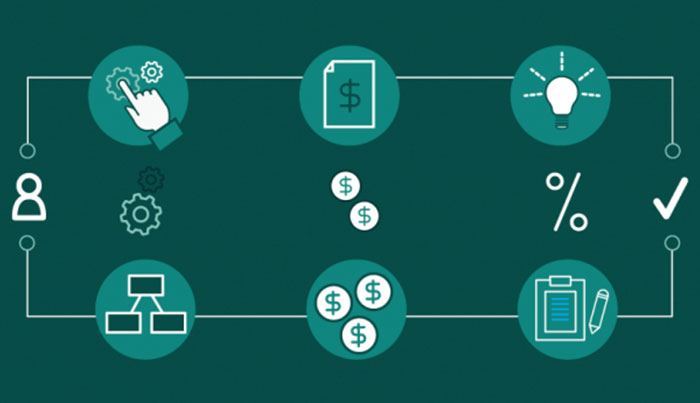
\includegraphics[width=0.35\textwidth,height=\textheight]{media/e1405/image2.jpeg}}

\end {centerimageenv}

\begin {smalltextenv}

Imagen 2 - \textbf{Fuente:} \emph{\href{https://www.simplus.com/wp-content/uploads/2019/06/cpq-1.jpg}{Simplus.com}}

\end {smalltextenv}

Conocer esta información nos ayudará a mejorar la experiencia que el usuario tendrá al visitar nuestro sitio web y podremos ofrecerle contenido específico para su perfil. ¿Estoy atrayendo la audiencia indicada? ¿Están permaneciendo en mi sitio web mis visitantes? Si no, ¿Por qué no? ¿Qué debo cambiar? ¿Les atraen mis ofertas? Como podemos ver, gracias al análisis del usuario que podemos realizar con esta herramienta podemos personalizar nuestro sitio web a fin de satisfacer sus necesidades y aprovechar para hacernos de un nuevo cliente. Podemos, por ejemplo, ofrecer un cupón de descuento a un usuario indeciso que sabemos, ya ha visitado nuestro sitio web con anterioridad sin concretar ninguna compra.

Todo esto se logra por medio de las etiquetas que Google Analytics utiliza. Una de las ventajas de esta herramienta es que posee una poderosa interfaz en línea a la cual podemos acceder desde el sitio web de Google (llamada ``Google Console'') que nos permite configurar las etiquetas que se incrustarán en nuestros enlaces y con ello decidir los aspectos que queremos recopilar de nuestros usuarios. Además, también nos provee de los resultados obtenidos y análisis estadísticos de los visitantes de nuestro sitio. Cabe destacar que el uso de esta herramienta junto con Google Adwords\textsuperscript{2} nos permite crear poderosas campañas publicitarias para una población específica y anuncios que atraigan más visitantes a nuestro sitio web, los cuales obtendrás los mejores productos de acuerdo al perfil que Google Analytics nos permite obtener.

Existe una gran variedad de utilidades que podemos obtener de estas dos herramientas combinadas y con ello, podemos lograr a comprender de una mejor manera a nuestros visitantes, su comportamiento e intereses. Es por ello que Google nos ofrece los programas de capacitación\textsuperscript{3} y certificación en estas herramientas completamente gratis. Esto es una gran ventaja ya que puedes agregar a tu resumen de vida certificaciones\textsuperscript{4} avaladas por una empresa muy reconocida a nivel mundial como lo es Google.

\hypertarget{conclusiones-4}{%
\section{Conclusiones:}\label{conclusiones-4}}

\begin{itemize}
\item
  Al analizar el origen, comportamiento y perfil de los visitantes de nuestro sitio web podemos obtener mejores resultados en nuestras campañas publicitarias al mejorar su experiencia en nuestro sitio y ofrecerle solo productos de su interés.
\item
  El comportamiento de nuestros nuevos visitantes en nuestras páginas de aterrizaje (landing pages) nos permitirá también medir el nivel de efectividad en la manera de promocionar u ofrecer nuestros productos. De esta manera podemos obtener un mayor beneficio de los usuarios que ya se han mostrado interesados.
\item
  Existen diversos medios de capacitarse en herramientas especializadas de diferentes empresas, tales como Google, Yahoo, Microsoft, etc. Muchas de ellas gratuitas que nos permitirán ampliar nuestro conocimiento y agrandar nuestro resumen de vida.
\end{itemize}

\hypertarget{referencias-bibliograficas-4}{%
\section{Referencias bibliográficas:}\label{referencias-bibliograficas-4}}

\begin{itemize}
\item
  \href{https://analytics.google.com/analytics/web/}{Google Analytics (1)}
\item
  \href{https://ads.google.com}{Google Ads (2)}
\item
  \href{https://developers.google.com/training/}{Google Developers (3)}
\item
  \href{https://support.google.com/google-ads/answer/9028754?hl=es-419}{Google Support (4)}
\end{itemize}

\end {multicols}

\titleformat{\chapter}[display]{\formatchapter}{\labelchapter}{\sepchapter}{\beforecodechapter#1\beforecodechapterparttwo}

\titlespacing*{\chapter} {\leftchapter}{\beforesepchapter}{\afterchapter}

\titleformat{\section}[block]{\formatsection}{\labelsection}{\sepsection}{\beforecodesection#1}

\hypertarget{article06}{%
\chapter{El poder de la inteligencia artificial}\label{article06}}

\begin {multicols}{2}

\BeginKnitrBlock{photobiography3}{media/e1406/image1.jpeg}
\textbf{Diego Antonio Momotic Montesdeoca}\\
\href{mailto:diegomomotic@gmail.com}{\nolinkurl{diegomomotic@gmail.com}}

\medskip

Estudiante de Ingeniería en Ciencias y Sistemas - USAC\\

\medskip

Palabras Clave: Inteligencia artificial, redes neuronales, historia, guerra, comparativa, enigma.
\EndKnitrBlock{photobiography3}

Durante el desarrollo de la segunda guerra mundial en los años 1939-1945, fueron llevadas a cabo grandes hazañas de distinta índole, una de estas proezas fue realizada en Bletchley Park Inglaterra, donde la inteligencia británica se encargó de reunir a un grupo de matemáticos, criptógrafos, ajedrecistas y científicos, considerados como los grandes genios de aquella época, con el claro objetivo de descifrar los mensajes codificados de los alemanes, que día a día eran interceptados.

¿Cuál era la dificultad?

Resulta que, los alemanes utilizaban una máquina llamada ``Enigma'' para encriptar sus comunicaciones, este era un dispositivo electrome-
cánico con apariencia similar a una máquina de escribir, como se puede apreciar en la imagen 1.

\begin {centerimageenv}

\href{https://www.neoteo.com/wp-content/uploads/2008/02/enigma2-758x569.jpg}{
\includegraphics[width=0.45\textwidth,height=\textheight]{media/e1406/image3.jpeg}}

\end {centerimageenv}

\begin {smalltextenv}

Imagen 1 - \textbf{Fuente:} \emph{\href{https://www.neoteo.com/wp-content/uploads/2008/02/enigma2-758x569.jpg}{Neoteo.com}}

\end {smalltextenv}

La máquina contaba con ciertas configuraciones que se utilizaban para codificar los mensajes de distinta forma todos los días, es decir, las claves utilizadas para cifrar y descifrar los mensajes cambiaban continuamente, lo que añadía mayor complejidad a la situación. Para que puedas darte una idea la máquina tenía 3.283.883.513.796.974.
198.700.882.069.882.752.878.379.955.261.095.623.
685.444.055.315.226.006.433.616.627.409.666.933.
182.371.154.802.769.920.000.000.000 posibilidades distintas de codificación\textsuperscript{1}.

¿Un número gigantesco no?

A simple vista puede considerarse una tarea prácticamente imposible, sin embargo, te sorpren-
derá saber que, gracias al esfuerzo y genialidad del grupo de personas reunidas en Bletchley Park, liderados por una de las mentes más brillantes de la historia, el matemático, científico y criptógrafo que en la actualidad es considerado uno de los padres de la computación e inteligencia artificial, Alan Turing, el código de la máquina enigma pudo ser descifrado luego de varias modificaciones a finales del año 1942\textsuperscript{2}. Algunos historiadores afirman que el logro sin precedencias de Turing y su equipo de trabajo, acortó la guerra 2 años y salvó aproximadamente 14,000 vidas.

Es una historia impresionante sin duda, pero ¿Qué relación tiene con la Inteligencia Artificial?

Antes de responder a esta pregunta, me gustaría definir los siguientes conceptos:

\begin{itemize}
\item
  \textbf{Inteligencia artificial:} es la simulación de procesos de inteligencia humana por parte de máquinas, especialmente sistemas informáticos. Estos procesos incluyen el aprendizaje, el razonamiento y la autocorrección\textsuperscript{4}.
\item
  \textbf{Redes neuronales:} es un modelo que intenta imitar el funcionamiento del cerebro humano, a través del impulso de entradas y salidas, dejando que la máquina decida el proceso adecuado para transformar las entradas en las salidas solicitadas.
\end{itemize}

Ahora sí, teniendo en mente estos conceptos ¿Considerarías que la inteligencia artificial es capaz de resolver el código enigma?, si tu respuesta es afirmativa ¿Cuánto tiempo crees que tardaría?

Durante el año 2017, según Rafal Janczyk co-fundador de la empresa Enigma Pattern, decidieron replicar el proyecto para descifrar el código de la maquina enigma, pero esta vez utilizarían el poder de la inteligencia artificial para lograrlo. Este proyecto nació, al formularse la pregunta ¿Qué hubiese sido capaz de hacer Alan Turing si hubiese tenido el poder de cómputo actual y el desarrollo que tenemos ahora de la inteligencia artificial? \textsuperscript{5}.

Ahora que conoces la historia y tienes una idea de la complejidad, dificultad y cantidad años de trabajo que conllevó, a las grandes mentes de aquel entonces, el resultado obtenido por el grupo de genios en Bletchley Park es más que sorprendente. Es acá donde radica nuestra verdadera comprensión del poder de procesamiento y capacidad de la inteligencia artificial, ya que con el uso de 2,000 servidores de DigitalOcean (empresa estadounidense que provee servicios en la nube), al trabajar con redes neuronales se logró probar alrededor de 41 millones de contraseñas por segundo y en tan solo 13 minutos la inteligencia artificial fue capaz de descifrar el código. ¿Increíble no?, resulta que aún hay más, el costo real del uso de los 2,000 servidores durante este periodo de tiempo, según DigitalOcean, fue únicamente de 7 dólares\textsuperscript{6}.

Te imaginas el tiempo que se habría acortado la guerra y la cantidad de vidas salvadas, si este tipo de tecnología hubiese existido durante la segunda guerra mundial, sin duda la historia sería muy diferente.

Es muy probable que hoy en día no utilicemos este tipo de herramientas para descifrar códigos en medio de guerras, sin embargo, podemos sacar provecho de ellas en distintas áreas como la robótica, finanzas, educación, entretenimiento, etc. En resumen, no tenemos restricción alguna para su aplicación, más que nuestra imaginación.

\hypertarget{conclusiones-5}{%
\section{Conclusiones:}\label{conclusiones-5}}

\begin{itemize}
\item
  El uso de la Inteligencia artificial es tan útil hoy en día como lo hubiese sido décadas atrás.
\item
  Dotar a los sistemas tecnológicos e informáticos con comportamientos similares a la ``inteligencia humana'', nos ha encaminado, hacia lo que muchos consideran la 4ta revolución industrial.
\item
  Sin darnos cuenta, día con día interactuamos con sistemas que ya se encuentran dotados de inteligencia artificial, como cuando vemos un video en YouTube (que utiliza redes neuronales), o al realizar una compra en el portal de Amazon, entre muchos otros.
\item
  El desarrollo de los proveedores de servicios en la nube como: DigitalOcean, Google Cloud, Azure, Amazon Web Services, etc. Han puesto a nuestro alcance un poder de procesamiento de datos, que hace algunos años atrás no podíamos ni imaginar.
\end{itemize}

\hypertarget{referencias-bibliograficas-5}{%
\section{Referencias bibliográficas:}\label{referencias-bibliograficas-5}}

\begin{itemize}
\item
  \href{https://hipertextual.com/2011/07/la-maquina-enigma-el-sistema-de-cifrado-que-puso-en-jaque-a-europa}{JJ Velasco (12/07/2011) La máquina Enigma, el sistema de cifrado que puso en jaque a Europa.} (27/03/2019) (1)
\item
  \href{https://www.eldiario.es/turing/criptografia/alan-turing-enigma-codigo_0_226078042.html}{Pablo G. Bejerano (06/02/2014). Código Enigma, descifrado: el papel de Turing en la Segunda Guerra Mundial.} (27/03/2019) (2)
\item
  \href{https://culturizando.com/la-historia-del-genio-logro-descifrar-codigo-enigma/}{Mary Villarroel Sneshko (07/06/2018). La historia del genio que logró descifrar el Código Enigma.} (27/03/2019) (3)
\item
  \href{https://searchdatacenter.techtarget.com/es/definicion/Inteligencia-artificial-o-AI}{Margaret Rouse (abril/2017). Inteligencia artificial, o AI.} (27/03/2019) (4)
\item
  \href{https://www.unocero.com/ciencia/descifrando-el-codigo-de-la-maquina-enigma-con-inteligencia-artificial/el-codigo-de-la-maquina-enigma-con-inteligencia-artificial/}{Manuel López Michelone (09/07/2018). Descifrando el código de la máquina Enigma con Inteligencia Artificial} (28/03/2019) (5)(6)
\end{itemize}

\end {multicols}

\begin {centerimageenv}


\includegraphics[width=0.6\textwidth,height=\textheight]{media/e14publi/10.jpg}

\end {centerimageenv}

\titleformat{\chapter}[display]{\formatchapter}{\labelchapter}{\sepchapter}{\beforecodechapter#1\beforecodechapterparttwo}

\titlespacing*{\chapter} {\leftchapter}{\beforesepchapter}{\afterchapter}

\titleformat{\section}[block]{\formatsection}{\labelsection}{\sepsection}{\beforecodesection#1}

\hypertarget{article07}{%
\chapter{Voto Electrónico}\label{article07}}

\begin {multicols}{2}

\BeginKnitrBlock{photobiography3}{media/e1407/sinfoto.jpg}
\textbf{Daniel Orlando Ajuchán Yancis}\\
yancisdl@gmail.com

\medskip

Estudiante de Ingeniería en Ciencias y Sistemas - USAC\\

\medskip

Palabras Clave: Voto electrónico, Sistemas de votación, internet, Voto no presencial.
\EndKnitrBlock{photobiography3}

El voto electrónico es visto como una modalidad en la cual se hace uso de sistemas electrónico-digita-
les en parte o en todo el proceso de votación para acelerar el procesamiento de los resultados, proporcionar asistencia tecnológica y en general, aportar eficiencia en los procesos de elección a cargos populares. Sin embargo, esta definición puede ser demasiado amplia, por lo que es necesario presentar los diferentes sistemas de votación electrónicos conocidos o más implementa-
dos en la actualidad.

\begin {centerimageenv}

\href{https://img-prod-cms-rt-microsoft-com.akamaized.net/cms/api/am/imageFileData/RE2GQ0H?ver=b6da\&q=90\&m=6\&h=540\&w=1900\&b=\%23FFFFFFFF\&l=f\&o=t\&x=184\&y=184\&aim=true}{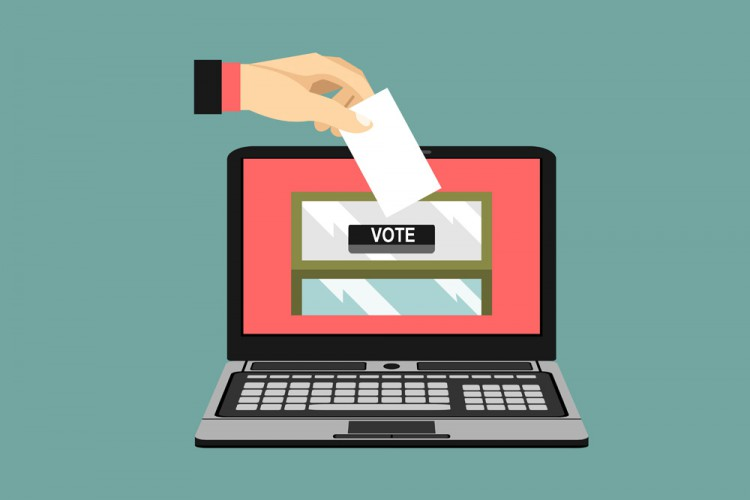
\includegraphics[width=0.45\textwidth,height=\textheight]{media/e1407/image2.jpg}}

\end {centerimageenv}

\begin {smalltextenv}

Imagen 1 - \textbf{Fuente:} \emph{\href{https://img-prod-cms-rt-microsoft-com.akamaized.net/cms/api/am/imageFileData/RE2GQ0H?ver=b6da\&q=90\&m=6\&h=540\&w=1900\&b=\%23FFFFFFFF\&l=f\&o=t\&x=184\&y=184\&aim=true}{Mic}}

\end {smalltextenv}

\hypertarget{registro-electronico-directo-dre-}{%
\section{Registro Electrónico directo --DRE-}\label{registro-electronico-directo-dre-}}

En estos sistemas, los electores emiten su voto utilizando un hardware que puede tener pantalla táctil, botones físicos, etc. Cada uno de estos aparatos cuenta con un disco duro para almacenar el conteo de votos de manera local. Al terminar el evento de votación, los resultados parciales de cada máquina se envían a un servidor para obtener los resultados finales. El problema con este sistema es que no existe una forma de garantizar que el voto emitido se haya registrado de manera correcta, o se haya contabilizado una sola vez debido a que este procedimiento se realiza de forma oculta a los usuarios.

Para evitar el problema del sistema anterior y garantizar que el registro y conteo de votos se realizó de forma correcta, surge la variante que implementa la impresión de una papeleta o \emph{comprobante de auditoría de papel verificado por el votante} -VVPAT-. En esta variante cada uno de los aparatos además de tener la pantalla táctil cuentan con una impresora, que luego de registrar cada voto, imprimen la boleta con la información necesaria que se mostrará al usuario para asegurar que el voto se registró de manera correcta. Algo importante en este sistema es que la boleta impresa no se les entrega a los usuarios, únicamente se muestra (regularmente detrás de un cristal), para luego ser depositada en una urna. Utilizando esta modalidad, se puede llevar un conteo interno en cada aparato o se puede contar únicamente las boletas de cada urna. De esta manera el proceso se hace auditable y se evitan posibles fraudes que pueden darse en sistemas sin VVPAT

\hypertarget{reconocimiento-optico-de-marcasomr-}{%
\section{Reconocimiento Óptico de Marcas--OMR-}\label{reconocimiento-optico-de-marcasomr-}}

En estos sistemas se utilizan papeletas especiales en la que la opción elegida por el votante es reconocida por lectores ópticos. (OMR, OCR, ICR). Hay que notar que esta modalidad en realidad representa una asistencia en el proceso de conteo, ya que únicamente reconocen marcas en las boletas para contabilizarlas.

Existen dos formas de utilizar los lectores de reconocimientos ópticos de marcas, se puede disponer un lector en cada mesa para realizar el conteo cuando el votante introduce su voto en la urna, en este caso se lleva varios conteos parciales. Otra forma es utilizando este método es realizar el conteo de papeletas de forma centralizada pasando todas por un lector de este tipo.

\hypertarget{impresora-de-papeletas-electronicas-ebp-}{%
\section{Impresora de papeletas electrónicas -- EBP-}\label{impresora-de-papeletas-electronicas-ebp-}}

En este sistema, el votante elige su candidato utilizando un aparato muy similar al utilizado en el sistema DRE, y luego de registrar el voto, este aparato imprime una boleta con marcas especiales para que pueda ser leída por un sistema óptico. De esta manera se separa el proceso de emisión de votos y el conteo de los mismos. También genera ayuda a generar confianza, ya que todos los electores pueden verificar su voto en las papeletas antes de depositarlo en las urnas donde serán contabilizados por el sistema óptico. Otro de los beneficios de este sistema es que las boletas serán leídas con un gran porcentaje de confianza, a diferencia de cuando se utilizan boletas marcadas por los usuarios, en donde regularmente los sistemas ópticos no reconocen las marcas de forma correcta. Esta modalidad es considerada una de las seguras, aunque por todo el hardware necesario, también es uno de los métodos más costosos de implementar, no solo en términos monetarios, también es necesario una capacitación adecuada para los usuarios.

Los sistemas descritos anteriormente se caracteri-
zan porque los electores deben emitir su voto de forma presencial, es decir, deben asistir personalmente a los centros de votación autorizados, en donde se realiza manualmente la identificación de cada votante y luego son autorizados a emitir su sufragio, por lo tanto, no hay manera de relacionar el voto con el votante, lo cual se traduce en confianza por parte del elector ya que se mantiene el secreto del voto.

Existe también sistemas no presenciales, en los cuales no se necesita asistir a un lugar en particular, tampoco es necesario hardware especializado como en las modalidades anteriores, en estos casos la autenticación del votante y la emisión del sufragio se realiza en el mismo dispositivo (computadora, tablet, teléfono inteligente), usualmente se realizan a través de internet y siempre son independientes del dispositivo. En estos sistemas, los votos se registran conforme se van emitiendo ya que son transmitidos hacia un servidor, en el cual se tiene un conteo en tiempo real. Si bien este sistema ofrece resultados en tiempo real, también es uno de los más susceptibles a ataques tanto internos (manipulación del software durante su desarrollo) y externos (ataques a los servidores, manipulación de datos durante la transmisión, etc.).

\begin {centerimageenv}

\href{https://img-prod-cms-rt-microsoft-com.akamaized.net/cms/api/am/imageFileData/RE2GQ0H?ver=b6da\&q=90\&m=6\&h=540\&w=1900\&b=\%23FFFFFFFF\&l=f\&o=t\&x=184\&y=184\&aim=true}{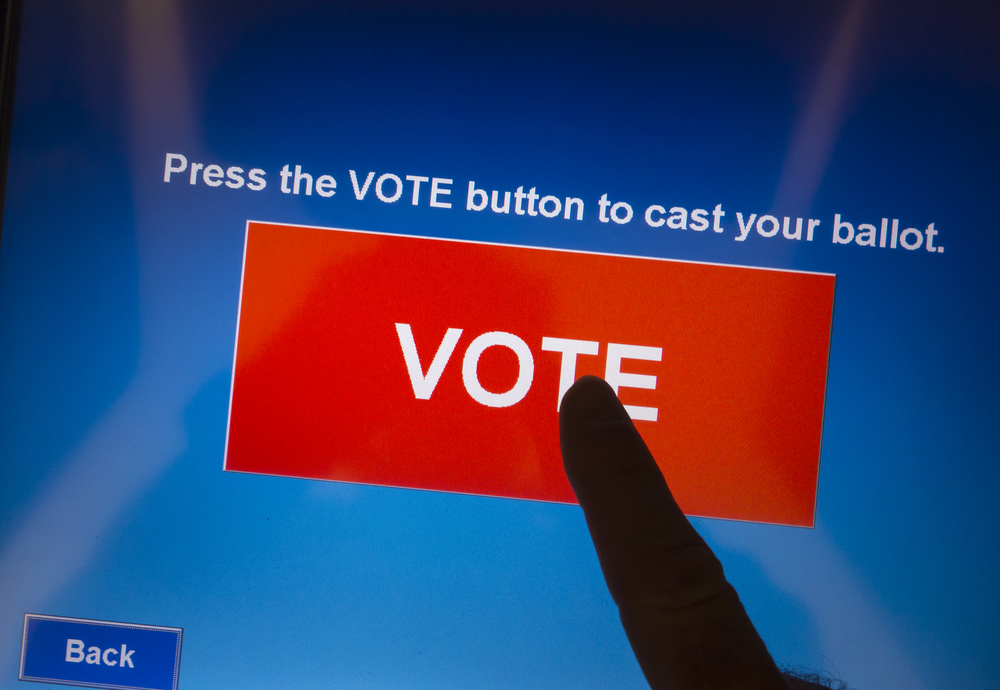
\includegraphics[width=0.45\textwidth,height=\textheight]{media/e1407/image3.jpg}}

\end {centerimageenv}

\begin {smalltextenv}

Imagen 2 - \textbf{Fuente:} \emph{\href{https://img-prod-cms-rt-microsoft-com.akamaized.net/cms/api/am/imageFileData/RE2GQ0H?ver=b6da\&q=90\&m=6\&h=540\&w=1900\&b=\%23FFFFFFFF\&l=f\&o=t\&x=184\&y=184\&aim=true}{Voto electrónico}}

\end {smalltextenv}

Al realizar la autenticación del votante y la emisión del voto en el mismo dispositivo, se corre el riesgo de que se pierda el carácter secreto del voto. Este sistema en particular, presenta muchas debilidades, aunque también ofrece beneficios que no se pueden conseguir con ninguno de los sistemas presenciales, por ejemplo: la accesibilidad ya que no es necesario reunirse en un lugar específico, lo cual beneficia en gran medida a personas con algún impedimento para transportarse de un lugar a otro; también provee rapidez y facilidad de uso ya que la mayoría de personas están familiarizados con dispositivos inteligentes. En general, provee una reducción significativa de costos.

Una de las características más importantes en un sistema de elección a cargos populares, es la transparencia desde antes de iniciar el proceso, hasta el conteo y publicación de los resultados finales, los sistemas de voto por internet y DRE (sin VVPAT) carecen de esta cualidad, en caso de éstos últimos, también presentan el inconveniente de que no todas las personas comprenden el uso de ese tipo de tecnología, esto hace que muchas personas en edad adulta desconfía de estos sistemas y más aún, en áreas rurales en donde el índice de analfabetismo es muy alto.

Independientemente del sistema que se imple-
mente, se debe garantizar que se cumplan las características principales del voto: unicidad, es decir, que cada persona pueda votar una sola vez; el voto debe ser secreto, en otras palabras, que no haya ninguna forma de relacionar al votante con el voto y, por último, que únicamente las personas registradas en el padrón electoral puedan emitir su voto.

\begin {centerimageenv}

\href{https://img-prod-cms-rt-microsoft-com.akamaized.net/cms/api/am/imageFileData/RE2GQ0H?ver=b6da\&q=90\&m=6\&h=540\&w=1900\&b=\%23FFFFFFFF\&l=f\&o=t\&x=184\&y=184\&aim=true}{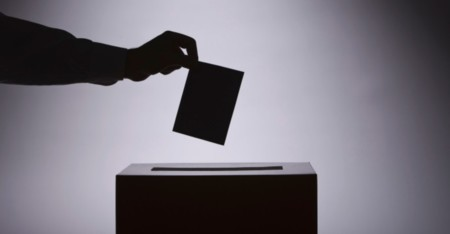
\includegraphics[width=0.45\textwidth,height=\textheight]{media/e1407/image1.jpg}}

\end {centerimageenv}

\begin {smalltextenv}

Imagen 3 - \textbf{Fuente:} \emph{\href{https://img-prod-cms-rt-microsoft-com.akamaized.net/cms/api/am/imageFileData/RE2GQ0H?ver=b6da\&q=90\&m=6\&h=540\&w=1900\&b=\%23FFFFFFFF\&l=f\&o=t\&x=184\&y=184\&aim=true}{Voto electrónico}}

\end {smalltextenv}

\hypertarget{conclusiones-6}{%
\section{Conclusiones:}\label{conclusiones-6}}

\begin{itemize}
\item
  La implementación de sistemas electrónicos y digitales en los procesos de votación ofrecen ventajas frente al sistema tradicional de voto utilizando papeletas impresas, por ejemplo: se obtienen resultados casi instantáneos al finalizar el evento. También proporciona mayor accesibilidad, en cuanto a idiomas, el hardware y software puede ser configurado para mostrar la información en distintos idiomas según sea necesario.
\item
  Los sistemas electrónicos presenciales ofrecen una mayor ventaja en cuanto a prevención de fraudes comparado con los que se hacen por medio de internet.
\end{itemize}

\hypertarget{referencias-bibliograficas-6}{%
\section{Referencias bibliográficas:}\label{referencias-bibliograficas-6}}

\begin{itemize}
\item
  \href{http://www.researchgate.net/publication/259668840_Aspectos_tecnologicos_del_voto_electronico}{Luis Panizo Alonso (12/2017). Aspectos tecnoló-
  gicos del voto electrónico.} (02/04/2019).
\item
  \href{https://www.researchgate.net/publication/267782569_E-Government_El_voto_electronico_sobre_Internet}{Patricia pescado, Ariel Pasini. El voto electrónico sobre internet.} (02/04/2019)
\end{itemize}

\end {multicols}

\begin {centerimageenv}


\includegraphics[width=1\textwidth,height=\textheight]{media/e14publi/04.png}

\end {centerimageenv}

\begin {centerimageenv}


\includegraphics[width=1\textwidth,height=\textheight]{media/e14publi/15.jpg}

\end {centerimageenv}

\titleformat{\chapter}[display]{\formatchapter}{\labelchapter}{\sepchapter}{\beforecodechapter#1\beforecodechapterparttwo}

\titlespacing*{\chapter} {\leftchapter}{\beforesepchapter}{\afterchapter}

\titleformat{\section}[block]{\formatsection}{\labelsection}{\sepsection}{\beforecodesection#1}

\hypertarget{article08}{%
\chapter{El conocimiento no se destruye se transforma}\label{article08}}

\begin {multicols}{2}

\BeginKnitrBlock{photobiography3}{media/e1408/image1.jpeg}
\textbf{Luis Estuardo Azurdia Cárcamo}\\
\href{mailto:luis.azurdia.carcamo@gmail.com}{\nolinkurl{luis.azurdia.carcamo@gmail.com}}

\medskip

Estudiante de Ingeniería en Ciencias y Sistemas - USAC\\

\medskip

Palabras Clave: Educación, Nube, ITIL, Sistemas Operativos, Redes de Computadoras
\EndKnitrBlock{photobiography3}

El mundo de la tecnología siempre está en constante cambio, las personas que trabajan en IT deben estar junto al cambio de la tecnología, al igual que centros educativos que brindan conocimiento a personas que buscan capacitarse como tal. Ninguna persona logrará saberlo todo, pero existe un conocimiento general que es la base de todo lo que se ha construido ahora.

Últimamente el auge de la nube ha solucionado gran cantidad de problemas, dando así la versatilidad de obtener recursos a bajo precio y de forma casi inmediata. Las personas con conocimientos generales, tales como redes, sistemas operativos compiladores entre otros, pueden crear una gran infraestructura por medio de un par de clics con el paso de tiempo resulta más simple poder llevar a la práctica los conocimientos adquiridos en talleres o en alguna clase de programación. La experiencia adquirida al utilizar la nube es grandiosa, solamente es necesario tener el conocimiento de lo que desea hacer, ya que casi todo está enlatado en algún servicio que brinda cada proveedor.

Los proveedores de la nube ofrecen servicios de seguridad externa para la infraestructura tales como un servicio de redes, así como AWS que nos ofrece en el servicio VPC(Virtual private Cloud)\textsuperscript{1}, que a grandes rasgos podemos crear un pequeño data center donde podemos realizar algo muy complejo, cabe resaltar que para entender la utilidad del servicio es necesario aprender el concepto de redes, es posible realizar una traducción del concepto de redes, el cual puede apreciarse en la Figura No.~1 e interpretarla como la Figura No.~2.

La nube especialmente AWS de igual forma sabiendo incluso un poco de ITIL nos ofrecen servicios para poder aplicar dicha metodología, así bien como la gobernanza, el destacado catálogo de servicios\textsuperscript{2}, incluso ofrece de manera intuitiva generar historial

de cambios tales como lo hace el administrador de cambios, como se encuentra en el libro de transición.

El conocimiento general que se adquiere en una educación formal ayuda mucho a comprender en gran medida servicios que nos ofrece la nube. Con el pasar de los años es más sencillo poder comprender el funcionamiento de los servicios y herramientas con tan solo adquirir un ``pincelazo'' de conocimiento.

\hypertarget{conclusiones-7}{%
\section{Conclusiones:}\label{conclusiones-7}}

\begin{itemize}
\item
  Las bases en la educación que se reciben en centros especializados en tecnología tienen todo lo necesario, para ir y descubrir.
\item
  La utilización de nuevas herramientas permite optimizar hasta un 50\% del trabajo realizado, con tan solo tener conocimiento de los conceptos que se desean aplicar.
\item
  Nunca hay perder la emoción de aprender algo nuevo, seguro en algún momento de la vida lo vamos a aplicar
\end{itemize}

\hypertarget{referencias-bibliograficas-7}{%
\section{Referencias bibliográficas:}\label{referencias-bibliograficas-7}}

\begin{itemize}
\item
  \href{https://docs.aws.amazon.com/es_es/vpc/latest/userguide/VPC_Subnets.html}{AWS, documentación VPC} (2019)
\item
  \href{https://docs.aws.amazon.com/es_es/servicecatalog/}{AWS, documentación Service Catalogue}
\end{itemize}

\end {multicols}

\medskip

\begin {centerimageenv}


\includegraphics[width=0.9\textwidth,height=\textheight]{media/e1408/image3.jpeg}

\end {centerimageenv}

\begin {smalltextenv}

Imagen 1 - \textbf{Fuente:} \emph{Elaboración propia.}

\end {smalltextenv}

\medskip

\begin {centerimageenv}

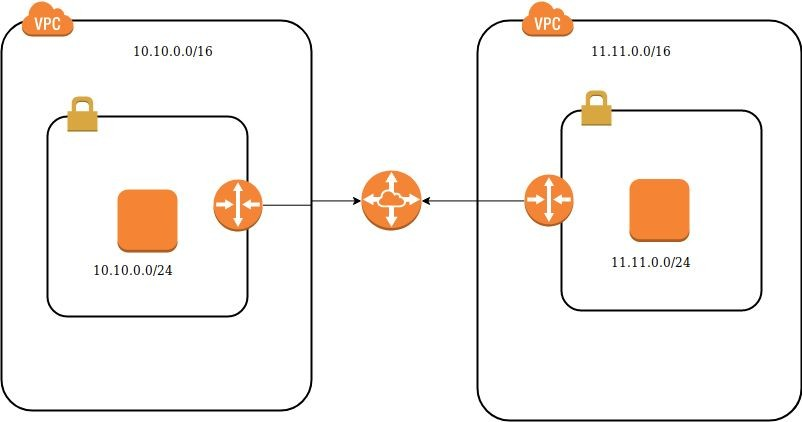
\includegraphics[width=0.9\textwidth,height=\textheight]{media/e1408/image4.jpeg}

\end {centerimageenv}

\begin {smalltextenv}

Imagen 2 - \textbf{Fuente:} \emph{Elaboración propia.}

\end {smalltextenv}

\medskip

\begin {centerimageenv}


\includegraphics[width=1\textwidth,height=\textheight]{media/e14publi/11.jpg}

\end {centerimageenv}

\titleformat{\chapter}[display]{\formatchapter}{\labelchapter}{\sepchapter}{\beforecodechapter#1\beforecodechapterparttwo}

\titlespacing*{\chapter} {\leftchapter}{\beforesepchapter}{\afterchapter}

\titleformat{\section}[block]{\formatsection}{\labelsection}{\sepsection}{\beforecodesection#1}

\hypertarget{article09}{%
\chapter{Moderación de contenido, aplicación práctica de funciones Hash}\label{article09}}

\begin {multicols}{2}

\BeginKnitrBlock{photobiography3}{media/e1409/Imagen.PNG}
\textbf{Carlos Haroldo Mejía Díaz}\\
\href{mailto:Knives50215@gmail.com}{\nolinkurl{Knives50215@gmail.com}}

\medskip

Estudiante de Ingeniería en Ciencias y Sistemas - USAC\\

\medskip

Palabras Clave: Seguridad, Informática, Aplicación práctica, innovación
\EndKnitrBlock{photobiography3}

Las plataformas sociales reciben demasiado contenido a diario, y no es de extrañarse que dentro de tanto contenido se encuentren algunos que no cumplan con los términos y condiciones de estas plataformas. Este contenido aparece de manera pública para que otros la puedan ver. Al tener volúmenes tan masivos, surge la pregunta ¿cómo se controla que el contenido sea legal?

Facebook tiene aproximadamente 147,000 imágenes publicadas cada 60 segundos\textsuperscript{1}. Para la moderación de las imágenes la solución tradicional ha sido la subcontratación.

\begin {centerimageenv}

\href{http://www.pbs.org/independentlens/wp/wp-content/uploads/2018/08/the-cleaners-cubicles-dark-sig-1920x830.jpg}{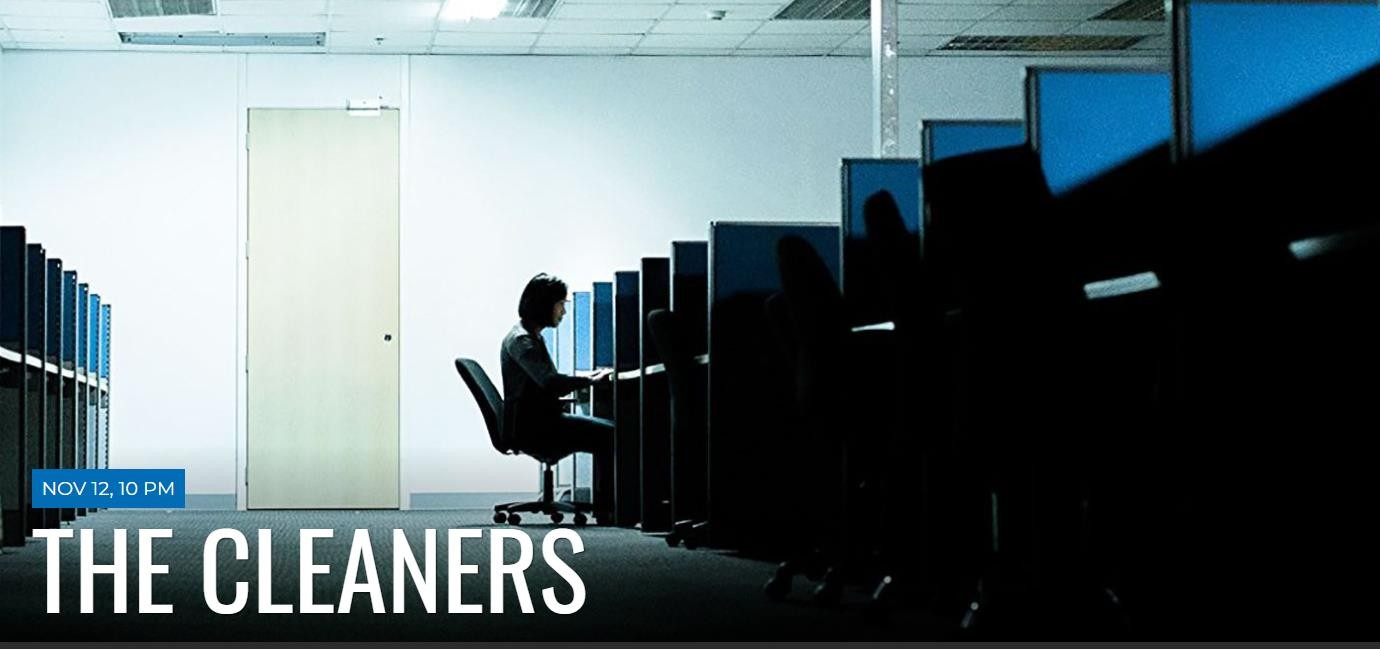
\includegraphics[width=0.45\textwidth,height=\textheight]{media/e1409/image2.jpeg}}

\end {centerimageenv}

\begin {smalltextenv}

Imagen 1 - \textbf{Fuente:} \emph{\href{http://www.pbs.org/independentlens/wp/wp-content/uploads/2018/08/the-cleaners-cubicles-dark-sig-1920x830.jpg}{PBS independant lens}}

\end {smalltextenv}

Existen servicios de monitoreo de imágenes, los cuales mantienen equipos de trabajo que se dedican a filtrar el contenido que ha sido subido a la plataforma en caso de que sea marcado como inapropiado por algún usuario. La mayoría de estos servicios están situados en diferentes partes del mundo, capacitando personal respecto a las políticas de las plataformas que monitorean para que sepan exactamente como clasificar el contenido como inapropiado o legítimo. ``The Cleaners''\textsuperscript{2} es un documental realizado en 2018, el cual muestra el proceso que siguen estas instituciones de moderación de contenido. El documental nos muestra las consecuencias que conlleva la censura de contenido, tanto como para los usuarios como para los moderadores.

El factor humano juega un papel importante en este proceso, la clasificación de imágenes con fines artísticos puede a veces confundirse con contenido explicito, sobrepasando los límites de los términos y condiciones de contenido publicable. El documental hace referencia a este tipo de casos y como es que se resuelven a través del entrenamiento y el criterio de los moderadores.

Una de las desventajas que tiene esta solución es la carga psicológica que tienen esta tarea hacia las personas involucradas. Por Seguridad el personal encargado de la moderación accede a firmar un contrato de confidencialidad. No tienen permitido compartir o discutir con nadie el contenido de lo que han clasificado, incluyendo familiares, amigos o el utilizar servicios psicológicos.

Estas personas revisan contenido que varía desde imágenes ofensivas hasta transmisiones en directo de suicidios o auto mutilación. Cada moderador tiene un sistema de creencias y este contenido impacta en su moralidad. Aunque el contenido sea para ellos moralmente inapropiado, si cumple con las regulaciones, este debe de ser marcado como seguro.

En el documental se comparten diferentes perspectivas sobre el contenido que los moderadores manejan día a día. Algunos ven la posición como un deber en el cual ellos se sacrifican para que los demás no tengan que ver este contenido. Otros han aceptado que es un trabajo como todos los demás. Se comenta también de como la carga es tal que uno de los empleados decidió tomar su propia vida, ya que no pudo soportar el estrés y el impacto del trabajo.

Afortunadamente podemos utilizar nuevas herramientas para reducir el factor humano en estas tareas, pudiendo evitar que más personas estén involucradas en la filtración de contenido. Los desarrollos en inteligencia artificial permiten hacer más fácil la identificación de objetos por medio de entrenamiento de redes neuronales, pudiendo aplicar estas técnicas para la clasificación de contenido ilegal o inapropiado. Dentro de estas herramientas existe PhotoDNA. Esta es una herramienta creada por Microsoft que ha donado a el centro nacional de niños desaparecidos y abuso de menores (National Center for Missing \& Exploited Children). Actualmente esta tecnología es usada por el buscador de Microsoft Bing, su sistema de almacenamiento OneDrive, Gmail, Twitter, Facebook y Adobe Systems.

Microsoft dono esta tecnología hacia el proyecto VIC, el cual es soportado y administrado por el el Centro Nacional para Niños Perdidos y Explotados (NCMEC, por sus siglas en inglés). Esta tecnología usa las funciones hash para identificar de manera única imágenes de la base de datos que el FBI proporciona sobre pornografía infantil, y sobre estos hashes se hace la comparación con el contenido subido a las plataformas. De haber encontrado una coincidencia, se alerta a las autoridades correspondientes para que se tomen las medidas de seguridad establecidas.

Pero, ¿cómo funciona esta tecnología? Primero debemos entender que es una función Hash. Esta son funciones las cuales toman un valor de entrada y lo operan mediante diferentes operaciones matemáticas para obtener un valor específico para la entrada. Estas funciones deben de seguir diferentes propiedades, por ejemplo:

\begin{itemize}
\item
  Estas deben de tomar una entrada y producir un valor el cual siempre será el mismo para el valor de entrada
\item
  Debe de ser lo suficientemente compleja como para evitar llegar al valor de entrada por medio del valor obtenido
\item
  También se debe de evitar colisiones, es decir, si un valor de entrada obtiene un valor con esta función, no debe de existir otra entrada que también obtenga el mismo valor
\end{itemize}

\begin {centerimageenv}

\href{https://img-prod-cms-rt-microsoft-com.akamaized.net/cms/api/am/imageFileData/RE2GQ0H?ver=b6da\&q=90\&m=6\&h=540\&w=1900\&b=\%23FFFFFFFF\&l=f\&o=t\&x=184\&y=184\&aim=true}{
\includegraphics[width=0.45\textwidth,height=\textheight]{media/e1409/image3.jpeg}}

\end {centerimageenv}

\begin {smalltextenv}

Imagen 2 - \textbf{Fuente:} \emph{\href{https://img-prod-cms-rt-microsoft-com.akamaized.net/cms/api/am/imageFileData/RE2GQ0H?ver=b6da\&q=90\&m=6\&h=540\&w=1900\&b=\%23FFFFFFFF\&l=f\&o=t\&x=184\&y=184\&aim=true}{Microsoft, PhotoDNA}}

\end {smalltextenv}

Bajo estas características, se realiza un hash para todas las imágenes de la base de datos. Primero se convierte la imagen a escala de blanco y negro, para evitar que el uso de filtros afecte la detección de estas imágenes. Luego se cambia el tamaño de la imagen y se traza una rejilla para identificar sectores de diferente intensidad de gradientes y también de bordes característicos.

PhotoDNA va un paso más adelante haciendo que los patrones que se identifiquen estén basados en biométrica, permitiendo la generación de códigos únicos para cada imagen respecto a la persona involucrada.

Se aplica a esta imagen una función hash. Esta asegura el evitar las colisiones de 1 en diez billones. En el caso de que el material sean videos, el proceso se ejecuta para cada cuadro del video y se almacena un valor por cada uno.

El tener estas imágenes para generar estos códigos hash es ilegal, por lo que PhotoDNA resolvió esta situación pidiéndole a las agencias de justicia que generen los códigos hash ellos mismos. Estos códigos son distribuidos para los que necesiten utilizarlos por motivos de filtrado de contenido.

Debido al uso de biométrica para la generación de estos códigos, es posible el encontrar coincidencias no solo en las imágenes registradas, sino también en imágenes no registradas. Si se encuentra una coincidencia con alguna de las victimas ya identificadas se pude alertar a las autoridades sobre los posibles autores o distribuidores de este material.

Este método ha sido exitoso para las empresas que lo utilizan. En 2013 esta tecnología ayudo a identificar a un usuario del servicio de almacena-
miento de Verizon\textsuperscript{3}, el cual cargo a su cuenta imágenes de pornografía infantil sin tener en cuenta que parte de los términos y condiciones de este servicio establecen que la plataforma escanea el contenido cargado para encontrar coincidencias de este tipo y alertar a las autoridades.

Verizon no es la única plataforma con este tipo de tecnologías. Dropbox posee también una herramienta para identificar este tipo de anomalías, sin embargo, no ha sido posible identificar que herramienta estén utilizando. En el artículo ``Dropbox Refuses to Explain Its Mysterious Child Porn Detection Software''\textsuperscript{4}, Kate Knibbs trato de hablar con un representante de la compañía para saber más al respecto, sin conseguir una respuesta clara. Ella concluye que la razón es que estén tratando de evitar que los perpetradores utilicen algún tipo de fallo en este sistema para poder seguir cargando contenido ilegal.

Anteriormente se ha establecido que Dropbox utiliza las funciones hash para revisar infracciones de contenido con copyright, utilizando el mismo procedimiento de generación de códigos de identificación únicos para el material registrado\textsuperscript{5}. Este proceso no revisa los materiales personales lo cual lo hace perfecto para respetar la privacidad de los usuarios.

El documental ``The moderators''\textsuperscript{6} trata el mismo tema de monitoreo de contenido, mostrando el proceso de capacitación en el cual los moderadores se someten antes de clasificar contenido. El documental estima que existen aproximadamente más de 150,000 moderadores de contenido, lo cual es el doble del personal en google y casi 9 veces el personal en Facebook. ``No puedes ser dependiente de la automatización'' dice uno de los moderadores encargados de la capacitación de nuevo personal. ``El sistema comete errores. Los humanos son necesarios, de eso estoy seguro.''

``Podemos construir inteligencias artificiales, pero aun necesitas un operador'' Explica otro moderador, ``Definitivamente necesitas a una persona detrás de la maquina''. Con el desarrollo de tecnologías de detección de contenido ilegal, se espera reducir la carga de este tipo de equipos, restringiendo la exposición hacia ciudadanos ajenos a los departamentos de justicia.

\hypertarget{conclusiones-8}{%
\section{Conclusiones:}\label{conclusiones-8}}

\begin{itemize}
\item
  La moderación de contenido es necesaria para las plataformas que almacenan contenido proporcionado por los usuarios.
\item
  El desarrollo de nuevas tecnologías en inteligen-
  cia artificial puede utilizarse para la detección de contenido ilícito.
\item
  Las funciones hash pueden utilizarse más allá de su propósito original de almacenamiento de datos hacia aplicaciones de identificación.
\end{itemize}

\hypertarget{referencias-bibliograficas-8}{%
\section{Referencias bibliográficas:}\label{referencias-bibliograficas-8}}

\begin{itemize}
\item
  \href{https://www.omnicoreagency.com/facebook-statistics/}{Facebook by the numbers. Disponible 10/4/2019 (1)}
\item
  \href{http://www.pbs.org/independentlens/films/the-cleaners/}{The cleaners Disponible 10/4/2019 (2)}
\item
  \href{https://arstechnica.com/information-technology/2013/03/how-verizon-found-a-\%20child-pornographer-in-its-cloud/}{How Verizon found child pornography in its cloud. Disponible 10/4/2019 (3)}
\item
  \href{https://gizmodo.com/dropbox-refuses-to-explain-its-mysterious-child-porn-de-1722573363}{Dropbox Refuses to Explain Its Mysterious Child Porn Detection Software Disponible 10/4/2019 (4)}
\item
  \href{https://gizmodo.com/how-dropbox-knows-when-youre-sharing-copyrighted-files-1555180683}{How Dropbox Knows When You're Sharing Copyrighted Files. Disponible 10/4/2019 (5)}
\item
  \href{https://fieldofvision.org/the-moderators}{The moderators. Disponible 10/4/2019 (6)}
\end{itemize}

\begin {centerimageenv}

\href{https://www.thenewsminute.com/sites/default/files/styles/news_detail/public/moderator_ss.jpg?itok=ND2DBjRA}{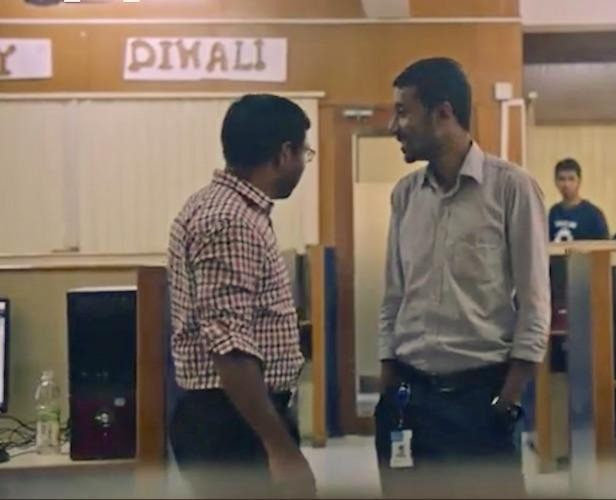
\includegraphics[width=0.5\textwidth,height=\textheight]{media/e1409/image4.jpeg}}

\end {centerimageenv}

\begin {smalltextenv}

Imagen 3 - \textbf{Fuente:} \emph{\href{https://www.thenewsminute.com/sites/default/files/styles/news_detail/public/moderator_ss.jpg?itok=ND2DBjRA}{Screengrab The moderators, Field of vision}}

\end {smalltextenv}

\end {multicols}

\titleformat{\chapter}[display]{\formatchapter}{\labelchapter}{\sepchapter}{\beforecodechapter#1\beforecodechapterparttwo}

\titlespacing*{\chapter} {\leftchapter}{\beforesepchapter}{\afterchapter}

\titleformat{\section}[block]{\formatsection}{\labelsection}{\sepsection}{\beforecodesection#1}

\hypertarget{article10}{%
\chapter{UI/UX - El diseño dentro del software}\label{article10}}

\begin {multicols}{2}

\BeginKnitrBlock{photobiography3}{media/e1410/image1.jpeg}
\textbf{Leonel Eduardo Avila Calvillo}\\
leo.avilac8@gmail.com

\medskip

Estudiante de Ingeniería en Ciencias y Sistemas - USAC\\

\medskip

UI, UX, Usuario, Interfaz, Experiencia, Sistema, Software.
\EndKnitrBlock{photobiography3}

Internet es el hogar de páginas sociales, páginas con recetas, aplicaciones de varios usos, etc. Existen un centenar de páginas web y aplicaciones cuyas funciones pueden llegar a ser idénticas entre sí, pero el modo en que cada una muestra la información o la manera en que el usuario interactúa con ellas es lo que las diferencia. Es por eso que la demanda por una interfaz de usuario efectiva es tan alta.

Pero ¿qué significa \textbf{UI/UX}? y ¿cómo se relaciona con el desarrollo de software? \textbf{UI} son las siglas en ingles de \emph{User Interface}, que significa Interfaz de Usuario, y \textbf{UX} son las siglas en ingles de \emph{User Experience}, que significa Experiencia del Usuario. Estas dos definiciones representan dos prácticas al momento de desarrollar un software. La interfaz de usuario representa todo lo que el usuario ve al momento de iniciar el software, si la primera impresión que este recibe no es favorable, este suele elegir algún otro software con mejor apariencia. Mientras tanto, la experiencia del usuario es como el usuario percibe la funcionalidad del software, su manejabilidad dentro del sistema y como distintas opciones conllevan a otras partes dentro del sistema. Cuando estas dos prácticas son utilizadas juntas, el resultado obtenido es una mayor efectividad en el diseño del software.

\hypertarget{pensamientos-erruxf3neos}{%
\section{Pensamientos erróneos}\label{pensamientos-erruxf3neos}}

Uno de los problemas más comunes al momento de desarrollar un sistema es abocarnos directamente a escribir el código, sin tomar en consideración como el usuario va a utilizar el sistema, dejando la mayor parte de las veces la interfaz de usuario en el olvido, entrando a la línea de pensamiento de "no se verá bien, pero funciona". Si bien el funcionamiento del sistema es importante, no podemos dejar de lado el desarrollo de la interfaz gráfica. Debemos entender que cada parte del sistema, desde el backend hasta el frontend, debe estar bien analizado, sin embargo, debemos tener en cuenta que contar con una interfaz de usuario saturada de elementos, suele convertir la experiencia del usuario a algo desfavorable.

\hypertarget{entendiendo-el-diseuxf1o}{%
\section{Entendiendo el diseño}\label{entendiendo-el-diseuxf1o}}

Al momento de implementar la parte de diseño dentro de nuestro sistema, existen distintos factores que debemos tomar en cuenta. Dentro de estos factores tenemos el enfoque de "el usuario primero", pensando en cómo este utilizará el sistema, y como evitar que este se pierda dentro de la usabilidad del mismo.

\hypertarget{la-relaciuxf3n-entre-ulux}{%
\section{La relación entre Ul/UX}\label{la-relaciuxf3n-entre-ulux}}

Consideremos nuestro sistema como un proyecto de construcción. Un diseñador de UX suele ser el arquitecto, quien es el responsable de la estructura y de los planos del proyecto. Un diseñador de UI vendría siendo el diseñador de interiores de la casa, el que elige los colores, los muebles, el papel tapiz, entre otros.

Estas dos prácticas se deben de trabajar juntas para desarrollar algo que se vea bien y que funcione igual de bien. Si la experiencia del usuario no congenia con el diseño del sistema, al usuario se le hará difícil navegar dentro de esta.

\hypertarget{aspectos-importantes-en-el-diseuxf1o}{%
\section{Aspectos importantes en el diseño}\label{aspectos-importantes-en-el-diseuxf1o}}

Al iniciar la elaboración de una nueva aplicación, muchas veces los desarrolladores se encuentran con distintas problemáticas. Una de las más destacadas es no saber por dónde empezar. Para dar una solución a esta problemática, podemos tomar en consideración distintos aspectos, tales como:

\begin{itemize}
\item
  Tener claro que queremos ofrecer con nuestro sistema, además de entender la problemática que vamos a solventar.
\item
  El diseño debe estar centrado en el usuario. Pensar como actuarían ellos al navegar por las distintas opciones del programa, y como este puede confundirse con la usabilidad del sistema.
\item
  Intenta encontrar que es lo más importante que quieres que haga el usuario. Una vez se haya identificado qué es lo principal, quita las distracciones u otros elementos que no tienen utilidad inmediatamente.
\end{itemize}

\hypertarget{conclusiones-9}{%
\section{Conclusiones:}\label{conclusiones-9}}

\begin{itemize}
\item
  El desarrollo de software no se basa únicamente en programar la funcionalidad, también debemos pensar en cómo el usuario utilizará nuestro sistema, y como ofrecer la mejor experiencia.
\item
  El ofrecer un mejor diseño y una mejor experiencia dentro de nuestro sistema, ayuda a que el usuario final elija nuestra aplicación sobre otras alternativas.
\end{itemize}

\hypertarget{referencias-bibliograficas-9}{%
\section{Referencias bibliográficas:}\label{referencias-bibliograficas-9}}

\begin{itemize}
\item
  \href{https://codigofacilito.com/articulos/design\%20UI\%20y\%20UX}{Luis Enrique Hernández Celaya. Diseño UI y UX.}
\item
  \href{https://www.forbes.com/sites/forbestechcouncil/2019/03/22/our-expectationsof-software-have-changed-its-time-ux-caught-up/\#7cd81793615f}{Claus Jepsen. Our expectations of software have changed - time UX cought up.}
\end{itemize}

\end {multicols}

\medskip
\medskip
\medskip
\medskip
\medskip

\begin {centerimageenv}

\includegraphics[width=1\textwidth,height=\textheight]{media/e14publi/04.png}

\end {centerimageenv}

\medskip
\medskip
\medskip
\medskip

\begin {centerimageenv}

\includegraphics[width=1\textwidth,height=\textheight]{media/e14publi/12.jpg}

\end {centerimageenv}

\titleformat{\chapter}[display]{\formatchapter}{\labelchapter}{\sepchapter}{\beforecodechapter#1\beforecodechapterparttwo}

\titlespacing*{\chapter} {\leftchapter}{\beforesepchapter}{\afterchapter}

\titleformat{\section}[block]{\formatsection}{\labelsection}{\sepsection}{\beforecodesection#1}

\hypertarget{article11}{%
\chapter{Blockchains, un futuro cercano}\label{article11}}

\begin {multicols}{2}

\BeginKnitrBlock{photobiography3}{media/e1411/image1.jpeg}
\textbf{Eder Yafeth Garcia Quiroa}\\
ey16\_619@hotmail.com

\medskip

Estudiante de Ingeniería en Ciencias y Sistemas - USAC\\

\medskip

Palabras Clave: Blockchain, Bitcoins, Japón, Smart Contracts, Startup, Innovación, dApp, Mundo.
\EndKnitrBlock{photobiography3}

Si bien ya se ha escrito mucho sobre Blockchain, ya que es un concepto que lleva más de 40 años de investigación, no es hasta el siglo XXI que se ha desvinculado totalmente del ámbito militar y se ha enfocado más en el cambio de paradigma con importantes consecuencias económicas.

Son muchos los campos de aplicación para la Blockchain, iniciando con la criptografía que dio paso a una larga lista de criptomonedas teniendo a Bitcoin como moneda insignia, pasando por los llamados "Mineros" que tienen el rol de la creación de nuevos bloques y la verificación de los bloques añadidos a la Blockchain y dApp que no son más que app descentralizadas que están desarrolladas como un software que utiliza un token como activo de cambio para la gestión de sus transacciones, hasta llegar más allá del sector de las finanzas , como en el caso de la industria, salud, medios de comunicación e incluso los gobiernos.

Pero ¿Cómo la Blockchain afectara nuestro futuro? Y la respuesta es... ¡ya lo está haciendo! en la actualidad Blockchain ha desarrollado nuevos modelos de negocios y mercados que van desde abrir y cerrar una puerta hasta el seguimiento de los pacientes que abandonen el hospital.

Todo esto debido a que Blockchain se enfoca en acabar con los intermediarios, que hasta el día de hoy se necesitan para realizar operaciones y hacer de estos ecosistemas más rápidos y transparentes.

Un claro ejemplo del poder de la Blockchain en la actualidad son los Smart Contracts, estos son capaces de ejecutarse y hacerse cumplir por sí mismo, de manera autónoma y automática, sin intermediarios ni mediadores. Evitan el lastre de la interpretación al no ser verbal o escrito en los lenguajes que hablamos. Los smart contracts se tratan de "scripts" escritos con lenguajes de programación, siendo los términos del contrato puras sentencias y comandos en el código que lo forma \textsuperscript{2}.

Innovación en estado puro, es como se debería redefinir el concepto de Blockchain ya que ha tenido por consecuencia que una gran cantidad de startups trabajen en desarrollar plataformas o soluciones que utilizan Blockchain. Grandes empresas e incluso gobiernos están sumándose a estas iniciativas, tratando de ser pioneros en su aplicación sobre nuevos usos.

\begin {centerimageenv}

\href{https:}{\includegraphics[width=0.45\textwidth,height=\textheight]{media/e1411/image2.jpeg}}

\end {centerimageenv}

\begin {smalltextenv}

Imagen 1 - \textbf{Fuente:} \emph{\href{https:}{Desconocido}}

\end {smalltextenv}

Un caso reciente de Blockchain en un ámbito diferente al financiero, fue el de Virginia Occidental el primer estado en permitir a sus votantes usar una aplicación, basada en la tecnología Blockchain, este experimento comenzó en marzo y se completó con éxito el 8 de mayo del 2018. La aplicación está estaba destinada, sobre todo, a aquellos militares que están cumpliendo servicio en el extranjero \textsuperscript{3}.

La aplicación fue desarrollada por el startup Voatz, con sede en Boston. Esta permitió a los votantes registrados en 24 países emitir boletas de voto a través de sus teléfonos celulares. Esta fue la solución más segura que consiguieron para facilitar el derecho al voto de los ciudadanos que actualmente hacen vida en el extranjero \textsuperscript{3}.

La aplicación requirió de varios pasos de autenticación antes de que un votante reciba una boleta. Primero, a un usuario elegible se le envía un código de seis dígitos que debe ingresar para desbloquear la aplicación. Después de eso, Voatz requiere que los usuarios carguen una selfie y una identificación con una foto emitida por el gobierno. Las boletas se emiten después de que se verifican las dos imágenes. Una vez que se envían las boletas, los usuarios reciben un correo electrónico que confirma su escogencia. Finalmente, solo después de que se confirmen los votos, se los envía a las oficinas electorales locales en Virginia Occidental. Cabe destacar que, como medida de seguridad, la aplicación no se ejecutará si detecta algún malware en el teléfono \textsuperscript{3}.

A esto hay que sumar que son varios los gobiernos que han estado experimentado con aplicaciones basadas en Blockchain, el caso de Venezuela y su criptomoneda Petro, los gobiernos de China, Rusia, Suiza, Reino Unido, Corea del Sur, Malta, Polonia, Japón, Estados Unidos son algunos de los que ya han activado su interés en las criptomonedas y sobre todo en la tecnología Blockchain. Además, ante el crecimiento de los mercados de Bitcoin en el mundo, también la tecnología Blockchain va ganando terreno, generando nuevas experiencias de organización política como Bitnation o Civic\textsuperscript{4}.

El continente asiático es el más activo en este sentido, y la apuesta de los gobiernos de la región por esta tecnología tiene varios importantes referentes como China, Corea del Sur, Singapur y Japón\textsuperscript{4}.

Este último, Japón, está realizando una gran apuesta de cara a los Juegos Olímpicos de Tokio 2020. Debido a que esta potencia mundial depende enormemente del dinero físico, y casi no practica los pagos electrónicos. Los japoneses tienen una debilidad, les gusta pagar en efectivo, la mayoría de los pagos realizados en el país se basa en billetes y monedas, perdiendo la batalla con sus vecinos asiáticos, China y Corea del Sur, donde el pago electrónico ha ido en aumento y dejándolo muy por detrás de Occidente, donde las tarjetas de crédito y débito son mucho más populares que él efectivo.

Esto significa que el país necesita muchos cajeros automáticos, probablemente tiene más de 200.000, así como cajas registradoras y flotas de vehículos para mover el dinero. Todo esto supone un gasto anual de casi 16,000 millones de euros, la mayoría del cual corre a cargo del sector financiero\textsuperscript{5}.

En agosto del año pasado, el Gobierno anunció planes para ofrecer beneficios fiscales y subsidios a las empresas participantes. Y mientras que todo, desde los pagos con tarjeta de crédito hasta las transacciones con códigos QR, estaría incluido como pago sin efectivo, algunos de los expertos financieros más importantes del país piensan que la mejor forma de que Japón se deshaga del efectivo es mediante la tecnología Bitcoin\textsuperscript{5}.

Mitsubishi UFJ Financial Group (MUFG), el banco más grande del país y el quinto más grande del mundo a nivel de activos, se ha unido a la compañía estadounidense de internet Akamai para construir una red de pagos para el consumidor basada en Blockchain, a tiempo para los Juegos Olímpicos. Si lo logran, podrían generar la red de pagos de consumo más rápida y potente hasta la fecha\textsuperscript{5}.

En este proceso, Japón se convertirá en el proyecto piloto más grande del mundo para probar la Idea de que es posible utilizar un registro criptográfico y una red de ordenadores para crear una forma electrónica de dinero. La prueba incluso podría ayudar al país a recuperar su posición como líder mundial tanto en finanzas como en tecnología, un reinado que no ha tenido durante décadas\textsuperscript{5}.

\hypertarget{conclusiones-10}{%
\section{Conclusiones:}\label{conclusiones-10}}

\begin{itemize}
\item
  Blockchain se basa en la privacidad, esto sumado a una reducción en costo debido a la eliminación de intermediarios en el proceso y al no permitirse su alteración creó una tecnología disruptiva que van a cambiar muchas industrias.
\item
  Esta tecnología aún son solo proyectos en pleno desarrollo, por lo que la revolución aún está lejos de dar todo su potencial, sobre todo cuando los intermediarios, en todos los ámbitos, se han convertido en parte integral de la economía y la sociedad.
\end{itemize}

\hypertarget{referencias-bibliograficas-10}{%
\section{Referencias bibliográficas:}\label{referencias-bibliograficas-10}}

\begin{itemize}
\item
  \href{https://blockchainatberkeley.blog/introducci\%C3\%B3n-a-blockchain-658fdf4e0ff3}{Kunze, F. (2017). Introducción a Block.chain. (1)} (07/04/2019)
\item
  \href{https://academy.bit2me.com/gue-son-los-smart-contracts/}{Academy, B. (2016). Smart contracts. ¿Qué son, cómo funcionan y qué aportan?. (2)} (07/04/2019)
\item
  \href{https://www.coincrispy.com/2018/09/26/virginia-occidental-usara-aplicacion-blockchain-elecciones/}{Romero, R. (2018). Virginia Occidental usará aplicación basada en blockchain en las próximas elecciones. (3)} (08/04/2019)
\item
  \href{https://www.criptonoticias.com/colecciones/gobiernos-mundo-optimizan-procesos-administrativos-tecnoloqia-blockchain/}{Bastardo, J. (2017). Gobiernos del mundo optimizan sus procesos administrativos con tecnología blockchain 1 CriptoNoticias - Bitcoin, blockchains y criptoactivos. (4)} (08/04/2019)
\item
  \href{https://www.technologyreview.es/s/10900/la-\%20apuesta-de-sustitui\%20r-el-efectivo-por\%20-blockchai\%20n-se-decide-en-ja\%20pon}{Milutinovic, A. (2019). La apuesta de sustituir el efectivo por 'blockchain' se decide en Japón. (5)} (08/04/2019)
\end{itemize}

\end {multicols}

\begin {centerimageenv}

\includegraphics[width=0.95\textwidth,height=\textheight]{media/e14publi/13.jpg}

\end {centerimageenv}

\begin {centerimageenv}

\includegraphics[width=0.95\textwidth,height=\textheight]{media/e14publi/14.jpg}

\end {centerimageenv}

\begin {centerimageenv}

\includegraphics[width=0.95\textwidth,height=\textheight]{media/e14publi/15.jpg}

\end {centerimageenv}

\titleformat{\chapter}[display]{\formatchapter}{\labelchapter}{\sepchapter}{\beforecodechapter#1\beforecodechapterparttwo}

\titlespacing*{\chapter} {\leftchapter}{\beforesepchapter}{\afterchapter}

\titleformat{\section}[block]{\formatsection}{\labelsection}{\sepsection}{\beforecodesection#1}

\hypertarget{article12}{%
\chapter{Big Data en el mundo del deporte}\label{article12}}

\begin {multicols}{2}

\BeginKnitrBlock{photobiography3}{media/e1412/image2.jpeg}
\textbf{Rodney Estuardo López Marroquín}\\
\href{mailto:rodx1497@gmail.com}{\nolinkurl{rodx1497@gmail.com}}

\medskip

Estudiante de Ingeniería en Ciencias y Sistemas - USAC\\

\medskip

Palabras Clave: Big data, Tecnología, Deporte, Análisis, Datos.
\EndKnitrBlock{photobiography3}

El análisis de los datos dentro del ámbito deportivo es cada vez más común en cualquier parte del mundo. Gracias a este tipo de observación dado en grandes volúmenes de datos, los cuales, se pueden tratar en diversos eventos deportivos, se facilita la oportunidad de hacer una mejora en la toma de decisiones dentro de este ámbito del deporte, tales como las tácticas que se puedan dar durante un partido, la gestión de fichajes, distancias recorridas, entre otros.

\begin {centerimageenv}

\href{https://www.youtube.com/watch?v=6FP1Da01llc}{\includegraphics[width=0.45\textwidth,height=\textheight]{media/e1412/image4.jpeg}}

\end {centerimageenv}

\begin {smalltextenv}

Imagen 1 - \textbf{Fuente:} \emph{\href{https://www.youtube.com/watch?v=6FP1Da01llc}{YouTube, User: Real Madrid}}

\end {smalltextenv}

Solo durante el desarrollo de algún partido se puede llegar a recolectar hasta 8 millones de datos, algo que a simple vista es casi imposible, ya que el ojo humano puede llegar a retener el 30\% de lo sucedido durante el juego. Gracias a esto, el Big Data permite realizar conclusiones de manera sencilla con base a toda la información recibida previamente.

\hypertarget{quiuxe9n-fue-su-pionero-dentro-de-este-uxe1mbito}{%
\section{¿Quién fue su pionero dentro de este ámbito?}\label{quiuxe9n-fue-su-pionero-dentro-de-este-uxe1mbito}}

El primer deporte en hacer uso del Big Data fue el béisbol, esto gracias a George William James, que, en aquel entonces era un aspirante a articulista deportivo de Kansas. Bill James, como también era conocido, empezó sus análisis a papel junto con su lápiz en los que tomaba en cuenta los registros históricos que tenían los jugadores de béisbol que militaban en las grandes ligas. Todo esto fue realizado a mediados de los años setenta, en donde los artículos de James eran de una forma totalmente distinta a lo que se conocía en esa época, él lo hacía con el fin de tomar en cuenta el juego que realizaba cada deportista en función de los datos estadísticos que se tuvieran disponibles, y no en criterios de una forma más subjetiva. Gracias a dicho trabajo realizado por James, se le considera a este como el padre de la Sabermetría, un análisis empírico general del béisbol.

Mientras los primeros pasos del Big Data en el deporte se dieron de esta manera, en el año 2011 resurge en la ciudad de Hollywood gracias a la película Moneyball, dirigida por Bennet Miller y con Brad Pitt como protagonista, en la cual se recrea el trabajo de Billy Beane en los Oakland Athletics. Dicha película está basada en el libro publicado por Michael Lewis en el año 2003, donde se realiza un análisis de cómo el manager pudo formar un equipo competitivo, esto gracias al uso que les dio a las estadísticas obtenidas de cada uno de sus jugadores de béisbol.

Es así como en deportes como el Hockey, específicamente en la NHL (Liga Nacional de Hockey estadounidense) la cantidad de personas que asisten a cada uno de sus encuentros ha aumentado en un 25\%, todo gracias a que cada uno de ellos puede disfrutar de la gran cantidad de estadísticas que se puede llegar a tener a su alrededor, esto en tiempo real. También es el caso del ciclismo, gracias a Luca, un programa especial de Big Data de la empresa Telefónica, se obtienen diversos tipos de datos, esto a través de unos sensores que pueden llevar incorporados algunos ciclistas, tales como un potenciómetro o una banda de frecuencia cardíaca, lo que permite estudiar su comportamiento en carrera y enviar datos a la nube, para que, posteriormente, puedan ser subidos y se proceda a realizar su análisis de 3 fases. Dentro de estas 3 se ubica de primero la fase descriptiva, luego, le sigue la fase de predicción, y por último la fase de prescripción, lo que permite poder establecer entrenamientos específicos, para así, poder llegar en una buena forma a las fechas en que se disputará alguna actividad o torneo en especial.

Asimismo, se puede visualizar cómo el análisis de los datos supone una revolución, no solamente en el mundo empresarial, también para el deporte profesional y otras áreas en la cual se puede desarrollar fácilmente.

\begin {centerimageenv}

\href{https://www.youtube.com/watch?v=6FP1Da01llc}{\includegraphics[width=0.45\textwidth,height=\textheight]{media/e1412/image6.jpeg}}

\end {centerimageenv}

\begin {smalltextenv}

Imagen 2 - \textbf{Fuente:} \emph{\href{https://www.youtube.com/watch?v=6FP1Da01llc}{YouTube, User: Real Madrid}}

\end {smalltextenv}

\hypertarget{conclusiones-11}{%
\section{Conclusiones:}\label{conclusiones-11}}

\begin{itemize}
\item
  El Big Data es una gran estrategia que permite el análisis de los datos en tiempo real, permitiendo obtener los resultados deseados en un lapso corto de tiempo.
\item
  Actualmente, las diferentes entidades deportivas de algunos equipos están contratando a especialistas en Big Data, todo esto para poder encontrar nuevas ventajas competitivas.
\item
  El análisis de los datos ha evolucionado conforme el tiempo, dejando atrás las técnicas que normalmente eran usadas, dando paso a una nueva era de procedimientos para el análisis y el manejo correcto, además de eficiente, de los datos.
\end{itemize}

\hypertarget{referencias-bibliograficas-11}{%
\section{Referencias bibliográficas:}\label{referencias-bibliograficas-11}}

\begin{itemize}
\item
  \href{https://www.youtube.com/watch?v=6FP1Da01llc}{Real Madrid C.F. (15/03/2019). Behind Real Madrid \textbar{} Player performance.} (22/03/2019).
\item
  \href{http://sportsmadeinusa.com/beisbol/mlb/bill-james-el-padre-del-sabermetrics-moderno/}{Ángel Carrillo. (28/11/2014). Bill James, el ``padre'' del Sabermetrics moderno.} (25/03/2019).
\item
  \href{https://phys.org/news/2018-12-big-impacting-sports-analytics.html}{Mary Ann Liebert. (20/12/2018). How is big data impacting sports analytics?} (26/03/2019).
\item
  \href{https://dataconomy.com/2018/01/big-data-revolutionizing-favorite-sports-teams/}{Ryan Ayers. How big data is revolutionizing sports.} (27/03/2019).
\end{itemize}

\medskip
\medskip

\begin {centerimageenv}

\href{https://www.youtube.com/watch?v=6FP1Da01llc}{\includegraphics[width=0.45\textwidth,height=\textheight]{media/e1412/image5.jpeg}}

\end {centerimageenv}

\begin {smalltextenv}

Imagen 3 - \textbf{Fuente:} \emph{\href{https://www.youtube.com/watch?v=6FP1Da01llc}{YouTube, User: Real Madrid}}

\end {smalltextenv}

\end {multicols}

\medskip
\medskip

\begin {centerimageenv}

\includegraphics[width=1\textwidth,height=\textheight]{media/e14publi/16.jpg}

\end {centerimageenv}

\titleformat{\chapter}[display]{\formatchapter}{\labelchapter}{\sepchapter}{\beforecodechapter#1\beforecodechapterparttwo}

\titlespacing*{\chapter} {\leftchapter}{\beforesepchapter}{\afterchapter}

\titleformat{\section}[block]{\formatsection}{\labelsection}{\sepsection}{\beforecodesection#1}

\hypertarget{article13}{%
\chapter{Desafíos y oportunidades del Cloud Computing en Guatemala}\label{article13}}

\begin {multicols}{2}

\BeginKnitrBlock{photobiography3}{media/e1413/image1.jpeg}
\textbf{Julia Argentina Sierra Herrera}\\
julyargesh@gmail.con

\medskip

Estudiante de Ingeniería en Ciencias y Sistemas - USAC\\

\medskip

Palabras Clave: Paas, Saas, Iaas, Informacion, Seguridad, Costos
\EndKnitrBlock{photobiography3}

Los servicios en la nube que se pueden encontrar son diversos, estos han realizado varios cambios en las empresas, la mayoría de estos positivos, permitiendo realizar tareas de manera sencilla.

\hypertarget{por-quuxe9-deberuxedamos-de-utilizar-cloud-computing}{%
\section{¿Por qué deberíamos de utilizar Cloud Computing?}\label{por-quuxe9-deberuxedamos-de-utilizar-cloud-computing}}

El Cloud Computing, nos ofrece grandes oportuni-
dades porque es lo que se está utilizando, además en la carrera de Ingeniería en Ciencias y Sistemas, la innovación es algo esencial porque el cambio es constante.

En los últimos años América Latina ha hecho una importante apuesta por el desarrollo de las Tecnologías de la Información, situándose en una posición de liderazgo. De hecho, será la zona con el crecimiento más rápido del planeta, con un ritmo 1,74 veces superior que la media mundial, según publica Altag, que calcula que la tendencia de incremento de la industria TI será del 10,3\% en 2013\textsuperscript{1}.

En la imagen 1 se muestra como Guatemala no preparada para estos cambios, en esta misma grafica se muestran los demás países de Latinoamé-
rica, a pesar que Guatemala no está situada en la última posición, podemos ver que ninguno de los países de Latinoamérica está preparado, lo que genera pérdidas, para empresas internacionales o diferentes trabajos donde se requiera el conocimiento de estas nuevas tecnologías, lo que nos permite visualizar que como estudiantes de ingeniería en sistemas es un compromiso, lograr que las gráficas cambien y nuestra preparación en estas nuevas tecnologías logren un avance no solo en una estadística si no que beneficien el desarrollo de nuestro país.

\begin {centerimageenv}

\href{https://evaluandocloud.com/cloud-computing-en-america-latina/}{\includegraphics[width=0.45\textwidth,height=\textheight]{media/e1413/image2.png}}

\end {centerimageenv}

\begin {smalltextenv}

Imagen 1 - \textbf{Fuente:} \emph{\href{https://evaluandocloud.com/cloud-computing-en-america-latina/}{Cloud computing in Latin America Current situation and policy proposals, Economic Commission for Latin America and the Caribbean ECLAC.}}

\end {smalltextenv}

La revolución digital está trayendo consigo unas necesidades excepcionales de cómputo y almacenamiento. Muchas empresas tuvieron que crear sus propios centros de datos. Sin embargo, su coste es altísimo. La evolución definitiva vino de la mano del modelo Cloud Computing y la ideación y creación de un sistema completo (sostenible y de extremo a extremo) de prestación de servicios TI \textsuperscript{2}.

\hypertarget{de-quuxe9-manera-utilizamos-cloud-computing}{%
\section{¿De qué manera utilizamos Cloud Computing?}\label{de-quuxe9-manera-utilizamos-cloud-computing}}

Las empresas comúnmente adquieren el Software como Servicio (SaaS, por sus siglas en inglés) porque carecen de recursos para instalar el software, y porque se paga por uso. El utilizar SaaS nos permite que los involucrados del proyecto, tengan acceso a la información desde cualquier dispositivo con el que puedan estar conectados a internet. Esto también proporciona una seguridad de datos, porque cuando se tengan fallos en algún dispositivo, la integridad de los datos no será dañada.

Los servicios del Cloud Computing nos traen diferentes oportunidades, pero el servicio que más ha conseguido un impacto en las empresas ha sido laaS, porque al iniciar una empresa se reducen costos iniciales, permitiendo que sin poseer un espacio físico se tengan los recursos necesarios, obteniendo servicios por consumo, también permite cambios sobre lo que utilizamos, sin generar mayores gastos que se dan en sistemas físicos, lo que permite no tener que realizar cambios en información que generan pérdidas de tiempo y aumento de gastos.

Plataforma como servicio, es utilizado por empresas orientadas a desarrollo de software, este servicio provee lo mismo que laaS con la diferencia que no se debe de preocupar por el mantenimiento. Las empresas eligen utilizar este servicio debido a que tienen herramientas de desarrollo y herramientas empresariales, que proporcionan reducción de tiempos en la programación.

\hypertarget{quuxe9-oportunidades-genera-el-cloud-computing}{%
\section{¿Qué oportunidades genera el Cloud Computing?}\label{quuxe9-oportunidades-genera-el-cloud-computing}}

El Cloud Computing permite que los usuarios se beneficien reduciendo costos y tiempos, que son parte esencial en una empresa al momento de intentar lograr los conceptos de gerencia eficiencia y eficacia, se trata de utilizar la menor cantidad de recursos físicos, se ofrece optimizar recursos, cobros por tiempo de utilización, se evitan pérdidas de tiempo y se logra a la vez evitar contactos con distribuidores, técnicos, entre otros que generan gastos para la empresa.

Logra que sea conveniente en la forma en que se adquieren servicios, la facilidad con que se realizan aplicaciones, e ingreso de datos, permite cambios de acuerdo a los requerimientos sin generar costos adicionales. Es fácil detectar en que se están realizando los gastos y permite visualizar de mejor manera como los cambios generados benefician o afectan las empresas.

\hypertarget{quuxe9-desafuxedos-nos-genera-utilizar-cloud-computing}{%
\section{¿Qué desafíos nos genera utilizar Cloud Computing?}\label{quuxe9-desafuxedos-nos-genera-utilizar-cloud-computing}}

Al involucrarnos con la utilización del Cloud Computing, el idioma es uno de los desafíos debido a que la documentación y comunicación con los proveedores debe de ser en el idioma inglés.

Los distribuidores de los servicios no se hacen cargo de las perdidas o robo de datos. Entonces el desafío como ingeniero en sistemas es identificar de qué manera se debería de realizar la estructura para utilizar Cloud Computing, conocer que datos están seguros dentro y fuera de los servicios que se están contratando.

En la Imagen 2 se muestra que el 95\% de los encuestados en Latinoamérica ven positivo el uso del Cloud Computing, además presenta que el 32\% de los encuestados piensa que el inhibidor para su adopción es la seguridad. Por lo tanto, podemos determinar que la seguridad nos da un parámetro para decidir por que utilizar o no el Cloud Computing.

\begin {centerimageenv}

\href{https://www.comunidadbaratz.com/blog/la-adopcion-e-impacto-del-cloud-computing-en-el-mundo/}{\includegraphics[width=0.45\textwidth,height=\textheight]{media/e1413/image3.png}}

\end {centerimageenv}

\begin {smalltextenv}

Imagen 2 - \textbf{Fuente:} \emph{\href{https://www.comunidadbaratz.com/blog/la-adopcion-e-impacto-del-cloud-computing-en-el-mundo/}{Comunidad BTZ}}

\end {smalltextenv}

Utilizar Cloud Computing genera nuevos desafíos para un programador, ingeniero en ciencias y sistema o cualquier otro cargo relacionado con tecnología, porque comprender de qué manera funcionan estos servicios genera el conocimiento de tecnologías que permiten que la utilización del Cloud Computing sea eficaz.

\hypertarget{conclusiones-12}{%
\section{Conclusiones:}\label{conclusiones-12}}

\begin{itemize}
\item
  El desafío mas importante es mantenerse actualizado sobre la nueva tecnología que se está desarrollando.
\item
  El Cloud Computing nos permite tener una empresa eficiente y eficaz.
\item
  El desarrollo en el país también depende de una educación y compromiso con las nuevas tecnologías para poder ser desarrolladas.
\item
  El Cloud Computing debe ser utilizado de la forma correcta para lograr que no se exponga la información importante.
\end{itemize}

\hypertarget{referencias-bibliograficas-12}{%
\section{Referencias bibliográficas:}\label{referencias-bibliograficas-12}}

\begin{itemize}
\item
  \href{https://blog.apser.es/2016/12/16/cloud-computing-environment-principales-desafios}{Asper (16/12/2016). Los principales desafíos del cloud computing enviroment. (1)}
\item
  \href{https://www.comunidadbaratz.com/blog/la-adopcion-e-impacto-del-cloud-computing-en-el-mundo/}{Comunidad Baratz (17/11/2013) La adopción e impacto del cloud computing en el mundo. (2)}
\item
  \href{https://evaluandocloud.com/cloud-computing-en-america-latina/}{Evaluando Cloud (7/06/2015) Cloud Computing en America Latina (3)}
\item
  \href{https://recursos.evaluandosoftware.com/opinion/predicciones-la-nube-2018/?sf_action=get_results\&_sft_modalidad=cloud}{Evaluando Software (2017) Predicciones para la nube 2018. (4)}
\item
  \href{http://www.emb.cl/gerencia/articulo.mvc?xid=519\&sec=12}{Hernán Calderale. Desafios y oportunidades para los CIOs en la era de la nube. (5)}
\end{itemize}

\end {multicols}
\medskip

\begin {centerimageenv}

\includegraphics[width=1\textwidth,height=\textheight]{media/e14publi/17.jpg}

\end {centerimageenv}

\begin {centerimageenv}

\includegraphics[width=1\textwidth,height=\textheight]{media/e14publi/18.jpg}

\end {centerimageenv}

\medskip

\begin {centerimageenv}

\includegraphics[width=1\textwidth,height=\textheight]{media/e14publi/19.jpg}

\end {centerimageenv}

\titleformat{\chapter}[display]{\formatchapter}{\labelchapter}{\sepchapter}{\beforecodechapter#1\beforecodechapterparttwo}

\titlespacing*{\chapter} {\leftchapter}{\beforesepchapter}{\afterchapter}

\titleformat{\section}[block]{\formatsection}{\labelsection}{\sepsection}{\beforecodesection#1}

\hypertarget{article14}{%
\chapter{Es hora de regular el contenido de internet}\label{article14}}

\begin {multicols}{2}

\BeginKnitrBlock{photobiography3}{media/e1414/image1.jpeg}
\textbf{Rubén Emilio Osorio Sotorro}\\
\href{mailto:rubenosorio88@gmail.com}{\nolinkurl{rubenosorio88@gmail.com}}

\medskip

Estudiante de Ingeniería en Ciencias y Sistemas - USAC\\

\medskip

Palabras Clave: Internet, tecnología, información, redes sociales, conocimiento, ciencia, regularización.
\EndKnitrBlock{photobiography3}

Si bien el internet es una herramienta muy poderosa y necesaria en pleno siglo XXI, con millones y millones de páginas en las cuales podemos consultar el clima, que ofertas tendrá nuestro restaurante favorito, poder reservar un vuelo a la Patagonia simplemente con un par de clics en la comodidad de nuestro hogar, solo imaginemos un momento si en realidad todas las personas que tenemos acceso a internet lo usáramos para nutrir nuestros conocimientos, para hacer investigaciones y compartir resultados donde más personas se unan y se genere más conocimientos a partir de un trabajo colectivo como se observa en la imagen 1, pero claro, eso no significa que no se haga, la página del MIT publica muchos artículos que son base para muchas otras personas que pueden empezar una investigación o continuarla basándose en estos artículos, pero si hacemos una media de para que usamos más el internet en este siglo veremos que lo menos que se hace es investigar, muchos se enfocan más en el uso de redes sociales, intentando ser famosos de alguna forma, por ejemplo, al subir algo que muchos llamarían ``gracioso'' a páginas como Instagram, todo esto es el comienzo de una plaga llamada ``influencers''. Como se observa en la imagen 1 un grupo de personas que únicamente se encargan de subir contenido (la mayoría basura en mi criterio) a Internet, y además hay marcas que por hacerles publicidad les pagan por ello al tener una gran cantidad de personas que las siguen y admiran, y ese en realidad es el problema, porque estas personas no son unos genios de la matemática, ni hablan sobre el cosmos, muchos se dedican a hacer retos verdaderamente tontos que no tienen algún sentido, como meterse un preservativo por la nariz y sacarlo por la boca como en la imagen 2, muchos repudian este tipo de contenido inútil, pero hay otros que si les llama la atención, y como ven que la persona famosa del internet lo hace, ellos también deben hacerlo.

\begin {centerimageenv}

\href{https://www.shutterstock.com/image-photo/cloud-computing-future-technology-people-concept-728826436}{\includegraphics[width=0.35\textwidth,height=\textheight]{media/e1414/image3.jpeg}}

\end {centerimageenv}

\begin {smalltextenv}

Imagen 1 - \textbf{Fuente:} \emph{\href{https://www.shutterstock.com/image-photo/cloud-computing-future-technology-people-concept-728826436}{Syda Productions}}

\end {smalltextenv}

Leyendo un artículo del famoso noticiero británico BBC que tiene como título ``\emph{El 90\% de lo que está en internet es basura}'', en dicho escrito podemos encontrar que ellos describen un par de leyes de personas que se dedicaron a analizar las siguientes situaciones:

Ley de Pommer, una persona puede cambiar de opinión en base a la información que lee en internet. La naturaleza de ese cambio será que pasará de no tener ninguna opinión a tener la opinión errada.

Y es que esta ley tiene tanta razón con que hay personas creen todo lo que dice internet, y si hablamos de que la mayoría de contenido es basura, entonces la información también es basura.

\begin {centerimageenv}

\href{https://bellezaslatinas.com/salud-del-adolescente/peligrosos-retos-virales-entre-adolescentes}{\includegraphics[width=0.35\textwidth,height=\textheight]{media/e1414/image5.jpeg}}

\end {centerimageenv}

\begin {smalltextenv}

Imagen 2 - \textbf{Fuente:} \emph{\href{https://bellezaslatinas.com/salud-del-adolescente/peligrosos-retos-virales-entre-adolescentes}{Patricia Carambula}}

\end {smalltextenv}

Es donde comienzo a hablar sobre las restricciones que debe tener internet y es que si algo no está regulado se pierde el control, el problema a veces es ¿Quién lo regula? ¿Cómo decide que es bueno o malo?, pero es que es una realidad, la NASA podría hacer una transmisión desde marte que no muchas personas mirarían, pero uno de los videos más vistos en la plataforma de videos Youtube es un tipo cantando sobre una manzana, una piña, y un lápiz, visto por más de 255 millones de personas hasta este año 2019.

\begin {centerimageenv}

\href{ttps://www.youtube.com/results?search_query=pen+apple+pineapple+pen}{\includegraphics[width=0.45\textwidth,height=\textheight]{media/e1414/image6.jpeg}}

\end {centerimageenv}

\begin {smalltextenv}

Imagen 3 - \textbf{Fuente:} \emph{\href{ttps://www.youtube.com/results?search_query=pen+apple+pineapple+pen}{Youtube usuario: Pikotaro}}

\end {smalltextenv}

Está bien, páginas como Youtube no nos obligan a ver este tipo de contenido, el problema quizá es que este tipo de páginas alientan a las personas a seguir compartiendo este contenido ya que reciben un pago enorme por la cantidad de visitas que llegan a tener sus videos, pero sí utilizan algoritmos para hacer recomendaciones como ``lo más visto'' o los temas ``hot'' del momento, ``El sistema de recomendación de vídeos de YouTube se enfrenta, una vez más, a la polémica. Algunos usuarios han criticado el algoritmo de la plataforma, alegando que promueve los vídeos de teorías de la conspiración y de \emph{fake news}.''\textsuperscript{2}

Y es que como todo en la vida el dinero es motivación, si no me van a pagar por hacer tonterías en internet, para que las voy a hacer, hace poco Mark Zuckerberg (creador de la famosa red social Facebook) hablaba de ``Regular el internet'' como se menciona en CNN ``El fundador de Facebook, \href{https://cnnespanol.cnn.com/tag/mark-zuckerberg/}{{Mark Zuckerberg,}} publicó una misiva haciendo un pedido a los gobiernos y los reguladores para que impongan más controles sobre lo que se publica en internet, la protección de datos y otro temas''.\textsuperscript{3}

Zuckergerg propone 4 aspectos que requieren especial cuidado:

\begin{enumerate}
\def\labelenumi{\arabic{enumi}.}
\item
  Sobre el contenido perjudicial: Mark menciona que se debe estandarizar y hacer más rígidas las políticas sobre el contenido que se sube a cada plataforma y en sus procesos, se necesita un enfoque más estandarizado.
\item
  Integridad en las elecciones: También menciona que deben haber leyes que se aplican en cada gobierno que debe regular que clase de contenido es permitido por cada candidato a hacerse publicidad, también de esto viene el tema de los ``netcenters'' y encuestas falsas donde posicionan a un candidato a favor sobre los otros.
\item
  Privacidad de los datos: si bien todo lo que está e internet pareciera no ser privado para nada, ``La nueva regulación de privacidad en los Estados Unidos y en todo el mundo debería basarse en las protecciones que proporciona el Reglamento General de Protección de Datos (GDPR, por sus siglas en inglés). Éste debería proteger tu derecho a elegir cómo se usa tu información y no de requerir que los datos se almacenen de manera local, ya que lo haría más vulnerable al acceso injustificado.''\textsuperscript{4}
\item
  Portabilidad en los datos: aquí se refiere que hay que aclarar las reglas sobre quien es responsable de proteger la información que las personas cuando esta se mueve entre cada servicio.
\item
  En mi punto de vista personal, contenido que no promueve nada bueno en las personas es perjudicial, perjudicial para sus mentes.
\end{enumerate}

\hypertarget{conclusiones-13}{%
\section{Conclusiones:}\label{conclusiones-13}}

\begin{itemize}
\item
  Se debe dar menos prioridad a videos y contenidos de influencers en las redes pagándoles poco sobre su contenido.
\item
  La regulación es un tema que se da abasto y se deben tener muchos debates al respecto.
\item
  El contenido que cada persona consume en internet es siempre su responsabilidad, pero las plataformas deben de promover contenido más informativo, ya depende del usuario si lo ve o no.
\end{itemize}

\hypertarget{referencias-bibliograficas-13}{%
\section{Referencias bibliográficas:}\label{referencias-bibliograficas-13}}

\begin{itemize}
\item
  \href{https://www.bbc.com/mundo/noticias/2014/01/140122_internet_leyes_reglas_finde}{BBC Mundo (26/01/2014) El 90\% de lo que está en internet es basura.}
\item
  \href{https://as.com/meristation/2018/02/12/noticias/1518448140_173090.html}{Xose Llosa (12/2/2018). Youtube dejará de visibilizar a creadores tóxicos}
\item
  \href{https://cnnespanol.cnn.com/video/sugerencia-facebook-regulacion-internet-mark-\%20zuckerberg-pedido-gobiernos-controles-internet-proteccion-datos-serbia-dinero/}{Xavier Serbia (01/04/2019). ¿Qué sugiere Facebook para regular internet?}
\item
  \href{https://www.fortuneenespanol.com/tecnologia/regular-internet-zuckerberg/}{Sandra Pérez (02/04/2019). 4 Formas de regular internet según Zuckerberg.}
\end{itemize}

\end {multicols}

\begin {centerimageenv}

\includegraphics[width=1\textwidth,height=\textheight]{media/e14publi/02.png}

\end {centerimageenv}

%%%%%%%%%%%%%%%%%%%%%%%%%%%%%%%%%%%%%%%%%%%%%%%INIT BACKCOVER%%%%%%%%%%%%%%%%%%%%%%%%%%%%%%%%%%%%%%%%%%%%%%%
%% Archivo que agrega contraporta a revista al finalizar el contenido

%% Manual: http://mirrors.ucr.ac.cr/CTAN/macros/latex/contrib/pdfpages/pdfpages.pdf
%
%% \includepdf[(key=val)]{(filename)}
%%% Inserta páginas de un documento PDF externo.
%
%% Comando que agrega la contraportada (archivo con extension .pdf) al finalizar
%%% el contenido de la revista
\includepdf{01-componentsPDF/contraportada.pdf}

%%%%%%%%%%%%%%%%%%%%%%%%%%%%%%%%%%%%%%%%%%%%%%%END BACKCOVER%%%%%%%%%%%%%%%%%%%%%%%%%%%%%%%%%%%%%%%%%%%%%%%


\end{document}
